\documentclass[englishthesis]{i3thesis}
% options:
% [germanthesis] - Thesis is written in German
% [plainunnumbered] - Don't print numbers on plain pages
% [earlydraft] - Settings for quick draft printouts
% [watermark] - Print current time/date at bottom of each page
% [phdthesis] - switch to PhD thesis style
% [twoside] - double sided

\usepackage{multirow}
\usepackage{floatflt}
%\usepackage[babel=true]{csquotes}
%\usepackage[backend=biber,style=ieee]{biblatex}
\usepackage{forest}
\usepackage{rotating}
\usepackage{acronym}
\usepackage{longtable}
\usepackage{booktabs}
\usepackage{breakurl}

\usepackage[ruled,vlined,algo2e]{algorithm2e}
\usepackage{svg}
%\usepackage[margin=0.5in]{geometry}
\usepackage{tikz}
\usetikzlibrary{matrix, positioning, arrows.meta,decorations.pathreplacing,calc}
\usepackage{pgfplots}
\pgfplotsset{compat=newest}


\usepackage{graphicx}
\usepackage{subcaption}
\ExecuteBibliographyOptions{backref=false}
\AtEveryBibitem{\clearlist{language}}


\author{Marian Horn}
\title{Algorithmic and Hardware Optimization of Hyperdimensional Computing for EMG Classification}
\thesistype{Master's Thesis in Computational Engineering}
\thesiscite{Master's Thesis~(Masterarbeit)}
\birthday{15. April 2002}
\birthplace{München}
\thesisstart{01.03.2026}
\thesisend{01.09.2026}
%\advisors{Krischan Ledwig}

\addbibresource{thesis.bib}
\AtEveryBibitem{%
    \ifentrytype{article}{%
        \clearfield{url}%
        \clearfield{urlyear}%
        \clearfield{urlmonth}%
        \clearfield{urlday}%
    }{}%
    \ifentrytype{inproceedings}{%
        \clearfield{url}%
        \clearfield{urlyear}%
        \clearfield{urlmonth}%
        \clearfield{urlday}%
    }{}%
}
\graphicspath{{images/},{pictures/}}
\setcounter{tocdepth}{1}

\englishabstract{
Hyperdimensional Computing (HDC) is a promising approach for embedded classification because it combines simple binary operations with highly parallel data processing. However, conventional HDC models rely on high-dimensional hypervectors and can therefore require substantial memory and computational resources. This thesis investigates how an existing HDC classifier for EMG-based foot movement recognition can be optimized with respect to both classification accuracy and hardware efficiency.

First, the HDC representation is optimized at the algorithmic level to reduce the hypervector dimension $D$ while retaining classification accuracy. A genetic algorithm is used to optimize the feature-specific Hamming distances between consecutive level hypervectors in the Combined Continuous Item Memory (CCIM). The results show that GA-based CCIM optimization can compensate for the accuracy loss caused by substantially reducing the vector dimension. At $D=1024$, the optimized model achieves a dataset-average accuracy of $95.96~\%$, compared with $94.78~\%$ for the unoptimized reference model with $D=10{,}000$. In contrast, the investigated data-adaptive quantization methods do not consistently improve accuracy across the four subject-specific datasets or allow a reduction in the number of quantization levels $L$ while maintaining the reference accuracy. The final configuration therefore retains uniform quantization with $L=40$ while reducing the vector dimension from $D=10{,}000$ to $D=1024$, which decreases the CCIM size and the number of elements processed in dimension-wise vector operations by a factor of 9.8.

Based on this configuration, a pipelined SystemC accelerator is developed and synthesized to RTL using High-Level Synthesis. A fully parallelized implementation reaches $8.33~\mathrm{MSamples/s}$ at $100~\mathrm{MHz}$ but exceeds the resources of the targeted embedded FPGA. Reducing the word-level parallelism enables implementation on an XCZU3EG FPGA with $53{,}633$ LUTs and 64 BRAM tiles while still achieving $3.125~\mathrm{MSamples/s}$ and an AXI-visible inference latency of $1.12~\mathrm{\mu s}$. This throughput exceeds the EMG feature-vector rate of approximately $111.1$ samples per second by more than four orders of magnitude. Together, the algorithmic and hardware optimizations substantially reduce memory and FPGA resource requirements while maintaining classification accuracy and real-time processing capability.}
\germanabstract{
Hyperdimensional Computing (HDC) ist ein vielversprechendes Konzept für Klassifikation in eingebetteten Systemen, da es einfache binäre Operationen mit einem hohen Grad an Parallelisierbarkeit verbindet. Konventionelle HDC-Modelle verwenden jedoch hochdimensionale Hypervektoren, wodurch ein erheblicher Speicher- und Rechenaufwand entsteht. In dieser Arbeit wird untersucht, wie ein bestehendes HDC-Modell zur Klassifizierung von Fußbewegungen aus EMG-Messungen hinsichtlich Genauigkeit und Hardwareeffizienz optimiert werden kann.

Zunächst wird das HDC-Modell auf algorithmischer Ebene optimiert, um die Dimension $D$ der Hypervektoren zu reduzieren, ohne dabei an Klassifikationsgenauigkeit zu verlieren. Dazu wird ein genetischer Algorithmus eingesetzt, der die Hamming-Distanzen zwischen aufeinanderfolgenden Hypervektoren der Combined Continuous Item Memory (CCIM) optimiert. Die Ergebnisse belegen, dass diese GA-basierte CCIM-Optimierung den Genauigkeitsverlust kompensieren kann, der durch eine geringere Vektordimension entsteht. Bei einer Dimension von $D=1.024$ erzielt das optimierte Modell eine durchschnittliche Genauigkeit von $95{,}96~\%$, während das herkömmliche Referenzmodell mit $D=10{.}000$ eine Genauigkeit von $94{,}78~\%$ erreicht. Die untersuchten Quantisierungsverfahren konnten die Klassifikationsgenauigkeit hingegen nicht konsistent verbessern und ermöglichen keine Verringerung der Anzahl der Quantisierungsstufen $L$ bei gleichbleibender Genauigkeit. Für die finale Konfiguration wird daher die uniforme Quantisierung mit $L=40$ beibehalten, während die Vektordimension von $D=10{.}000$ auf $D=1.024$ reduziert wird. Dadurch verringern sich sowohl die Größe des CCIM als auch die zu verarbeitenden Elemente pro Vektoroperation um den Faktor 9,8.

Auf Grundlage dieser Konfiguration wird ein Hardwarebeschleuniger für HDC mit einer Pipeline-Architektur entwickelt und mittels High-Level Synthesis in eine RTL-Beschreibung überführt. Die vollständig parallele Implementierung erreicht bei einer Frequenz von $100~\mathrm{MHz}$ einen Durchsatz von $8{,}33~\mathrm{MSamples/s}$, überschreitet jedoch die verfügbaren Ressourcen des betrachteten FPGAs für eingebettete Systeme. Durch eine Verringerung der Parallelität kann der Beschleuniger auf einem XCZU3EG-FPGA mit $53{.}633$ LUTs und 64 BRAM-Blöcken implementiert werden. Dabei werden weiterhin ein Durchsatz von $3{,}125~\mathrm{MSamples/s}$ und eine Gesamtlatenz von $1{,}12~\mathrm{\mu s}$ bei der Inferenz erreicht. Dieser Durchsatz liegt mehr als vier Größenordnungen über der Rate von etwa $111{,}1$ pro Sekunde, in der die EMG-Werte zu verarbeiten sind. Insgesamt zeigen die Ergebnisse, dass die algorithmischen und hardwareseitigen Optimierungen den Speicher- und FPGA-Ressourcenbedarf deutlich reduzieren, ohne die Klassifikationsgenauigkeit oder die Echtzeitfähigkeit einzuschränken.
}

%%%---------ADD EVALUATION-----------------------------------
%\newcommand*{\WITHEVALUATION}{}%
%%%
\begin{document}
%%%----------------------------------------------------------

\pagenumbering{roman}

\maketitle



\begin{englishabstractenv}
\end{englishabstractenv}

\begin{germanabstractenv}
\end{germanabstractenv}

\acresetall

\chapter*{Acknowledgements}

I want to sincerely thank Prof. Dr.-Ing. Dietmar Fey, who introduced me to Hyperdimensional Computing already during my Bachelor's studies and has supported my work on the topic ever since. Through my subsequent work at his Chair of Computer Architecture, I had the opportunity to develop the HDC classifier that now serves as the baseline for this thesis. I am particularly grateful that he gave me the opportunity to continue this work as my Master's thesis, even on relatively short notice, and for the freedom and trust he gave me throughout the project. Rather than closely directing every step, he allowed me to develop and pursue my own ideas, while providing valuable guidance at the same time.\\

I would also like to thank Krischan Ledwig, whose Master's thesis provided an important foundation for this work and whose previous implementation and analysis gave me a valuable starting point for several of the investigations presented here, especially by motivating the evaluation of different quantization methods.\\

Finally, I would like to thank my family and friends for their support and encouragement throughout my studies and especially during the final months of this thesis.
\cleardoublepage

\begin{spacing}{1.2}
\tableofcontents
\end{spacing}
\newpage
\chapter*{Acronyms}

\begin{acronym}[MPSoC]
    \setlength{\itemsep}{4pt}
    \setlength{\parsep}{0pt}
    \setlength{\topsep}{0pt}
    \acro{AM}{Associative Memory}
    \acro{ANN}{Artificial Neural Network}
    \acro{ASIC}{Application-Specific Integrated Circuit}
    \acro{AXI}{Advanced eXtensible Interface}

    \acro{BRAM}{Block RAM}
    \acroplural{BRAM}[BRAMs]{Block RAMs}

    \acro{CIM}{Continuous Item Memory}
    \acro{CCIM}{Combined Continuous Item Memory}
    \acro{CDF}{Cumulative Distribution Function}
    \acro{CNN}{Convolutional Neural Network}
    \acroplural{CNN}[CNNs]{Convolutional Neural Networks}

    \acro{DBN}{Deep Belief Network}
    \acro{DL}{Deep Learning}
    \acro{DSP}{Digital Signal Processor}

    \acro{ELC}{Event-List Crossover}
    \acro{EMG}{Electromyography}

    \acro{FPGA}{Field-Programmable Gate Array}
    \acroplural{FPGA}[FPGAs]{Field-Programmable Gate Arrays}

    \acro{GA}{Genetic Algorithm}

    \acro{HBM}{High Bandwidth Memory}
    \acro{HDC}{Hyperdimensional Computing}
    \acro{HLS}{High-Level Synthesis}

    \acro{IM}{Item Memory}

    \acro{LDA}{Linear Discriminant Analysis}
    \acro{LSTM}{Long Short-Term Memory}
    \acro{LUT}[LUT]{Lookup Table}
    \acroplural{LUT}[LUTs]{Lookup Tables}

    \acro{ML}{Machine Learning}
    \acro{MPSoC}{Multiprocessor System-on-Chip}

    \acro{PCA}{Principal Component Analysis}

    \acro{RBM}{Restricted Boltzmann Machine}
    \acro{RMS}{Root Mean Square}
    \acro{RNG}{Random Number Generator}
    \acro{RNN}{Recurrent Neural Network}
    \acroplural{RNN}[RNNs]{Recurrent Neural Networks}
    \acro{RTL}{Register-Transfer Level}

    \acro{SVM}{Support Vector Machine}
    \acroplural{SVM}[SVMs]{Support Vector Machines}

    \acro{TCN}{Temporal Convolutional Network}
    \acroplural{TCN}[TCNs]{Temporal Convolutional Networks}

    \acro{VHDL}{Very High Speed Integrated Circuit Hardware Description Language}
    \acro{VSA}{Vector Symbolic Architecture}

    \acro{WNS}{Worst Negative Slack}

\end{acronym}

%\newpage
\chapter*{Symbols}
\renewcommand{\arraystretch}{1.1}
\begin{tabular}{ll}
    Symbol & Description \\
    \hline
    \( \mathbf{B} \) & Bit-flip matrix containing the bit-flip vectors of all features \\
    \( \mathbf{b}^f \) & Bit-flip vector of feature \(f\) \\
    \( b_i^f \) & Number of bit flips assigned to level transition \(i\) of feature \(f\) \\
    \( C \) & Number of classes \\
    \( \mathbf{C}_c \) & Class vector of class \(c\) \\
    \( D \) & Hypervector dimension \\
    \( \mathbf{e}^f \) & Event-list representation of the bit-flip vector of feature \(f\) \\
    \( F \) & Number of input features \\
    \( G \) & Number of genetic algorithm generations \\
    \( \mathcal{H} \) & Hyperdimensional vector space \\
    \( L \) & Number of quantization levels \\
    \( N \) & N-gram length \\
    \( n_{\mathrm{words}} \) & Number of words per hypervector, \(D/W\) \\
    \( P \) & Population size of the genetic algorithm \\
    \( \mathbf{Q} \) & Query hypervector for inference \\
    \( \mathbf{S}_t \) & N-gram hypervector ending at time step \(t\) \\
    \( T \) & Tournament size of the genetic algorithm \\
    \( W \) & Hypervector word width in the accelerator \\
    \( \boldsymbol{\ell}_i^f \) & Level hypervector \(i\) of feature \(f\) \\
    \( \mu \) & Sampled event-list segment size during crossover \\
    \( \mu_g \) & Average event-list segment size in generation \(g\) \\
    \( \mu_{\min} \) & Average segment size in the first generation \\
    \( \mu_{\max} \) & Average segment size in the final generation \\
    \( \boldsymbol{\tau}^f \) & Quantization-threshold vector of feature \(f\) \\
    \( \tau_i^f \) & Quantization threshold \(i\) of feature \(f\) \\
    \( \mathbf{Z}_t \) & Spatial hypervector at time step \(t\) \\
\end{tabular}
\renewcommand{\arraystretch}{1}

\cleardoublepage
\pagenumbering{arabic}

\chapter{Introduction}
\section{Motivation}

Energy-efficient and low-latency classification of neuromuscular activity is crucial in many medical applications. For example, assistive devices for people with impaired lower-limb mobility aim to support movements that can no longer be performed independently due to nerve injury. For such a device to be useful in everyday life, the system has to determine which movement the user intends to perform and react accordingly. Surface \ac{EMG} provides a way to obtain this information from the remaining voluntary muscle activity and can therefore serve as an input for intent recognition and the control of assistive devices \cite{cimolato_emg-driven_2022}.

The classification of \ac{EMG} signals, however, represents a challenging embedded computing problem. A wearable controller must process a continuous stream of sensor data and provide classifications with sufficiently low latency while operating with limited computational resources, memory, and energy. At the same time, classification accuracy and robustness cannot simply be sacrificed for efficiency, since incorrect or delayed predictions directly affect the behavior of the controlled device. Consequently, the classifier has to provide a suitable trade-off between classification performance and computational cost \cite{castruita-lopez_electromyography_2025}.\\

\ac{HDC} is a promising approach for this application. \ac{HDC} represents information using high-dimensional vectors and processes these representations using comparatively simple and highly parallel vector operations. Training and inference can therefore be implemented without the complex computational structures required by many conventional learning approaches, making HDC particularly interesting for real-time processing on resource-constrained embedded devices \cite{thomas_theoretical_2021}.

At the same time, the properties that make \ac{HDC} attractive also introduce considerable implementation cost. Hypervectors typically contain thousands of dimensions, and although the individual vector elements and operations are simple, every additional dimension increases the amount of data that has to be stored and processed. A similar trade-off exists also in the quantization and representation of continuous input values. Using a larger number of quantization levels can preserve more information about the input, but also increases the memory required to store these representations. The resulting implementation cost therefore depends strongly on parameters such as the vector dimension and the number of quantization levels. Reducing these parameters can therefore directly decrease memory consumption, the number of operations, and ultimately the hardware resources required by an implementation. However, reducing them too far can decrease the representational capacity of the model and lower its classification accuracy and robustness.

This problem motivates the central approach of this thesis. To reduce the computational and memory requirements without losing accuracy, the HDC model itself is first systematically optimized and adapted to the underlying EMG classification problem. The goal is to improve how information is represented and mapped to the hyperdimensional space such that relevant characteristics of the input data are preserved more effectively. By adapting the representation to the characteristics of the EMG signals, comparable or even improved classification performance may be achieved using smaller hypervectors. This creates the possibility of reducing the computational and memory requirements of HDC without necessarily sacrificing classification performance, making it more suitable for efficient implementation in resource-constrained embedded hardware.

\section{Goal}

The goal of this thesis is therefore to optimize an existing \ac{HDC} classifier for EMG-based foot movement recognition with respect to both classification performance and hardware efficiency. The objective is not only to maximize classification accuracy, but to determine how far the computational and memory requirements of the model can be reduced while maintaining or improving the accuracy of the original configuration.\\

A first focus is the vector dimension. The baseline \ac{HDC} model uses high-dimensional binary vectors, for which storage requirements and the computational cost of most vector operations scale directly with the number of dimensions. The influence of the vector dimension on classification accuracy is therefore investigated to determine how far it can be reduced without a relevant loss of classification performance.

Beyond reducing the vector dimension, this work investigates whether the available dimensions can be used more effectively. In the baseline model, continuous input values are mapped to a sequence of quantization levels whose corresponding hypervectors are separated by equal distances. This implies that equal differences in the input values are encoded into equal distances in the hyperdimensional space. For classification, however, some value ranges may contain more relevant information for distinguishing movement classes than others. A genetic algorithm is therefore used to optimize the distribution of distances between hypervectors representing consecutive quantization levels individually for each EMG feature. The objective is to improve class separability and classification accuracy and, in particular, to compensate for the loss of representational capacity that may result from reducing the vector dimension.\\

Besides the vector representation of quantization levels, a second optimization target affecting the size of the HDC model is the number of quantization levels. Reducing this number directly decreases the number of hypervectors that need to be stored, independently of the vector dimension. Different quantization strategies are therefore evaluated to determine whether the continuous EMG feature space can be represented using fewer, more informative levels than with conventional uniform quantization. In this way, both the placement of the quantization boundaries in the input domain and the arrangement of the corresponding hypervectors in hyperspace are optimized with the aim of preserving classification-relevant information more efficiently.\\

These algorithmic optimizations are complemented by implementation-level improvements that provide a hardware-oriented processing structure. Based on the optimized HDC model, a pipelined accelerator is implemented in SystemC and synthesized to RTL using High-Level Synthesis for an FPGA that is suitable for embedded applications. This step connects the algorithmic optimization to a concrete hardware implementation and enables the resulting resource requirements and processing performance to be evaluated.\\

Consequently, the work addresses four main questions:

\begin{enumerate}
\item Can the data representation in hyperdimensional space be optimized using a genetic algorithm to improve the classification accuracy or robustness of HDC? 

\item Can data-adaptive quantization methods further improve classification performance compared with conventional uniform quantization?

\item Based on these optimizations, how far can the vector dimension and the number of quantization levels be reduced while preserving classification accuracy?

\item Can the resulting HDC model be mapped efficiently to a parallel and pipelined FPGA accelerator, and what hardware cost and processing performance result from this implementation?

\end{enumerate}

Together, these investigations aim to derive an HDC configuration that does not use high dimensionality and large memory capacity simply by convention, but instead allocates them according to the requirements of the classification task. The resulting model and hardware implementation provide a basis for evaluating \ac{HDC} as an efficient classifier for embedded \ac{EMG} processing.

\chapter{Preliminaries and State of the Art}
\label{Grundlagen}
%Verwandte Arbeiten und Forschungslücke

\section{Classification of EMG Signals}

\subsection{Motivation}

To enable patients with reduced mobility in the lower limbs to perform everyday activities as independently as possible, an assistive device must be intuitive and easy to control. Movements such as walking or climbing stairs should be supported without requiring the user to actively operate the device.
For the intent recognition in an orthosis, which means determining the movement the user intends to perform, there are multiple options available \cite{cimolato_emg-driven_2022}.\\

Many commercial solutions on the market rely on embedded mechanical sensors such as inertial measurement units, accelerometers, encoders, or load cells. These sensors provide information about metrics like limb position, velocity, acceleration, joint angle, or interaction forces and torque. Based on these measurements, the current state of the limb can be estimated and the intended movement can be inferred from gait patterns and motion dynamics. However, these approaches do not always work reliably enough, and users reportedly complain about limited accuracy and intuitiveness, which limits the suitability of such devices for everyday use \cite{cimolato_emg-driven_2022}.

This issue arises because mechanical sensors can only detect what the body and the device are doing and infer intended movements only based on the current limb state, but they are unable to directly measure the user's volitional muscle activation. To overcome this limitation, EMG sensors can be used to measure the electrical activity of muscles resulting from neural activation, which is directly related to the user's intended movement and originates from motor commands sent by the nervous system and the brain to control the muscles. In this way, EMG sensors promise to increase intuitive controllability and user acceptance \cite{cimolato_emg-driven_2022}.




\subsection{Theory}
\label{sec:EMG-Theory}

Surface electromyography sensors measure electrical potentials generated by the activation of muscle fibers. Since the signal is only measured non-invasively on the skin surface, individual muscle fibers cannot be isolated. Instead, the measured signal is a linear combination of all action potentials generated by multiple muscle fibers within the detection area of the measuring electrodes \cite{jaramillo-yanez_real-time_2020}.
Since EMG signals are noisy, highly variable and subject-dependent, further processing is required to transform the recorded signals into control information for an assistive device. The pipeline of EMG-based movement classification generally consists of six stages, although some stages may be optional depending on the application: data acquisition, segmentation, preprocessing, feature extraction, classification and postprocessing \cite{jaramillo-yanez_real-time_2020}.

For data acquisition, a review of EMG-based systems in \cite{jaramillo-yanez_real-time_2020} summarizes configurations using up to 128 EMG sensors with sampling rates between 200 and 2048 Hz. Multichannel configurations with 8 to 16 sensors are most common because they capture spatially distributed muscle activation patterns and are also available in commercial devices. Several studies use sampling frequencies around 1000 Hz, since 95\% of the relevant information in EMG signals is located below 500 Hz and, according to the Nyquist sampling theorem, the sampling rate must be at least twice the highest frequency to be captured \cite{jaramillo-yanez_real-time_2020}.

The first step applied to the raw signals is to divide them into segments for later classification. Each segment contains a time series of multiple successive samples. Different approaches either use the duration of a specific movement as a segment or apply adjacent or overlapping sliding windows on the signal stream. Larger windows can increase classification accuracy because they contain more information, but they also increase the delay before a classification result becomes available \cite{jaramillo-yanez_real-time_2020}.

During preprocessing, various techniques from classical signal processing can be applied to reduce sensor noise and improve signal quality. Common methods include offset compensation, pre-smoothing, rectification, amplification or filtering of unwanted frequency components, such as powerline interference \cite{jaramillo-yanez_real-time_2020}.

Feature extraction techniques transform the preprocessed EMG signal segments into input features for a classifier. One of the most commonly used features is the mean absolute value. Other possible time-domain features include the \ac{RMS}, variance, and standard deviation. Depending on the classifier, application, and properties of the signal, frequency-domain, time-frequency-domain, spatial, or fractal-domain features can also be used, either individually or in combination \cite{jaramillo-yanez_real-time_2020}.

To classify the extracted features and generate labels corresponding to gestures, motions, or movement intentions, various machine-learning and deep-learning methods can be used. Common approaches include support vector machines, linear discriminant analysis, and feed-forward neural networks \cite{jaramillo-yanez_real-time_2020}. Several promising state-of-the-art classifiers are discussed in the following Chapter~\ref{stateOfTheArt}.  

To further improve the quality and stability of the classification, postprocessing methods can be applied to the output of the classifier. Most commonly, majority voting is used to eliminate isolated misclassifications and outliers, while other approaches include the elimination of consecutive repetitions, thresholding, and velocity ramps \cite{jaramillo-yanez_real-time_2020}.


\subsection{State of the Art}
\label{stateOfTheArt}
A large number of classifiers and pattern-recognition methods are generally suitable for classifying streams of EMG signals. Since the goal of this work is to use the classifier in an embedded architecture for a wearable application, the focus is restricted to comparatively lightweight methods that offer low energy consumption and computational cost while providing high throughput. This requirement can make relatively simple machine-learning methods more suitable than computationally demanding deep-learning models, even if this comes at the cost of slightly lower classification accuracy \cite{castruita-lopez_electromyography_2025}.

Much of the literature on EMG classification focuses on hand gesture recognition rather than lower-limb movements. However, the underlying challenges of acquiring, processing, and classifying EMG signals are largely shared between both applications. As a result, general findings regarding suitable classifiers, EMG processing, and computational complexity can be transferred to the classification of foot movements and provide a solid methodological basis for this work.


\subsubsection{Machine Learning}

In recent work, after feature extraction, EMG classification is often performed by supervised machine-learning methods. These methods can achieve high classification accuracy while keeping computational requirements comparatively low. This is particularly important for wearable applications, where the model must run locally with limited memory and energy while providing low-latency predictions. Therefore, the relevant question is not only which classifier achieves the highest accuracy, but also which methods can be implemented efficiently on embedded hardware \cite{castruita-lopez_electromyography_2025}.
Among classical machine-learning approaches, \acp{SVM} and \ac{LDA} stand out due to their comparatively low computational requirements, which also explains their frequent use in the literature.
Other commonly investigated methods include k-nearest-neighbors, Bayesian classifiers and decision-tree-based approaches such as random forest or CatBoost \cite{castruita-lopez_electromyography_2025}.

The reviewed literature does not identify a single classifier that consistently outperforms all alternatives. Performance strongly depends on the selected features, preprocessing methods, subject-specific characteristics, and data quality. This also makes direct comparisons between results reported in different studies non-trivial. Similarly, robustness and reliability are not always evaluated under comparable conditions and are therefore difficult to assess across different studies \cite{tamilvanan_comprehensive_2026}.

Lee et al. \cite{lee_electromyogram-based_2022} compared four different methods for the classification of ten hand gestures. They used three EMG sensors, segmented the recorded signals into windows of 250 ms, and extracted six time-domain features per sensor, resulting in 18 features for classification. Although the exact results vary across the ten subjects, the mean accuracies show a clear overall trend. Logistic regression achieved the lowest accuracy with 53.9\%, while \ac{SVM} and random forest reached 87.4\% and 83.1\%, respectively. All three machine-learning methods were outperformed by an \ac{ANN}, which achieved a mean accuracy of 94.0\%. Additionally, the \ac{ANN} showed the lowest variation in accuracy between subjects, indicating the highest robustness to inter-subject variability among the compared models \cite{lee_electromyogram-based_2022}. These results motivate the consideration of neural-network-based and deep-learning methods in the following Section~\ref{sec:emgDL}.


\subsubsection{Deep Learning}
\label{sec:emgDL}

Since EMG signals are noisy, nonlinear, and subject-dependent, deep-learning methods are strong candidates for EMG classification. They are able to learn complex representations of the input data and can combine feature extraction and classification within a single learned model, reducing the dependence on handcrafted features. Deep neural networks can learn which characteristics of the input are relevant for the classification task instead of relying entirely on predefined feature-extraction methods such as those described in Section~\ref{sec:EMG-Theory} \cite{zhong_deep_2026}. The following overview is organized according to five groups of approaches that are most frequently investigated for EMG classification in recent literature.\\

%\subsubsubsection{ANN}
\ac{ANN}s, including fully connected and feed-forward neural networks, represent a comparatively straightforward approach for EMG classification \cite{li_gesture_2021}. Their structure usually consists of an input layer, one or more hidden layers, and an output layer. The layers progressively transform the input features until the output layer produces the final class prediction. Because of this simple structure, they are often used for real-time EMG classification, since they offer low computational cost and latency \cite{zhang_real-time_2019}. However, compared with the following methods, conventional ANNs do not explicitly model temporal or spatial dependencies and instead learn a direct mapping from an input feature vector to a class prediction \cite{li_gesture_2021}.

%\subsubsubsection{CNN}
\acp{CNN} are the most widely used deep-learning architecture for EMG classification and have been shown in several studies to outperform conventional machine-learning models in accuracy and robustness \cite{li_gesture_2021}. Their ability to automatically learn and extract spatial features makes them particularly suitable for multichannel EMG classification. By arranging EMG measurements according to the spatial placement of the electrodes, \ac{CNN}s are able to perform image-like spatial analysis of the signals. For high-density electrode arrays, the individual electrodes can directly correspond to pixels, while sparse multichannel signals require an appropriate spatial arrangement first. Hidden features are then extracted by repeatedly applying spatial convolutions. \ac{CNN} performance can be further increased by more complex techniques. Multi-stream CNNs first partition the EMG sensors into multiple segments based on electrode placement to learn features independently from different regions, while multi-scale \acp{CNN} use different scales for feature extraction, meaning that features are extracted using multiple kernel sizes to capture both fine-grained and more global patterns in the signal. Other techniques originating from image processing, such as attention mechanisms and vision transformers, have also been applied to advance CNN-based EMG classification \cite{zhong_deep_2026}.

%\subsubsection{Recurrent and temporal models}
Temporal models focus on the time-series characteristics of EMG rather than on spatial relations. EMG signals contain temporal muscle-activity dynamics, and dependencies between subsequent measurements provide important information about the intended movement \cite{zhong_deep_2026, li_gesture_2021}.
\acp{RNN} aim to capture these dynamics by processing the signal sequentially, one step at a time, and retaining information from previous time steps through a hidden state. Compared with simpler feed-forward networks, \acp{RNN} have been shown to achieve similar classification accuracy with fewer parameters and shorter training and inference times \cite{li_gesture_2021}. However, \acp{RNN} have difficulties capturing long-term dependencies because of the problem of vanishing or exploding gradients during training \cite{zhong_deep_2026}.
To overcome this limitation, \ac{LSTM} networks introduce a more complex memory structure, including forget gates. Together with the input and output gates, these gates control how information is updated, retained, and propagated through the network. This allows information to be preserved over longer sequences and improves the modeling of long-term temporal dependencies, which can improve classification accuracy compared with conventional \acp{RNN} \cite{zhong_deep_2026}.
As an alternative to recurrent architectures, \acp{TCN} are another important temporal model. Instead of processing a time series step by step, segments of time steps are processed in each step. \acp{TCN} apply one-dimensional convolutions along the temporal axis to each segment, similarly to \acp{CNN} on the spatial axis. Through their temporal receptive field, \acp{TCN} can capture both short- and long-term dependencies while offering competitive classification performance and greater training parallelism and scalability than recurrent architectures \cite{zhong_deep_2026}.

%\subsubsection{Hybrid and transformer models}
While \acp{CNN} primarily focus on spatial relations and temporal models exploit dependencies over time, hybrid architectures combine both approaches to capture temporal and spatial features in one model \cite{li_gesture_2021}. Hu et al. \cite{hu_novel_2018}, for example, used a \ac{CNN} for spatial feature extraction followed by an LSTM-based recurrent stage for temporal modeling. Their attention-based hybrid model achieved an improvement of up to 9.2 percentage points over previously reported state-of-the-art results \cite{hu_novel_2018}. Transformer-based methods have also been explored in hybrid architectures to combine attention mechanisms with spatial and temporal feature extraction \cite{zhong_deep_2026}.


%\subsubsubsection{Unsupervised}
The methods described above are supervised and require labeled data for training. While supervised learning remains dominant in EMG classification, unsupervised methods have achieved considerable progress in other domains such as computer vision and natural language processing. They promise to improve model generalization and adaptability and reduce the risk of human error during data labeling, which also makes them promising candidates for EMG classification \cite{zhong_deep_2026}. Frequently investigated methods include autoencoders, restricted Boltzmann machines, and deep belief networks. Studies have shown that autoencoders can outperform \acp{CNN}, while deep belief networks can outperform \ac{LDA} or \acp{SVM} in terms of classification accuracy. However, unsupervised methods can still perform worse in terms of robustness and computational efficiency, and they may increase classification errors when the data distribution changes. Overall, unsupervised learning can be considered a promising and emerging direction for EMG classification, but it has not yet become a dominant state-of-the-art approach \cite{li_gesture_2021}. But independently of the training paradigm, high classification accuracy alone is not sufficient to decide whether a method is suitable for real-world EMG control.

\subsection{Limitations in Real-World Applications}
While different approaches for EMG classification have been developed and accuracies of up to 99\% have been reported, there is no universally optimal choice of classifier, preprocessing, or feature set. Research shows continuous progress, but no single classifier has been shown to be generally superior across different EMG-control settings, especially outside laboratory conditions and offline evaluations \cite{yadav_recent_2023}.
While accuracy is the most obvious requirement, computational efficiency and robustness to changing data distributions are also essential for real-world applications such as a lower-limb orthosis. 
%subsection: computational efficiency
To enable real-time control through EMG, the user must perceive the resulting action as instantaneous after their movement intention. To meet this requirement, the computational cost of the whole pipeline, including preprocessing, feature extraction, classification, postprocessing, and action issuing, must be low enough so that the overall controller delay does not exceed 300 ms \cite{jaramillo-yanez_real-time_2020}. For lower-limb applications, even stricter timing requirements of 150 ms apply. Otherwise, the delay could be perceived as lag by the user \cite{cimolato_emg-driven_2022}.

%DL and complex models struggle to meet latency restrictions, compared to simple models with lower accuracy
Advanced deep-learning methods usually require greater computational effort than simpler machine-learning models. Performance evaluations in the literature are often conducted on computers or servers equipped with GPUs designed for computationally intensive workloads. Even though advances in model optimization have reduced inference latency, deploying these deep-learning models on energy-efficient embedded hardware is still a challenge \cite{zhong_deep_2026}.

%Wearable means small controller for low heat production and small battery -> second argument for lightweight models
For wearable devices, not only latency but also the size of the controller, heat generation, and required battery capacity influence practical usability. Balancing these requirements is challenging because they cannot all be optimized independently. To make deep-learning models compatible with constrained hardware, they often need to be converted and optimized for the target platform, potentially reducing classification accuracy and increasing latency \cite{shah_enabling_2025}.

Additionally, an optimal classifier in a real-world device must be robust to changes in EMG data distribution. Limb position, electrode placement, or physiological differences between users influence the quality and distribution of the EMG signals \cite{zhong_deep_2026}. For many of the discussed supervised models, this means that user-specific fine-tuning or retraining is required to maintain the same level of accuracy as reported in the studies. However, such retraining is inconvenient, time-consuming, and costly, which reduces the suitability of affected controllers for everyday use \cite{asfour_featureclassifier_2022}.

These limitations of current approaches motivate further research on methods that co-optimize accuracy and robustness while keeping computational cost as low as possible. A promising candidate for this purpose is Hyperdimensional Computing, which is introduced in the following section.


\section{Hyperdimensional Computing}
    \subsection{Theory and Mathematical Foundations}
    \label{sec:HDC_math_theory}

    %Intro and brain inspired
    Hyperdimensional Computing (HDC), sometimes also referred to as Vector Symbolic Architectures, is a family of computing methods in which information is represented and processed using high-dimensional distributed vectors \cite{thomas_theoretical_2021}. This computing paradigm is inspired by the human brain, not because it models individual neurons biophysically, but because it abstracts principles of neural information processing such as high-dimensional and distributed representations, parallelism, randomness, and robustness to noise. Exploiting these principles results in a computing model that can provide robustness through the distributed and partly redundant representation of information \cite{kanerva_hyperdimensional_2009}.
    
    %Mathematical Formulation
    Mathematically, an HDC model consists of a high-dimensional vector space $\mathcal{H}$, together with a set of operations defined on vectors in that space, called hypervectors \cite{schlegel_comparison_2022}. Depending on the HDC architecture, $\mathcal{H}$ can contain real-valued, bipolar, or binary hypervectors. In this work, the binary vector space $\mathcal{H}=\{0,1\}^D$ is considered, where $D$ denotes the hypervector dimension. The input data is mapped from its original input space into this high-dimensional vector space $\mathcal{H}$, which then serves as the computational domain of HDC. The idea behind this is that expanding low-dimensional input into $\mathcal{H}$ can expose useful structure for recall and learning \cite{thomas_theoretical_2021}.
    
    The usefulness of the high-dimensional space lies in three of its properties: near-orthogonality through high dimensionality, robustness through distributed representations, and computational simplicity through parallel low-precision operations.
    
    %Near-Orthogonality
    Near-orthogonality of randomly generated vectors naturally arises from high dimensionality. When a set of atomic hypervectors is sampled randomly from a high-dimensional vector space, the vectors are highly likely to be nearly orthogonal to each other. Such near-orthogonal vectors are called unrelated and are used to represent distinct entities \cite{kanerva_hyperdimensional_2009}. The probability that independently sampled random hypervectors deviate significantly from orthogonality decreases exponentially with increasing dimension \cite{hoeffding_probability_1963,thomas_theoretical_2021}.
    
    %Distributed redundancy -> ROBUSTNESS
    The robustness of HDC representations comes from the redundancy and distributed encoding of information in hypervectors. Information is not represented by a single vector element but is distributed across multiple dimensions at the same time. Due to this property, corruption of a limited number of vector elements does not necessarily destroy the represented information. This makes HDC naturally tolerant to noise in the hypervectors and to hardware errors \cite{schlegel_comparison_2022}. The same distributed representation can also provide robustness to noisy or varying input data, although the extent of this robustness depends on how the input data is encoded into the hyperdimensional space.
    
    %Fixed dimensional low-precision computation
    Computational simplicity follows from the low-precision vector elements and the operations on $\mathcal{H}$, which are described in Section \ref{sec:HDC_classification}. Most operations act independently on each vector element and can therefore be executed with a high degree of parallelism. They can also be realized in hardware using simple arithmetic or logical operations \cite{thomas_theoretical_2021}.
    

    These properties make HDC particularly interesting for embedded EMG classification, where robustness and computational efficiency are important requirements. The following section explains how HDC can be applied specifically to classification.
    
    \subsection{HDC for Classification}
    \label{sec:HDC_classification}
    % 1. Classification as prototype learning in hyperspace
    Unlike neural networks, HDC classifiers do not learn internal weights. Instead, they form one prototype vector for each class, also called the class vector. This class vector summarizes and contains all the information from the training samples belonging to this class. Classification then becomes a search for the class vector that is most similar to the encoded input sample \cite{kanerva_hyperdimensional_2009}. The following sections describe this process in detail.
    
    \subsubsection{Item Memory and Continuous Item Memory}
    % 2. Base vectors / item memory / level vectors
    The first step in HDC classification is to map input samples with multiple features each to hypervectors. Therefore, a set of base vectors, referred to as the \ac{IM}, is generated randomly, with each hypervector representing a symbol, feature identity, position or value \cite{kanerva_hyperdimensional_2009}. For categorical features and entities, it is sufficient to generate vectors randomly or pseudo-randomly because, in high dimensions, they are highly likely to be unrelated, as explained in Section \ref{sec:HDC_math_theory}, and therefore dissimilar in $\mathcal{H}$. This provides distinct representations for the corresponding entities in the vector space \cite{ge_classification_2020}. In EMG classification, such a categorical entity can be the index of an electrode, so an \ac{IM} is generated with one unrelated hypervector for each electrode.
    
    To map the numerical EMG values to $\mathcal{H}$, the representation must include not only their identity but also their ordering. Therefore, a \ac{CIM} is used that contains $L$ level hypervectors $\boldsymbol{\ell}_0, \boldsymbol{\ell}_1, \ldots, \boldsymbol{\ell}_{L-1}$, which are capable of representing $L$ distinct value levels. They are designed such that neighboring values are represented by similar hypervectors, while the distance between the hypervectors increases with the distance between the represented values \cite{ge_classification_2020}. The first vector $\boldsymbol{\ell}_0$ is generated randomly, and the following vectors are generated by successively flipping approximately $D/(L-1)$ previously unflipped vector bits per level transition, such that the total flip budget of $D$ bits is distributed as evenly as possible across the $L-1$ transitions.
    This means that consecutive level hypervectors have approximately equal distances, while increasingly distant levels become increasingly dissimilar and the first and last level hypervectors, $\boldsymbol{\ell}_0$ and $\boldsymbol{\ell}_{L-1}$, have the largest possible distance.
    
    \subsubsection{Core Operations}
    % 3. Core operations: binding, bundling, permutation
    After mapping values to the hyperspace $\mathcal{H}$, the key idea of HDC is to construct new representations by manipulating hypervectors with vector operations. For different purposes, three core operations, binding, bundling, and permutation exist \cite{kanerva_hyperdimensional_2009}.
    
    \subsubsubsection{Binding}
    % kommt near orthogonality von A*B=X auch aus der Highdimensionality? 
    %--> JA! weil d(A*B,A) = |B|
    Binding refers to a multiplication-like element-wise operation and, for binary vectors, it is realized as element-wise XOR. Binding the hypervectors $\mathbf{U}$ and $\mathbf{V}$ is denoted by $\mathbf{X} = \mathbf{U} \otimes \mathbf{V}$ \cite{ge_classification_2020}. For unrelated random hypervectors $\mathbf{U}$ and $\mathbf{V}$, the resulting hypervector $\mathbf{X}$ is near-orthogonal to both inputs and represents an association between them. Binding is used, for example, to encode address-value pairs, as described in more detail in Section \ref{sec:Encoding}. The operation is self-inverse, such that $(\mathbf{U} \otimes \mathbf{V}) \otimes \mathbf{V} = \mathbf{U}$ and binding two hypervectors with the same third hypervector preserves their distance \cite{kanerva_hyperdimensional_2009}.

    \subsubsubsection{Bundling}
    The purpose of bundling is to combine several vectors into a single representation and it is generally described as element-wise addition. For binary hypervectors $\mathbf{V}_1, \mathbf{V}_2, \ldots, \mathbf{V}_n$, the addition is followed by thresholding to obtain a binary hypervector again, which effectively results in element-wise majority voting as defined in Equation \ref{eq:binary-bundling}. Unlike binding, bundling produces a hypervector $\mathbf{Z}$ that remains similar to the input hypervectors $\mathbf{V}_i$ \cite{kanerva_hyperdimensional_2009}. Therefore, it conceptually realizes a superposition of the inputs, where several pieces of information are combined without increasing the vector dimension. Section \ref{sec:Encoding} shows how bundling is used to aggregate equally weighted hypervectors, such as feature contributions or encoded training samples, into a single hypervector. 

        \begin{equation}
            \mathbf{Z}
            =
            \bigoplus_{i=1}^{n} \mathbf{V}_i,
            \qquad
            Z_j =
            \begin{cases}
                1, & \displaystyle \sum_{i=1}^{n} V_{i,j} \geq \frac{n}{2},\\
                0, & \text{otherwise},
            \end{cases}
            \qquad
            j = 0,\ldots,D-1.
            \label{eq:binary-bundling}
        \end{equation}

    \subsubsubsection{Permutation}
    For meaningful encoding of sequences, the permutation operator is used to create a position- or order-specific version of a hypervector. In the case of EMG classification, such sequences are time series of measurements. Permutation can be expressed mathematically by multiplication with a permutation matrix and can be implemented simply as a cyclic shift of the hypervector components by one position, as defined in Equation \ref{eq:permutation}. Permutation is invertible, distance preserving, and distributive over binding and bundling \cite{kanerva_hyperdimensional_2009}. The following section shows how the three basic operations of HDC can be used to meaningfully encode samples into hypervectors. 
    
        \begin{equation}
            (\Pi \mathbf{Z})_j
            =
            Z_{(j+1)\bmod D},
            \qquad
            j = 0,\ldots,D-1.
            \label{eq:permutation}
        \end{equation}
        
    \subsubsection{Encoding}
    \label{sec:Encoding}
    % 4. Encoding: from input features to sample hypervector
    Encoding describes the process of computing a hypervector that represents a sample or a sequence of samples, including their features and corresponding values, thereby mapping the input from the feature space to the hyperdimensional space $\mathcal{H}$. Since both spatial and temporal dependencies between measurements are relevant in EMG classification, spatial encoding is first applied, followed by temporal encoding, analogously to the hybrid models described in Chapter \ref{sec:emgDL} \cite{rahimi_hyperdimensional_2016}.

    Spatial encoding of one time step can be achieved by taking, for each feature, the corresponding hypervector from the \ac{IM} and binding it to the level hypervector from the \ac{CIM} representing its value. This results in one hypervector for each feature-value pair. To combine all features of a sample into a single hypervector containing the information from the whole sample, all feature-value hypervectors of the sample are bundled together. Let $\mathbf{I}_i$ denote the IM hypervector representing feature $i$, and let $\boldsymbol{\ell}_{q_{t,i}}$ denote the CIM level hypervector representing the quantized value $q_{t,i}$ of feature $i$ at time step $t$. Then the spatial hypervector $\mathbf{Z}_t$ of one sample is given by Equation~\ref{eq:spatial_encoding} \cite{thomas_theoretical_2021,rahimi_hyperdimensional_2016}.
        
        \begin{equation}
            \mathbf{Z}_t
            =
            \bigoplus_{i=0}^{F-1}
            \left(
                \mathbf{I}_i
                \otimes
                \boldsymbol{\ell}_{q_{t,i}}
            \right).
            \label{eq:spatial_encoding}
        \end{equation}

    Temporal encoding combines $N$ consecutive spatial hypervectors $\mathbf{Z}_t$ into a single hypervector representing their temporal sequence, called an N-gram hypervector. The order of samples is encoded by applying a different number of permutations to each spatial hypervector before binding them together. Therefore, earlier samples are permuted more often than later samples. The N-gram hypervector $\mathbf{S}_t$ ending at time step $t$ is calculated as shown in Equation~\ref{eq:temporal_encoding} \cite{rahimi_hyperdimensional_2016}.

        \begin{equation}
        \mathbf{S}_t
        =
        \Pi^{N-1}\!\left(\mathbf{Z}_{t-N+1}\right)
        \otimes
        \Pi^{N-2}\!\left(\mathbf{Z}_{t-N+2}\right)
        \otimes
        \cdots
        \otimes
        \Pi\!\left(\mathbf{Z}_{t-1}\right)
        \otimes
        \mathbf{Z}_t.
        \label{eq:temporal_encoding}
        \end{equation}
    
    \subsubsection{Training}
    % 5. Training: class hypervectors / associative memory
    The training principle in HDC is class-wise accumulation. All N-gram hypervectors belonging to one class are bundled together into one hypervector, called a class vector. Due to the properties of bundling, the class vector remains similar to the N-gram hypervectors belonging to the class and therefore serves as a representative prototype for later classification. The construction of a class vector follows Equation \ref{eq:class_vector} \cite{thomas_theoretical_2021}.
    
        \begin{equation}
            \mathbf{C}_c
            =
            \bigoplus_{i=1}^{n_c}
            \mathbf{S}_{c,i}.
            \label{eq:class_vector}
        \end{equation}
    
    Here, $\mathbf{C}_c$ denotes the class vector of class $c$, $n_c$ the number of training N-grams belonging to that class, and $\mathbf{S}_{c,i}$ the $i$-th N-gram hypervector of class $c$.
    
    After processing all training samples of a class, the resulting class vector is stored in the \ac{AM} for later inference. Once this is completed for all $C$ classes, the \ac{AM} contains $C$ class vectors, which form the learned representation of the HDC classifier. However, the same encoding procedure as well as the \ac{IM} and \ac{CIM} are additionally required to encode new input samples consistently for inference \cite{ge_classification_2020}.

    
    \subsubsection{Inference}
    % 6. Inference: similarity search
    Inference in an HDC model starts by encoding the inference samples in the same way as during training. For each encoded input N-gram, the resulting N-gram hypervector $\mathbf{S}_t$ serves as a query hypervector $\mathbf{Q}$. Classification of the query hypervector is performed by comparing it with all class vectors $\mathbf{C}_c$ stored in the AM and assigning the class with the smallest distance to the query as the predicted label.
    
    As a distance measure for binary hypervectors, the Hamming distance is commonly used. It is defined as the number of vector elements that differ between two vectors, as shown in Equation \ref{eq:hamming_distance}, and can therefore be computed using simple binary operations \cite{ge_classification_2020}. The indicator function $\mathbb{1}$ evaluates to $1$ if the corresponding elements differ and to $0$ otherwise, as defined in Equation \ref{eq:hamming_indicator}.
    
    \begin{equation}
        d_H\!\left(\mathbf{Q}, \mathbf{C}_c\right)
        =
        \sum_{j=0}^{D-1}
        \mathbb{1}\!\left(Q_j \neq C_{c,j}\right).
        \label{eq:hamming_distance}
    \end{equation}

        with

        \begin{equation}
        \mathbb{1}\!\left(Q_j \neq C_{c,j}\right)
        =
        \begin{cases}
            1, & \text{if } Q_j \neq C_{c,j},\\
            0, & \text{if } Q_j = C_{c,j}.
        \end{cases}
        \label{eq:hamming_indicator}
        \end{equation}

        With the Hamming distance defined, inference consists of finding the closest of the $C$ class vectors stored in the \ac{AM}. The index of this class is assigned as the predicted label $\hat{y}$, as shown in Equation \ref{eq:inference}.

    \begin{equation}
        \hat{y}
        =
        \underset{c \in \{0,\ldots,C-1\}}{\arg\min}
        \;
        d_H\!\left(\mathbf{Q}, \mathbf{C}_c\right).
        \label{eq:inference}
    \end{equation}

        The operations and methods described above define the basic HDC classification pipeline. Their specific realization, particularly the representation and encoding of the input data, can be adapted to the requirements of different applications. The following section presents recent HDC approaches that apply and extend this basic framework for different classification tasks.

    \subsection{Related HDC Approaches}


        %\subsubsection{Image classification and general benchmark tasks}
        % MNIST / Fashion-MNIST / general HDC benchmark performance
        A common benchmark dataset for machine and deep learning in image classification is MNIST. It contains $28 \times 28$ pixel images of handwritten digits from 0 to 9 \cite{lecun_gradient-based_1998}. Hassan et al. \cite{hassan_hyper-dimensional_2022} use the MNIST dataset to compare HDC with a \ac{CNN} in terms of both accuracy and hardware complexity. The CNN implementation is based on the LeNet-5 architecture, while the HDC classifier uses spatial vector encoding. For the $28 \times 28 = 784$ pixels, the authors generate an \ac{IM} containing one random hypervector with a dimension of 10,000 for each pixel. Instead of using a second \ac{IM} to represent the pixel intensity, the corresponding pixel hypervector is permuted according to its intensity value. All resulting pixel representations are then bundled to obtain a single hypervector for each image. During training, the hypervectors of all images belonging to the same class are bundled to form the respective class vector \cite{hassan_hyper-dimensional_2022}. 
        The results show that the CNN achieves an accuracy of 99.04\%, compared with 86\% for HDC, demonstrating a large accuracy advantage of the CNN for the investigated classification task. In contrast, HDC provides clear benefits in computational efficiency. On a Raspberry Pi, HDC achieves 2.52 times faster inference and requires 2.5 times less energy than the CNN. The authors attribute the lower accuracy of HDC to the limited ability of the basic encoding scheme to extract detailed spatial features compared with CNNs \cite{hassan_hyperdimensional_2023}. 
        More advanced HDC image-encoding methods suggest that this accuracy limitation is not inherent to HDC. Smets et al. \cite{smets_encoding_2024} use point-of-interest selection and patch encoding to better capture patterns at neighboring spatial locations while relying on standard HDC operations only. Their method reaches an accuracy of 97.92\% on MNIST, substantially reducing the performance gap between HDC and CNN-based approaches \cite{smets_encoding_2024}.\\
        
        %\subsubsection{Sequential and time-series classification}
        % VoiceHD / speech recognition / sequence-like inputs
        A prominent example of HDC classification of one-dimensional data is VoiceHD by Imani et al. \cite{imani_voicehd_2017}. The authors use HDC for efficient spoken-letter classification on the ISOLET dataset. The voice signal is preprocessed and mapped from the frequency domain into hyperspace by dividing the frequency spectrum into 617 frequency bins that serve as features, with one corresponding hypervector in the IM for each frequency bin. The amplitude of each frequency bin is encoded by level hypervectors from a \ac{CIM}. Following the standard encoding procedure, feature-amplitude pairs are bound, all pairs of a sample are bundled to represent the whole sample, and samples belonging to one letter are accumulated and stored in the \ac{AM}.
        The initial HDC model achieves an accuracy of 88.4\%, which is increased to 93.8\% by retraining with misclassified samples. This is slightly higher than the 93.6\% accuracy of the neural network used as baseline. During inference, VoiceHD is 5.3 times faster and 11.9 times more energy-efficient than the neural network, demonstrating the efficiency advantage of HDC for this classification task \cite{imani_voicehd_2017}.\\
       
        %\subsubsection{HDC for EMG gesture recognition}
        While the previously discussed examples show the general utility of HDC but do not explicitly encode temporal dependencies between consecutive samples, Rahimi et al. \cite{rahimi_hyperdimensional_2016} apply HDC to EMG-based hand gesture recognition using temporal encoding. Their work forms an important foundation for the foot-movement classification model used in this thesis. 
        The authors use an EMG dataset with five classes, consisting of four hand gestures and a rest state, measured by four electrodes. The signal amplitude is discretized into 21 levels and represented by a \ac{CIM}. The encoding follows the spatial and temporal encoding principles described in Section \ref{sec:Encoding}. Channel identities are bound with their corresponding signal levels, the resulting feature-value pairs are bundled into one spatial hypervector, and consecutive samples are combined by permutation and binding to form an N-gram.
        With this HDC model, an average accuracy of  97.8\% is achieved, outperforming the SVM baseline by 8.1 percentage points. The study further shows that HDC needs less than one third of the training data required by the \ac{SVM} to reach comparable accuracy. Additionally, experiments comparing spatial encoding only with combined spatial and temporal encoding show an accuracy advantage of 7 percentage points for the spatiotemporal encoding \cite{rahimi_hyperdimensional_2016}.\\
        
        %\subsubsection{HDC for wearable high-density EMG systems}
        % Moin et al. 64-channel flexible sensor system
        Building on this work in a more realistic experimental setting, Moin et al. \cite{moin_emg_2018} evaluate HDC as part of a wearable high-density EMG acquisition system with the aim of achieving high accuracy and robustness to sensor variability. The authors use a large-area, high-density sensor array with 64 electrodes arranged in a $16 \times 4$ grid together with a robust HDC classifier. The classifier uses spatiotemporal encoding, with five consecutive samples forming one N-gram. Compared with Rahimi et al. \cite{rahimi_hyperdimensional_2016}, this setup is designed to reduce dependence on precise electrode placement by ensuring broad and stable muscle coverage. To assess this robustness, the dataset includes recordings from three different days per subject, with the electrode array being reapplied between sessions. 
        The system achieves an average accuracy of 96.64\% when trained and evaluated within the same session. Across sessions, the accuracy of HDC degrades by 7 percentage points. In comparison, the authors refer to previous SVM-based EMG studies reporting accuracy decreases of more than 30\% across sessions. These results show that the combination of high-density EMG sensors and HDC can improve robustness against session-dependent signal and electrode variability, supporting its suitability for wearable EMG control \cite{moin_emg_2018}.\\

        
        % transition:
        The discussed applications show that HDC can achieve competitive accuracy in several domains, particularly in biosignal and time-series classification. At the same time, the results also indicate that the main advantage of HDC is not necessarily superior accuracy in every task, but the combination of acceptable classification performance with simple high-dimensional operations. Since this work aims to develop a hardware-efficient classifier, the following section discusses why HDC is particularly attractive for embedded and edge devices.

    
    \subsection{HDC for Embedded and Edge Devices}
    \label{sec:HDC_for_hardware}
    The related approaches discussed above show that HDC is not always the most accurate model, especially in image classification, but that it can provide substantial advantages in speed and energy efficiency. This raises the question of why HDC maps especially well to embedded and edge hardware.
    
    %Hardware advantages of HDC
    %1. simple operations
    The first reason is the low-precision representation of hypervectors and the simplicity of HDC operations. As already described, hypervectors consist of low-precision vector elements. Different HDC models use different element types, including binary $\{0,1\}$, bipolar $\{-1,1\}$, ternary $\{-1,0,1\}$, integer, or real-valued representations. Non-binary models can achieve higher accuracy, but binary hypervectors are especially attractive for hardware because they reduce memory requirements and allow the core operations to be implemented with parallel bit-level operations \cite{thomas_theoretical_2021,ge_classification_2020,martino_configurable_2026}. 
    For binary hypervectors, binding can be realized as element-wise XOR. Bundling requires element-wise addition or accumulation followed by a comparison against a threshold. Permutation can be implemented as a cyclic shift of vector elements, and the Hamming distance can be computed by applying the XOR operation to two hypervectors and counting the differing bits \cite{hassan_hyper-dimensional_2022}. Therefore, the basic operations of binary HDC avoid complex arithmetic such as floating-point operations, multiplication, or division, which makes them suitable for low-cost hardware.
    
    %2. high parallelism + easy algorithmic layout
    The second reason is the high degree of data-level parallelism. In a fully parallel implementation, HDC operations can in principle be applied to all vector components simultaneously, because there are no data dependencies between different dimensions. In practical architectures, the latency depends on the available vector width, memory bandwidth, and degree of hardware parallelism \cite{martino_configurable_2026}.
    This configurability exposes a direct trade-off between execution time and resource usage and is one of the main reasons why HDC is attractive for hardware optimization.

    %Short disadvantages 
    However, the same properties also introduce challenges. Large hypervectors are commonly used because they provide redundancy and improve the probability of near-orthogonality. At the same time, all vector operations, memory accesses, and communication scale with the vector dimension. Consequently, unnecessarily large hypervectors increase model size, inference time, energy consumption, and hardware resource usage, which can reduce the practical benefits of HDC on embedded devices \cite{basaklar_hypervector_2021}.\\
    
    %Optimization directions.

   This motivates optimization of both the hardware architecture and the HDC representation. On the hardware side, HDC is well suited for architectures that can directly exploit its wide vector operations. Dedicated ASICs, \acp{FPGA}, and custom processor extensions can implement the operations with extensive data parallelism and local memory structures, in contrast to scalar processor implementations that can only make limited use of this parallelism \cite{martino_configurable_2026}. 
    On the representation side, decreasing the vector dimension directly lowers the number of hypervector elements that have to be stored, transferred, and processed. Similarly, reducing the number of quantization levels decreases the size of the \ac{CIM}. Both approaches are attractive for embedded hardware, but reducing the vector dimension can decrease representational redundancy, while reducing the number of quantization levels lowers the resolution of the continuous input representation. Both effects can reduce classification accuracy.

    For this reason, this work does not simply reduce $D$ and $L$, but also aims to optimize the representation itself. The quantization strategy is adapted to map EMG values more effectively to discrete levels, and the arrangement of level hypervectors in the \ac{CIM} is designed to make the encoding more discriminative even with fewer dimensions or fewer levels. The foundations of these optimization directions are discussed in the following section.

    \subsection{Optimization of HDC Representation}
    \label{sec:optimizationOfHDCRelatedWork}
    As a foundation for the optimization methods used in this work, this chapter presents two related works that improve the performance of HDC by refining the underlying hypervector representations. 
    
    Basaklar et al. \cite{basaklar_hypervector_2021} address the issue that large vector dimensions are required to achieve high accuracy, but at the same time increase model size, inference time, energy consumption, and hardware cost. Therefore, the authors develop an approach to reduce the vector dimension by optimizing the representation of numerical feature values in the \ac{CIM}. This way, a dimension reduction by more than a factor of 32 is achieved while maintaining classification accuracy and increasing the robustness of the classifier \cite{basaklar_hypervector_2021}.
    Their method is based on changing the distances between hypervectors in the \ac{CIM}. While a conventional \ac{CIM} uses equally spaced vectors, Basaklar et al. define the number of bits flipped for each level transition as the optimization parameter, such that not all value intervals are represented with the same distance in the hyperspace $\mathcal{H}$. Through such a non-equally spaced \ac{CIM}, more important regions of the value space can be mapped more meaningfully to the hyperspace, increasing the distance between class vectors and thereby potentially improving classification accuracy and robustness. The selection of the number of bit flips for each level transition and feature is formulated as a non-convex, discrete multi-objective optimization problem, with classification accuracy and robustness as the two objectives \cite{basaklar_hypervector_2021}.
    
    To solve this optimization problem, a genetic algorithm is used. A population of different candidate solutions, here bit-flip distributions over the level transitions, is generated and iteratively modified through mutation and crossover. After evaluating the resulting individuals, the best solutions are selected to form the population of the next generation. This process is repeated for a predefined number of generations. In the HDC case, each individual contains one bit-flip vector per feature, where each vector element specifies the number of bits to flip for the corresponding level transition. Through mutation and crossover, the bit flips are redistributed across the level transitions. To evaluate an individual, the corresponding CIM is generated using the exact bit flip counts and the CIM is then used to train and evaluate an HDC model. The resulting models are evaluated with respect to both classification accuracy and class-vector similarity, which are used to select candidate solutions for the following generation \cite{basaklar_hypervector_2021}.
    
    In addition to accuracy, robustness is considered as a second optimization objective. It is measured based on the similarity between the class vectors. The more dissimilar the class vectors are, the better separated the classes are in hyperspace and the more robust the model is considered. Since the individuals are ranked according to both accuracy and robustness, there is not necessarily a single best solution. One solution may achieve higher accuracy, while another provides higher robustness. Therefore, Pareto fronts are used to rank the solutions. A solution dominates another solution if it performs better in at least one objective while being at least equally good in all other objectives. Consequently, two solutions for which one provides higher accuracy but the other higher robustness can belong to the same Pareto front. After this ranking, solutions from the best Pareto fronts are selected to form the next generation. This multi-objective optimization of the CIM forms the foundation for the optimization method presented in Chapter \ref{sec:GA} \cite{basaklar_hypervector_2021}. \\

    Another essential work in the context of this thesis is Ledwig \cite{ledwig_vdl-implementierung_2025}. He implements an HDC model in VHDL for an FPGA using the same foot-EMG classification task as this thesis and therefore provides a direct predecessor to the optimization investigated in this work. The implementation shows that HDC can be efficiently executed on an FPGA when implemented in a resource-aware manner. Apart from studying latency, efficiency, and classification accuracy depending on the N-gram length and training set size, Ledwig also analyzes the influence of the number of discretization levels $L$ on classification accuracy. The experiments reveal a non-monotonic dependence on the number of CIM levels. The highest mean accuracy is achieved with 40 levels. Increasing the number to 50 initially reduces the accuracy, while 100 levels again achieve a comparable result. Further increasing the number of levels does not provide a consistent improvement \cite{ledwig_vdl-implementierung_2025}.
    
    This behavior is attributed to the quantization of continuous feature values into discrete level hypervectors. With uniform quantization, changing $L$ also changes the positions of the level boundaries in the feature space. As a result, the classification performance depends not only on the available number of levels, but also on how well the resulting boundaries match the distribution of the input data and separate the classes in the quantized feature space. For the investigated datasets, the boundary positions obtained with 40 and 100 levels provide particularly suitable representations, while other level counts can result in less favorable mappings \cite{ledwig_vdl-implementierung_2025}. These findings motivate the investigation of whether deliberately selecting the level boundaries can provide a more meaningful mapping of the input data and thereby maintain or improve classification accuracy with fewer levels. This question forms the foundation for the quantization optimization presented in Chapter \ref{sec:quantization}.
    
   % \subsection{Limitations of HDC}
   % Before describing the methods of this work to improve the HDC model for FPGA deployment %without sacrifyzing accuracy, this section presents a theorethical analysis of what %accuracies are even reachable depending on the data and problem. Readers who are not %interested in those sidefacts can skip this and proceed with chapter \ref{sec:background}.
   % %Mathematical foundations, what is expressable, what not? 
   % %maybe move this to background
    
    %\cite{thomas_theoretical_2021}
   % \cite{yu_understanding_2022}

    \section{FPGA and High-Level Synthesis}
    \label{sec:FPGA_background}
    Apart from optimizing the HDC model for EMG classification, this work investigates its implementation as a hardware accelerator for embedded execution. Compared to running only software on a general-purpose processor, application-specific hardware can improve processing performance and energy efficiency. At the same time, hardware design is more complex because low-level behavior has to be specified in detail \cite{nane_survey_2016}. To avoid a fully manual implementation at \ac{RTL}, the accelerator is described in SystemC and synthesized to \ac{RTL} using \ac{HLS} before deployment on an \ac{FPGA}.

    %1. FPGA architecture and resources
        An \ac{FPGA} is not a sequential processor, but a configurable hardware platform mainly composed of programmable logic, routing resources, and on-chip memory. Combinational logic is primarily implemented through \acp{LUT}, which act as configurable truth tables and can realize Boolean functions such as XOR operations, comparisons, and parts of arithmetic circuits.
        Configurable interconnects connect the logic and memory resources to form larger application-specific datapaths. Registers store intermediate values and state between clock cycles, while \acp{BRAM} provide larger on-chip memories. Depending on the \ac{FPGA} model, additional components such as \ac{DSP} blocks, UltraRAM, High-Bandwidth Memory (HBM), and specialized I/O interfaces can provide additional capabilities for specific applications \cite{fang_-memory_2020}.
        
    %2. Parallelism, pipelining and dataflow
        Besides configurability for application-specific circuits, a main advantage of \ac{FPGA}s is their ability to enable a high degree of parallelism. Independent operations can be implemented as separate hardware structures and can therefore execute in the same clock cycle. Pipelining can also be realized on an FPGA by dividing a computation into stages, so that different inputs can be processed in different stages at the same time. This can substantially improve throughput compared with processing inputs sequentially \cite{fang_-memory_2020}. 

        At the same time, increasing parallelism requires more hardware resources such as \ac{LUT}s and routing resources, which are limited on a real device \cite{fang_-memory_2020}. Pipelining additionally requires registers between pipeline stages, but can shorten the combinational paths between them and thereby enable higher clock frequencies. The maximum achievable frequency is limited by the critical path, which is the longest timing path between sequential elements in the hardware design. If all timing paths satisfy the constraints defined by the target clock period, the design achieves timing closure. This is important because the operating frequency directly affects latency and throughput \cite{zheng_fast_2014}. Therefore, the achievable degrees of parallelism and pipelining are limited in practice by the available FPGA resources and the required target frequency.\\
        
    %3. SystemC and HLS with FPGA implementation flow
         Since describing hardware directly at \ac{RTL} becomes increasingly complex for large systems, \ac{HLS} can be used to avoid a fully manual low-level implementation. \ac{HLS} tools can start from synthesizable, hardware-oriented descriptions in high-level languages such as SystemC and automatically generate an \ac{RTL} description that realizes the described behavior \cite{nane_survey_2016}. However, this does not mean that SystemC code is executed as software on the \ac{FPGA}. Instead, the SystemC description serves as the behavioral input from which the actual hardware structure is derived.

        The main tasks performed during \ac{HLS} are allocation, scheduling, and assignment. Allocation determines the number and type of hardware resources used to implement the desired behavior. Scheduling decides in which clock cycle each operation is executed, and assignment binds variables and operations to concrete hardware resources such as registers and functional units \cite{cheng_novel_2007}. 
        
        The generated \ac{RTL} description can then be simulated to verify that the hardware behavior still matches the intended algorithm. After this functional check, the design is passed to the \ac{FPGA} implementation flow. During FPGA synthesis, the \ac{RTL} description is transformed and mapped to a netlist consisting of resources available on the target \ac{FPGA}, such as \acp{LUT}, registers, memories, and dedicated arithmetic blocks \cite{amd_vivado_2026}. Afterwards, placement assigns these resources to physical locations on the chip, while routing connects them through the programmable interconnect fabric \cite{amd_vivado_nodate}.
    

    %4. Hardware evaluation metrics
        The resulting hardware implementation can be evaluated using both resource and performance metrics. Resource utilization describes how much of the target \ac{FPGA} is occupied by the design. The most relevant resources are \ac{LUT}s for combinational logic, flip-flops for registers, \acp{BRAM} for larger on-chip memories, and \ac{DSP} blocks for dedicated arithmetic operations \cite{nane_survey_2016}. These metrics indicate whether the design fits on the selected device and which resource type limits further parallelization \cite{imani_fach_2019}.

        Performance is characterized by clock frequency, latency, and throughput. The clock frequency determines how fast the synchronous hardware design can be operated. The latency in clock cycles, meaning the number of cycles required until a result is produced, must also be considered, since a design with a high clock frequency can still be slow if many clock cycles are required per input sample. Throughput describes how frequently new inputs can be processed or new results can be produced \cite{nane_survey_2016}. 

    %5. Transition and relevance for HDC
        These concepts are particularly relevant for \ac{HDC}, because the basic operations on binary hypervectors are simple, expose a high degree of data-level parallelism, and can be decomposed into many independent bit- or word-level operations. This makes \ac{HDC} well suited for FPGA acceleration, where such independent operations can be mapped to parallel hardware structures. At the same time, the large dimensionality of hypervectors creates a direct trade-off between latency and resource usage. A fully parallel implementation can reduce the number of required cycles, but it also increases the amount of logic, memory bandwidth, and routing resources required. Therefore, the practical accelerator design must choose a suitable degree of parallelism for the available FPGA resources and timing constraints.

        With these hardware concepts established, Chapter~\ref{sec:background} first introduces the concrete EMG dataset and HDC baseline model used in this work. The actual SystemC accelerator architecture is then presented later in Section \ref{sec:fpga_accelerator}.





   

\chapter{Background}
\label{sec:background}
%--> what i specifically used in my project
With these hardware concepts established and before presenting the optimization methods, this chapter defines the EMG dataset and the HDC baseline model used throughout this work.

    \section{EMG Data}
    \label{sec:emg-preprocessing}
    % dataset, windows, features, labels, transitions, preprocessing etc.

    This work uses four subject-specific EMG datasets that were recorded for the development of an orthosis system for lower-limb movement assistance. The participants performed foot flexion, extension, inversion, and eversion, while the rest position was used as the fifth class. The recordings were acquired with a bracelet containing 32 electrodes (HD20MM1602B, OT Bioelettronica S.r.l., Turin, Italy), arranged in two columns and 16 rows. The bracelet was worn on the upper part of the shin below the knee, and the signals were sampled at 2000 Hz.
    After recording, the data were preprocessed using a band-pass filter between 10 and 500 Hz and a notch filter at 50 Hz to reduce noise and power-line interference. Afterwards, the \ac{RMS} was computed over overlapping windows of 504 samples with a shift of 18 samples. This preprocessing was applied to each of the 32 channels, resulting in 5,210 feature vectors with 32 RMS features per subject \cite{ledwig_vdl-implementierung_2025, cnejevici_closed-loop_2026}. The preprocessed data are provided as CSV files, with the \ac{RMS} features scaled to the range $[-1,1]$. Each dataset is divided into 3,040 training samples, 1,300 validation samples, and 870 test samples.
    
    \section{HDC Pipeline}
    %dataflow in training and classification
    The HDC baseline model that is optimized in this thesis was developed prior to this work, based on the MATLAB HDC model of Rahimi et al. for EMG-based hand gesture classification \cite{rahimi_hyperdimensional_2016}. It additionally incorporates concepts from Ledwig's HDC implementation for the same datasets \cite{ledwig_vdl-implementierung_2025}. The baseline model as well as all contributions developed in this thesis are available at \url{https://gitlab.cs.fau.de/ew14ozom/hdc-emg-optimization}. It is implemented in C and organized into multiple modules. The following sections describe these modules and their role in the HDC pipeline.
        \subsection{Data Loading and Quantization}

        The model operates on EMG samples that were preprocessed as described in Section \ref{sec:emg-preprocessing}. Each sample is represented as a feature vector with 32 RMS values, one for each electrode, and annotated with one of five class labels from 0 to 4. The quantizer uses uniform boundaries to map each feature value to a discrete level for subsequent mapping to the hyperspace $\mathcal{H}$. The number of levels $L$ is configurable as a model parameter. The quantization boundaries in the feature space are precomputed and stored in the quantizer, so that each feature value can be quantized by comparison with the stored boundaries. Although such edge cases are not present in the datasets used in this work, values below the first or above the last boundary are mapped to the first and last level, respectively. The quantization step forms the interface between the continuous EMG features and the discrete level representation used by the HDC model.

        
        \subsection{Item Memory}
        \label{sec:baseline_item_memory}
        The item memory provides the base hypervectors used to map EMG samples to the hyperspace. The module supports two modes that determine the layout of the \ac{IM} and \ac{CIM} and consequently also affect the encoding process.

        The first mode uses separate \ac{IM} and \ac{CIM}. The \ac{IM} contains 32 unrelated random hypervectors representing the electrodes, while the \ac{CIM} consists of $L$  equally-distant hypervectors representing the quantized feature values. During encoding, the corresponding hypervectors from the \ac{IM} and \ac{CIM} are bound for each feature-value pair. This corresponds to the conventional HDC encoding described in Section \ref{sec:Encoding}. However, this representation uses one shared CIM for all features and therefore does not allow the level representation of each feature to be optimized independently, which is required for the optimization described in Chapter \ref{sec:GA}.

        The second mode is inspired by an alternative implementation provided by Rahimi et al. in the code accompanying their HDC model \cite{rahimi_hyperdimensional_2016} and combines feature identity and quantized value in a \ac{CCIM}. The \ac{CCIM} consists of 32 feature-specific CIMs, one for each electrode, and can be represented as a two-dimensional array of hypervectors. Consequently, the feature identity and its quantized value are already fused in the corresponding CCIM hypervector, eliminating the binding between separate IM and CIM hypervectors from the encoding process.
        
        The CCIM is initialized as follows. For each feature, the first level hypervector is initialized randomly, resulting in 32 unrelated hypervectors across the features. In addition, a separate random permutation of the hypervector indices is generated for each feature. These permutations determine the order in which vector elements are flipped when constructing the following level hypervectors. Starting from the first level, approximately $D/(L-1)$ previously unchanged bits are flipped to generate each subsequent level hypervector, such that the total flip budget of $D$ bits is distributed as evenly as possible across the $L-1$ level transitions. In this way, each feature obtains a CIM with $L$ hypervectors that preserves locality between quantization levels, because neighboring levels differ in only a fraction of vector elements, while the Hamming distance increases for more distant levels.

        
        \subsection{Encoder}
        The encoder uses the quantizer and CCIM to map the EMG samples to the hyperspace $\mathcal{H}$. For the spatial encoding of each sample, the encoder iterates over all 32 features, quantizes the corresponding feature value, and retrieves the feature-level hypervector from the CCIM. Since the CCIM already combines the feature identity and its quantized value, no additional binding operation is required. The 32 retrieved hypervectors are bundled into one spatial hypervector representing the complete EMG sample.

        Temporal encoding combines N consecutive spatial hypervectors into one N-gram hypervector using the permutation and binding operations described in Section \ref{sec:Encoding}. The resulting N-gram represents both the spatial information of the individual samples and their temporal order.
            
        \subsection{Trainer}

        The trainer module constructs five class vectors from the training data, one for each class. It processes the training set as a stream of EMG samples and uses the encoder module to generate N-grams from this stream. N-grams that contain samples from different classes are skipped, since they cannot be assigned unambiguously to a single class. All valid N-grams belonging to the same class are bundled into one class vector. Once all five class vectors are stored in the AM, training is complete and the model can be used for inference.
        
        \subsection{Evaluator}
        The evaluator encodes the test set as a stream of EMG samples using the same encoder as during training. Each query hypervector is compared with the class vectors stored in the AM by computing the Hamming distance. The implementation maps the Hamming distance to a similarity score between $-1$ and $1$, where $1$ represents identical hypervectors and $-1$ represents hypervectors that differ in every dimension. The predicted class is determined by the class vector with the highest similarity to the query hypervector.
        
        In contrast to training, N-grams containing samples from different classes are not skipped to study the classification behavior during transitions between movements as well. Predictions for such transition N-grams are tracked separately. In addition, the evaluator records correct and incorrect predictions, the confusion matrix, overall accuracy, and class-average accuracy.
        
    \section{Baseline Model Configuration}
    The described HDC baseline model exposes multiple parameters that influence classification accuracy and model complexity. This section fixes these parameters to establish a reference configuration for the subsequent optimization.
    
      First, binary hypervectors are used throughout this work because their simple logical operations are particularly suitable for hardware implementation, as discussed in Section \ref{sec:HDC_for_hardware}. The vector dimension is set to $D$ = 10,000. This dimension is a common standard in the HDC literature \cite{kanerva_hyperdimensional_2009,rahimi_hyperdimensional_2016,imani_fach_2019,hassan_hyper-dimensional_2022,yu_understanding_2022} and therefore provides a conventional reference point for the baseline model. Whether this dimension is actually required for the investigated EMG classification task is evaluated in Chapter \ref{sec:results_baseline}.
   The number of quantization levels is set to $L$ = 40, since this configuration achieved the highest mean classification accuracy in the experiments of Ledwig \cite{ledwig_vdl-implementierung_2025}. Finally, the N-gram length is set to $N$ = 3. As shown in Section \ref{sec:results_baseline}, larger N-gram sizes provide only marginal additional accuracy in the unoptimized baseline, while $N=3$ already captures temporal context with a shorter sequence length and smaller buffer requirements.

   
    Furthermore, the baseline uses the \ac{CCIM} instead of separate \ac{CIM} and \ac{IM} structures. This choice is essential for the feature-specific \ac{CIM} optimization with a genetic algorithm described in Section \ref{sec:GA}, since each feature requires its own independently adjustable sequence of level hypervectors. Compared with separate \ac{CIM} and \ac{IM} structures, however, the \ac{CCIM} increases the required memory. With $F = 32$ features, storing the \ac{CCIM} requires $F\cdot L \cdot D$ bits. For the baseline configuration, this results in $32 \cdot 40 \cdot 10{,}000~\mathrm{bits}
= 12{,}800{,}000~\mathrm{bits}
= 1{,}600{,}000~\mathrm{bytes}
= 1.6~\mathrm{MB}$. In comparison, separate IM and CIM structures require $(F+L)\cdot D$ bits, resulting in $(32 + 40) \cdot 10{,}000
= 720{,}000~\mathrm{bits}
= 90{,}000~\mathrm{bytes}
= 90~\mathrm{kB}$. The CCIM therefore requires approximately 17.8 times more memory for the baseline configuration. 
    At the same time, the \ac{CCIM} simplifies spatial encoding because the feature identity and quantized value are already combined in the stored hypervector. Encoding one sample therefore only requires 32 \ac{CCIM} lookups, reading 320{,}000 bits, or 40~kB, of hypervector data for $D = 10{,}000$. With separate \ac{IM} and \ac{CIM} structures, 32 \ac{IM} and 32 \ac{CIM} hypervectors have to be accessed per sample, corresponding to 640{,}000 bits, or 80~kB, of data without considering caching. In addition, the separate representation requires binding each of the 32 feature-level pairs, resulting in $32 \cdot 10{,}000 = 320{,}000$ bitwise XOR operations per spatially encoded sample. These binding operations are not required with the CCIM.\\

    The higher memory requirement of the CCIM is therefore an important limitation of the baseline model and directly motivates the reduction of both $D$ and $L$. At the same time, its feature-specific structure provides the basis for independently optimizing the level representation of each EMG feature.


\chapter{Methodology}
\label{sec:methodology}
The methodology applied to optimize the HDC model for an FPGA implementation consists of four parts. First, two implementation-level improvements reduce redundant computation without changing the HDC model itself. Second, the hypervectors stored in the CCIM are optimized using a genetic algorithm with the goal of maintaining or improving classification accuracy at lower vector dimensions $D$. Third, different quantization techniques are investigated to reduce the number of quantization levels $L$ and therefore the size of the CCIM. Finally, the resulting HDC model is implemented as a pipelined and parallelized SystemC accelerator and synthesized to \ac{RTL} for FPGA implementation. 

\section{Implementation-Level Improvements}
\label{sec:implementation_improvements}
Before optimizing the HDC representation itself, two implementation improvements are applied that reduce computational effort without changing the underlying HDC model. 
\enlargethispage{\baselineskip}
The first improvement is an N-gram buffer. Since N-grams are constructed from overlapping sequences, each spatially encoded sample occurs in up to $N$ consecutive N-grams. With the baseline value $N = 3$, a sample first appears in the last position of an N-gram, then in the middle position of the following N-gram, and finally in the first position of the third N-gram. A naive implementation that spatially encodes all three samples whenever an N-gram is constructed consequently encodes each sample up to three times. To avoid this redundant computation, a FIFO buffer stores the most recent spatially encoded hypervectors. The spatial encoder inserts each encoded sample into the buffer only once, and once the buffer contains $N$ samples, the temporal encoder constructs a new N-gram whenever a new sample is added. The oldest sample is then discarded from the buffer. For sufficiently long sequences, this reduces the number of spatial encoding operations by approximately a factor of $N=3$. \\

The second improvement concerns a hardware-oriented implementation of bundling. As described in Equation \ref{eq:binary-bundling}, binary bundling is based on an element-wise majority vote. A direct implementation accumulates the number of ones at each vector position and compares the result with a threshold corresponding to half the number of bundled vectors. Instead, the accumulation can be reformulated by adding +1 for every vector element equal to 1 and -1 for every element equal to 0. The resulting signed accumulator directly determines the output bit. A non-negative value results in a one, while a negative value results in a zero. This formulation is mathematically equivalent to the direct implementation of bundling but replaces the explicit threshold at half the number of bundled hypervectors with a comparison against zero. It is therefore used as the bundling operation in the hardware-oriented SystemC implementation.


\section{Genetic Optimization of CCIM Representation}
\label{sec:GA}

As discussed in Section \ref{sec:optimizationOfHDCRelatedWork}, Basaklar et al. show that the distances between consecutive level hypervectors can be optimized using a \ac{GA} to improve the HDC representation, particularly at reduced vector dimensions \cite{basaklar_hypervector_2021}. The method developed in this work is based on this approach and adapted to the baseline HDC model for EMG classification.

As the optimization target, for each feature $f$, a bit-flip vector $\mathbf{b}^f = [b^f_0,b^f_1,\ldots,b^f_{L-2}]$ of length $L-1$ is defined. The $i$-th element $b_i^f$ contains the number of bits that are flipped to obtain the level hypervector $\boldsymbol{\ell}^f_{i+1}$ from $\boldsymbol{\ell}^f_i$. Consequently, $b^f_i$ directly corresponds to the Hamming distance between these two consecutive level hypervectors. The indices of the bits to be flipped are selected according to a feature-specific random permutation, as described in Section \ref{sec:baseline_item_memory}. 
The bit-flip vectors $\mathbf{b}^f$ of all $F$ features are combined into the optimization matrix $\mathbf{B}$

\[
\mathbf{B}
=
\begin{bmatrix}
\mathbf{b}^0\\
\mathbf{b}^1\\
\vdots\\
\mathbf{b}^{F-1}
\end{bmatrix}
\in \mathbb{N}_0^{F\times(L-1)}.
\]
Thus, one individual in the GA is represented by one complete matrix $\mathbf{B}$, while one row $\mathbf{b}^f$ determines the CIM geometry of a single EMG feature.

For every feature, the total number of bit flips, and therefore the sum over all elements of $\mathbf{b}^f$, is constrained to the number of hypervector dimensions $D$ as defined in Equation \ref{eq:sum_constraint}. 

\begin{equation}
\sum_{i=0}^{L-2} b_i^f = D
\label{eq:sum_constraint}
\end{equation}

In the following, this requirement is referred to as the sum constraint. Since the feature-specific permutation contains every hypervector-dimension index exactly once, every vector dimension is consequently flipped exactly once between the first and last level hypervectors $\boldsymbol{\ell}^f_{0}$ and $\boldsymbol{\ell}^f_{L-1}$, making these two binary hypervectors complements. For a conventional equally spaced CIM, this flip budget is distributed uniformly across the $L-1$ transitions, resulting in $b^f_i \approx D/(L-1)$.

Figure \ref{fig:cim_generation_comparison} illustrates the effect on the CIM of changing $\mathbf{b}^f$ as performed by the \ac{GA}. The example uses $D=12$ and $L=4$. The equally spaced CIM on the left distributes the flip budget equally with $\mathbf{b}^f=[4,4,4]$, while the non-equally spaced example on the right uses $\mathbf{b}^f=[2,7,3]$. For readability, the first level hypervector $\boldsymbol{\ell}^f_{0}$ is chosen as the zero vector and the permutation follows the natural order of the vector indices. In the actual implementation, both the initial hypervector and the permutation are generated randomly.

\begin{figure}[htbp]
    \centering

    \begin{minipage}[t]{0.48\textwidth}
        \centering
        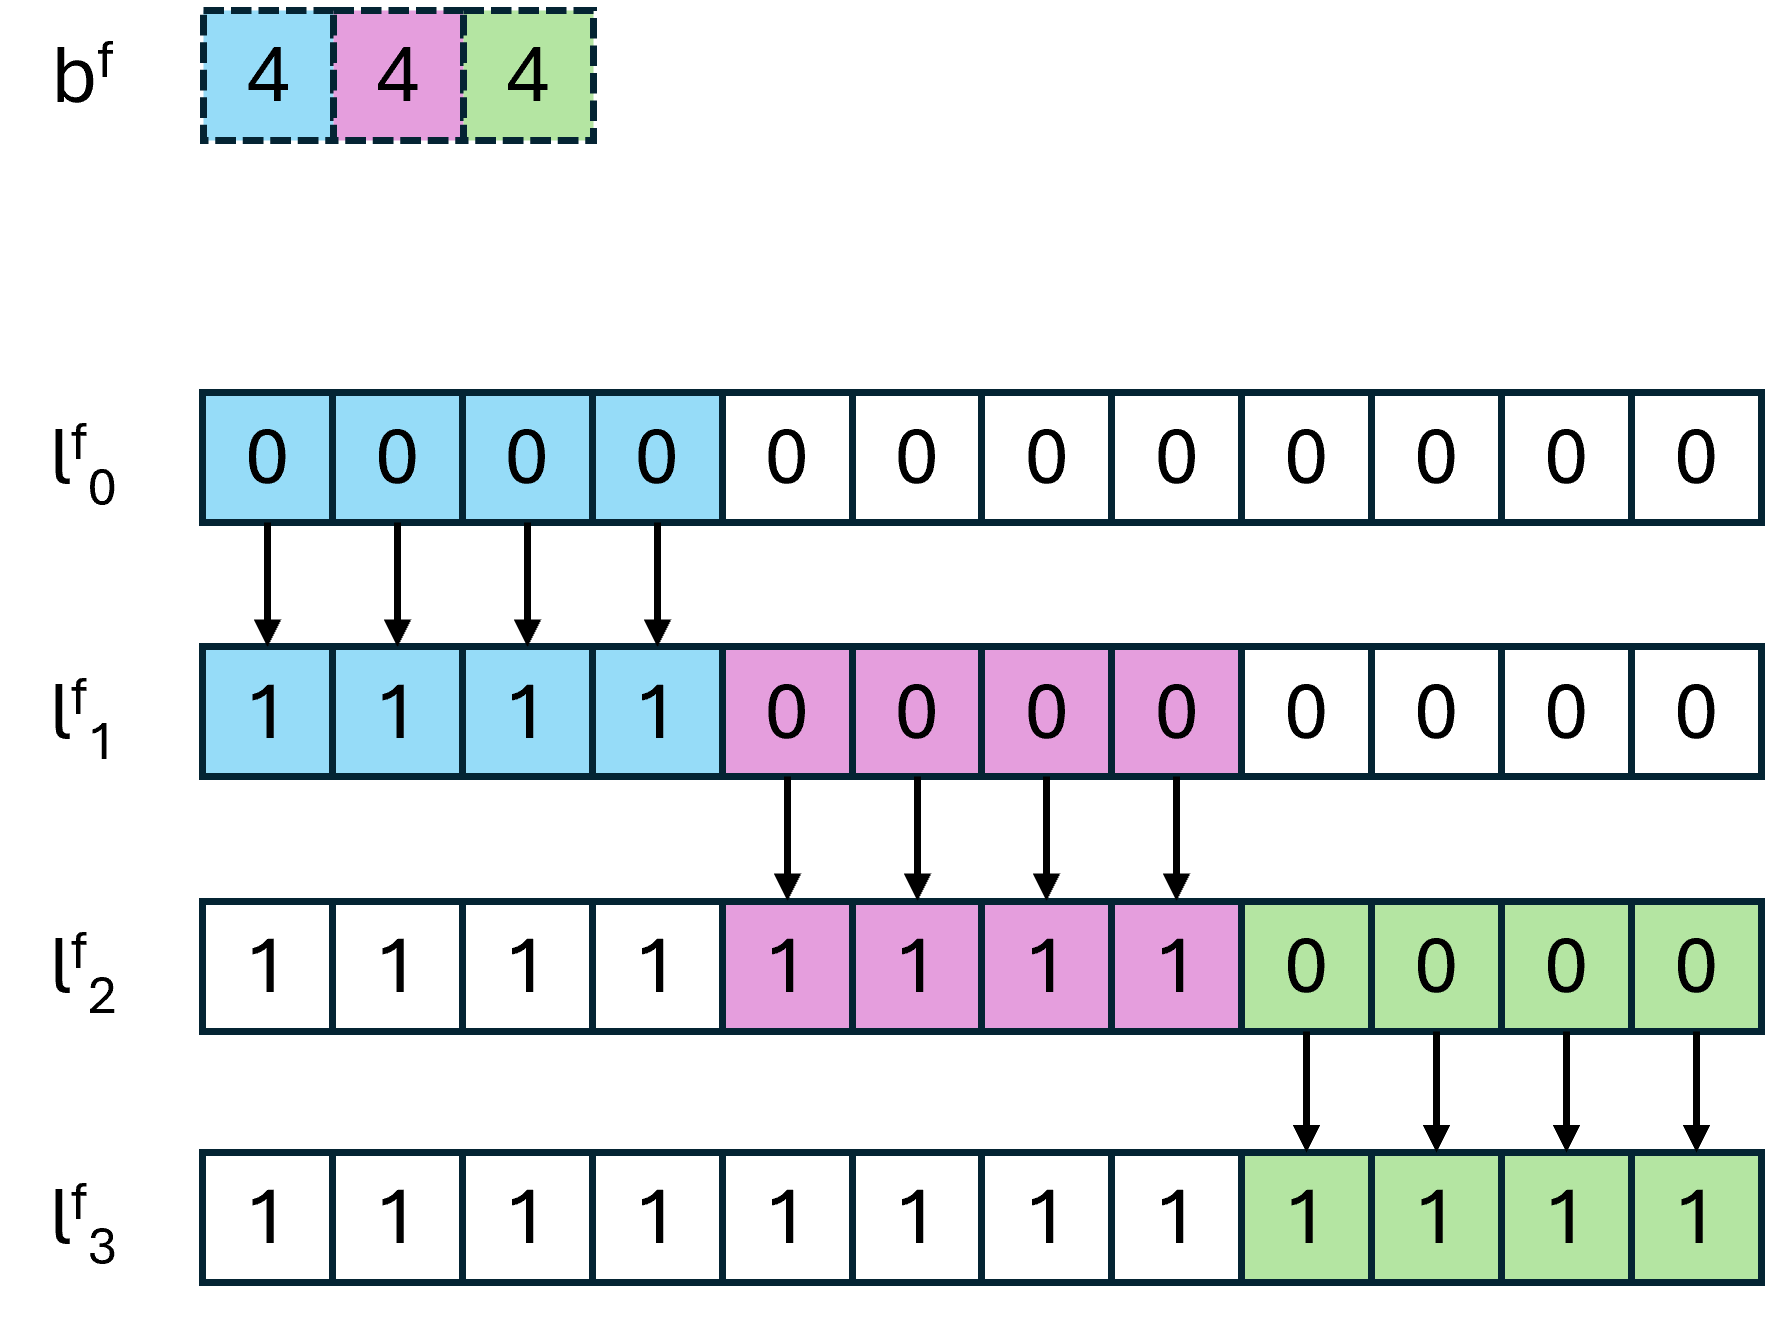
\includegraphics[width=\linewidth]{Images/bToCimNaive.png}

        \vspace{0.3em}
        \textbf{(a) Equally distributed bit-flip vector and corresponding CIM}
        \label{fig:cim_equal_spaced}
    \end{minipage}
    \hfill
    \begin{minipage}[t]{0.48\textwidth}
        \centering
        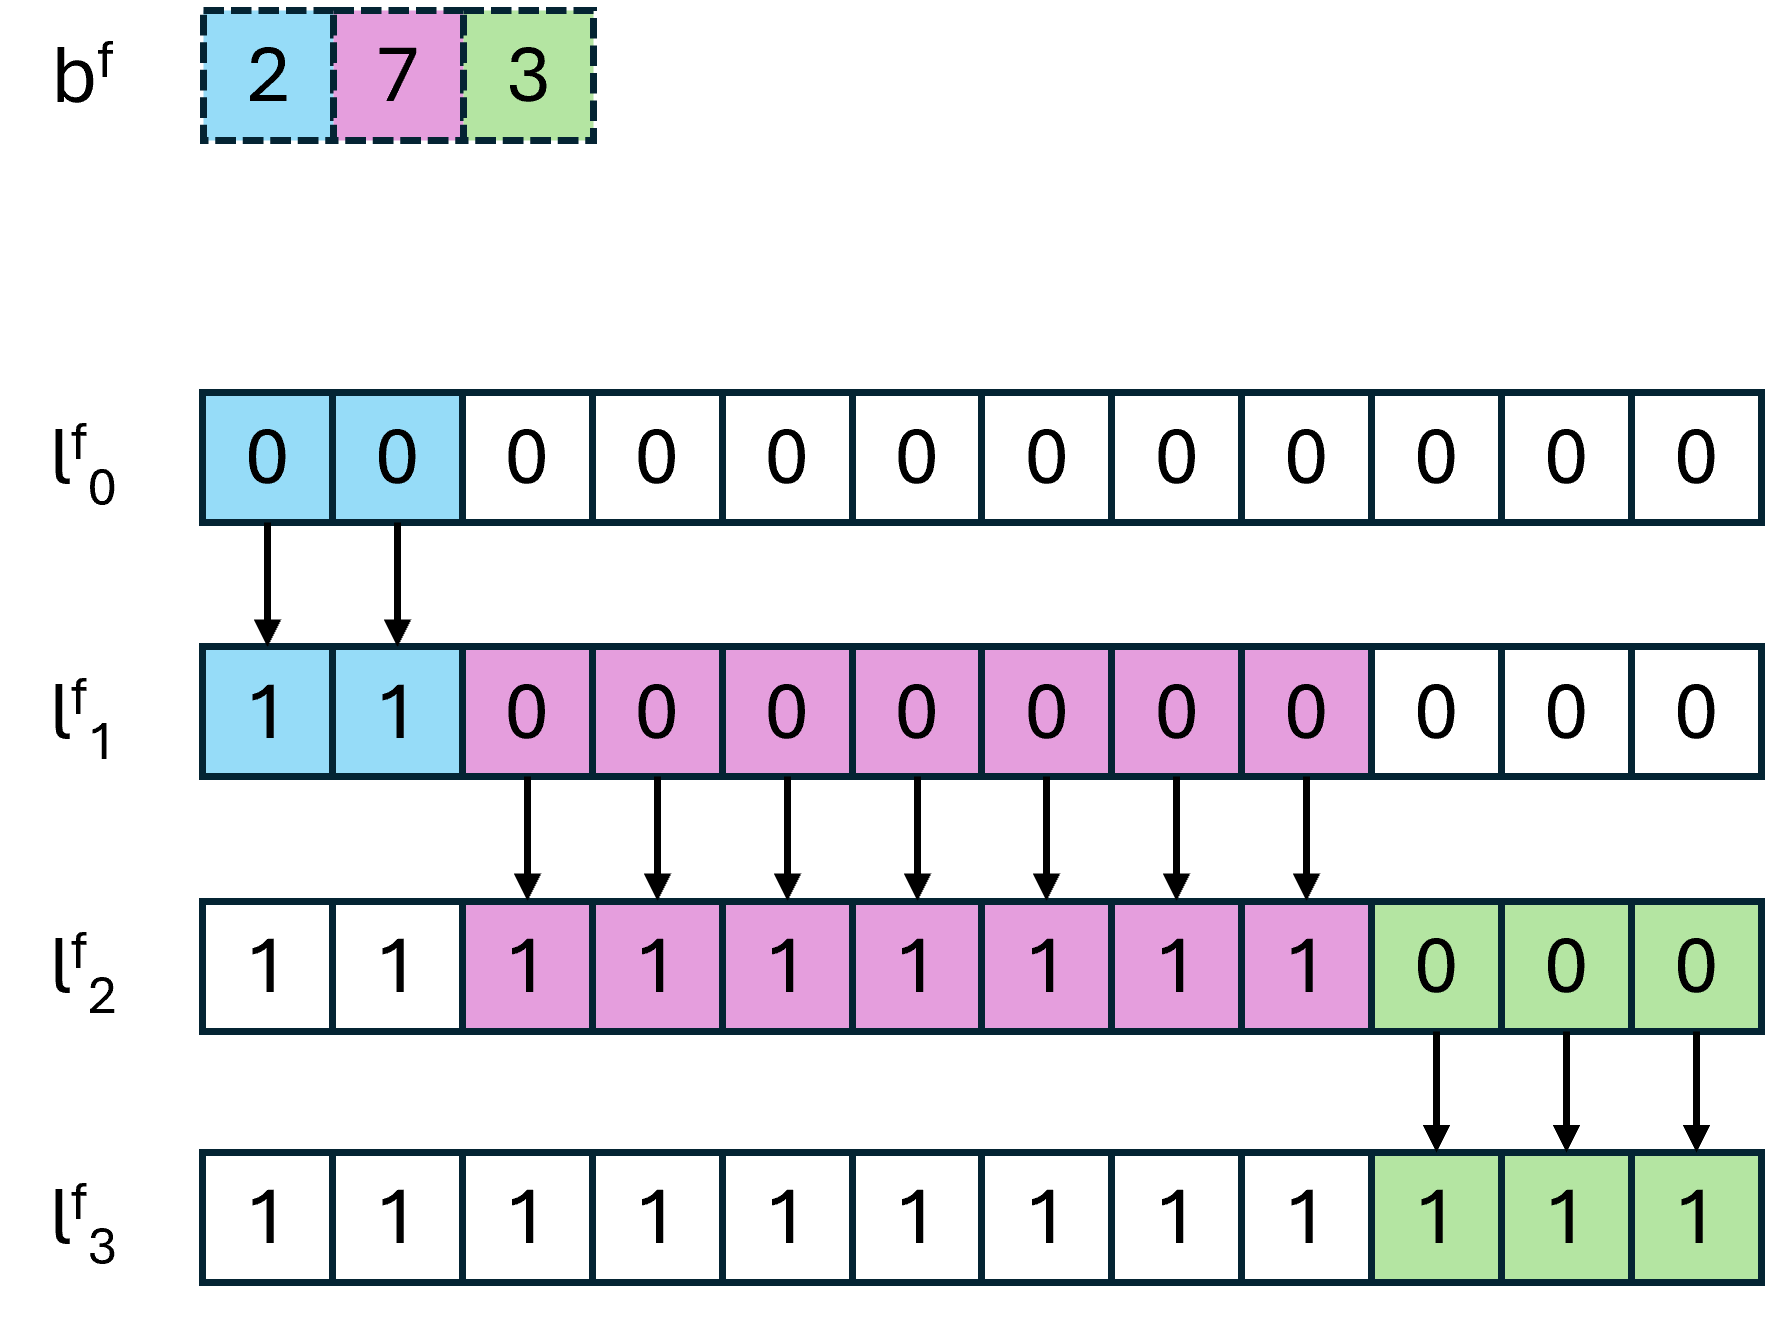
\includegraphics[width=\linewidth]{Images/bToCimOptimized.png}

        \vspace{0.3em}
        \textbf{(b) Non-equally distributed bit-flip vector and corresponding CIM}
        \label{fig:cim_distributed}
    \end{minipage}

    \caption{Illustrative comparison of equally spaced and non-equally distributed CIM generation for one feature. In both examples, the vector dimension is $D=12$ and the number of level transitions is three.}
    \label{fig:cim_generation_comparison}
\end{figure}

In the equally spaced example, every pair of consecutive level hypervectors has a Hamming distance of four. For the non-equally spaced example on the right with $\mathbf{b}^f=[2,7,3]$, the distance between level hypervectors $\boldsymbol{\ell}^f_{1}$ and $\boldsymbol{\ell}^f_{2}$ is increased to seven, while fewer bit flips are assigned to the other transitions. If distinguishing values mapped to levels 1 and 2 is particularly relevant for classification, this larger distance provides stronger separation between their representations in the hyperdimensional space $\mathcal{H}$. The central idea is therefore to redistribute the available bit-flip budget across the level transitions according to their relevance for the classification task, with the aim of increasing class vector separation and improving classification accuracy and robustness.\\

Which transitions should receive larger or smaller distances depends on the feature and the underlying EMG data and cannot be determined directly. Therefore, the complete bit-flip matrix $\mathbf{B}$ is optimized using a \ac{GA}. The optimization procedure is summarized in Algorithm \ref{alg:ga_cim_optimization}.

Initially, a population of $P$ bit-flip matrices $\mathbf{B}$ is generated. Although the equally spaced baseline matrix would provide an obvious starting point, initializing the complete population around this representation would reduce the diversity of the initial search space and could lead to premature convergence. Instead, a diverse initial population is generated by randomly distributing the fixed flip budget $D$ over the $L-1$ level transitions independently for every feature. For each row $\mathbf{b}^f$, random weights are drawn for all transitions, normalized to the total flip budget $D$, and rounded to integer values. A final correction ensures compliance with the sum constraint. For all GA experiments in this work, the population size is set to $P=128$, the number of generations to $G=64$, and the tournament size to $T=3$.

For every matrix $\mathbf{B}$ in the initial population, the corresponding \ac{CCIM} is generated and used to train an HDC model on the training data. The resulting model is then evaluated on the validation set. Validation accuracy forms the first optimization objective, while the similarity between the resulting class vectors forms the second objective and is minimized as a measure of class separation. Based on these two objectives, Pareto ranks and crowding distances are computed for the population.

The crowding distance measures how isolated an individual is from neighboring solutions within the same Pareto front. It is calculated independently for validation accuracy and class-vector similarity. Larger crowding distances generally indicate less densely populated regions of the Pareto front. In this way, the crowding distance can be used to preserve diversity among solutions with the same Pareto rank.


Starting from this initial population, the \ac{GA} is executed iteratively for $G$ generations. In each generation, $P$ new individuals are generated as an offspring population. For every offspring individual, two parents are selected from the current parent generation using tournament selection. In each tournament, $T$ individuals are sampled independently from the population and ranked. Candidates with a lower Pareto rank are preferred, and if two candidates have the same Pareto rank, the candidate with the larger crowding distance is selected. Since the tournament considers only $T$ randomly sampled individuals from the population, individuals that are not among the globally highest-ranked solutions can still be selected as parents. This preserves diversity in the population while introducing selection pressure toward better solutions.

The selected $P$ parent pairs are used to create $P$ offspring individuals through crossover and mutation. The two operators are described in detail in Sections \ref{sec:crossover} and \ref{sec:mutation}. Each resulting matrix  $\mathbf{B}$ is again converted into a \ac{CCIM}, used to train the HDC model, and evaluated in terms of validation accuracy and class-vector similarity.

Based on this evaluation, the parent and offspring populations are combined. The resulting $2P$ individuals are ranked using Pareto fronts, with validation accuracy as a maximization objective and class-vector similarity as a minimization objective. Complete Pareto fronts are selected successively until adding the next complete front would exceed the population size $P$. The remaining positions are filled with individuals from this front in descending order of crowding distance. By including the previous parent population in this selection, high-ranking individuals can survive across generations if they are not replaced by better candidates. This introduces an elitist component into the optimization to preserve good solutions from early generations while still allowing new solutions to enter the population.

After $G$ generations, the final matrix $\mathbf{B}^{\ast}$ is selected from the first Pareto front of the final population.  The individual with the highest validation accuracy is selected, with lower class-vector similarity used to resolve an exact accuracy tie. This matrix defines the optimized bit-flip distribution used to construct the final CCIM. The effect of this optimization on the HDC model is evaluated in Section \ref{sec:GA_results}.

\begin{algorithm2e}[htbp]
\caption{Genetic optimization of the CCIM representation}
\label{alg:ga_cim_optimization}

\KwIn{
    Population size $P$,
    number of generations $G$,
    tournament size $T$
}
\KwOut{
    Optimized bit-flip matrix $\mathbf{B}^{\ast}$
}

Initialize a population of $P$ random bit-flip matrices\;

\ForEach{individual in the population}{
    Generate CCIM from its bit-flip matrix\;
    Train HDC model\;
    Evaluate validation accuracy and class-vector similarity\;
}
Compute Pareto ranks and crowding distances\;
\For{$g \gets 1$ \KwTo $G$}{

    Initialize empty offspring population\;

    \While{offspring population contains fewer than $P$ individuals}{
        Select two parents independently using tournament selection with size $T$\;

        Generate child using ELC with crossover rate $70\%$\;
        Mutate child with mutation rate $20\%$\;

        Generate CCIM from the child\;
        Train HDC model\;
        Evaluate validation accuracy and class-vector similarity\;

        Add child to offspring population\;
    }

    Combine parent and offspring populations\;

    Compute Pareto ranks and crowding distances\;

    Select the best $P$ individuals as the next population\;
}

Select $\mathbf{B}^{\ast}$ from the first Pareto front\;
\Return{$\mathbf{B}^{\ast}$}\;

\end{algorithm2e}


    \subsection{Event-List Crossover}
    \label{sec:crossover}

    Together with mutation and selection, crossover is one of the main genetic operations in a \ac{GA}. Its purpose is to generate new candidate solutions by recombining useful structures from two parent individuals \cite{sudholt_crossover_2012}. For the bit-flip matrices $\mathbf{B}$, this means combining distributions already found in the parent matrices, particularly regions with high or low bit-flip densities, into a new candidate solution.
    
    Classical crossover operators directly exchange parts of the parent solutions. For segment-based crossover, the genome, in this case the matrix $\mathbf{B}$, is divided at several crossover points, and each segment of the child is inherited from one of the two parents \cite{spears_virtues_1995}. This allows parts of a parent solution to be preserved directly in the offspring. As an alternative, arithmetic crossover can be applied to numerical representations by combining corresponding values of both parents, for example through averaging or interpolation \cite{herrera_taxonomy_2003}.

    Arithmetic crossover is less suitable for the bit-flip matrices $\mathbf{B}$. Arithmetic recombination tends towards central values, and this averaging effect can reduce diversity in the population and produce smooth solutions \cite{herrera_taxonomy_2003}. However, this is not the intention when optimizing $\mathbf{B}$. Instead, the goal is to allow bit flips to accumulate at specific level transitions rather than distributing them equally. Consequently, useful patterns that have already emerged in the parent solutions could be smoothed out and partially lost through arithmetic crossover. Segment-based crossover could preserve such clusters of bit flips while still recombining information from two parents, but it introduces another important problem. For every feature, the total number of bits flipped between the first and last level hypervector must remain exactly $D$ in order to satisfy the sum constraint. However, this is not guaranteed, since the child may inherit segments containing comparatively high or low bit-flip counts from both parents, resulting in a total number of bit flips different from $D$. Therefore, a different crossover operator is required in this case.

    
    The solution is a problem-specific \ac{ELC}. The idea is to perform segment-based crossover not directly on $\mathbf{b}^f$, where it could violate the sum constraint, but on an event-list representation $\mathbf{e}^f$ of $\mathbf{b}^f$ instead. The first step is to transform $\mathbf{b}^f$ into an event list $\mathbf{e}^f$ of length $D$. Each element of this list corresponds to one bit flip, while its value denotes the level transition to which this bit flip is assigned, corresponding to an index in $\mathbf{b}^f$. The central idea is that, while $\mathbf{b}^f$ stores the number of bit flips per level transition, $\mathbf{e}^f$ stores every individual bit-flip event. Recombining two event lists therefore cannot change the total number of bit flips, but only their distribution across the level transitions. The transformation is performed by reading $b^f_i$ for every transition $i$ and inserting the transition index $i$ exactly $b^f_i$ times into the event list. 

    After transforming both parent vectors $\mathbf{b}^f_A$ and $\mathbf{b}^f_B$ into the event lists $\mathbf{e}^f_A$ and $\mathbf{e}^f_B$, segment-based crossover can be applied to them. The equal-length parent event lists are divided into segments, and the child event list $\mathbf{e}^f_C$ is constructed by inheriting each segment from either parent $A$ or parent $B$. Afterwards, $\mathbf{e}^f_C$ is converted back into the bit-flip vector $\mathbf{b}^f_C$ by counting how often each transition index occurs in the event list. Since $\mathbf{e}^f_C$ has the same fixed length as both parent event lists, the sum constraint is satisfied by construction.
    
    


    Figure \ref{fig:event_list_crossover} illustrates the \ac{ELC} for two exemplary bit-flip vectors with five level transitions and a total bit-flip budget of $D = 12$. Both vectors are first transformed into event lists with 12 elements. The event lists are then divided into four segments of three events, which are recombined by selecting each segment from one of the two parents. The resulting child event list is finally transformed back into a bit-flip vector, forming the child generated by the crossover.
    
        \begin{figure}[htbp]
            \centering
            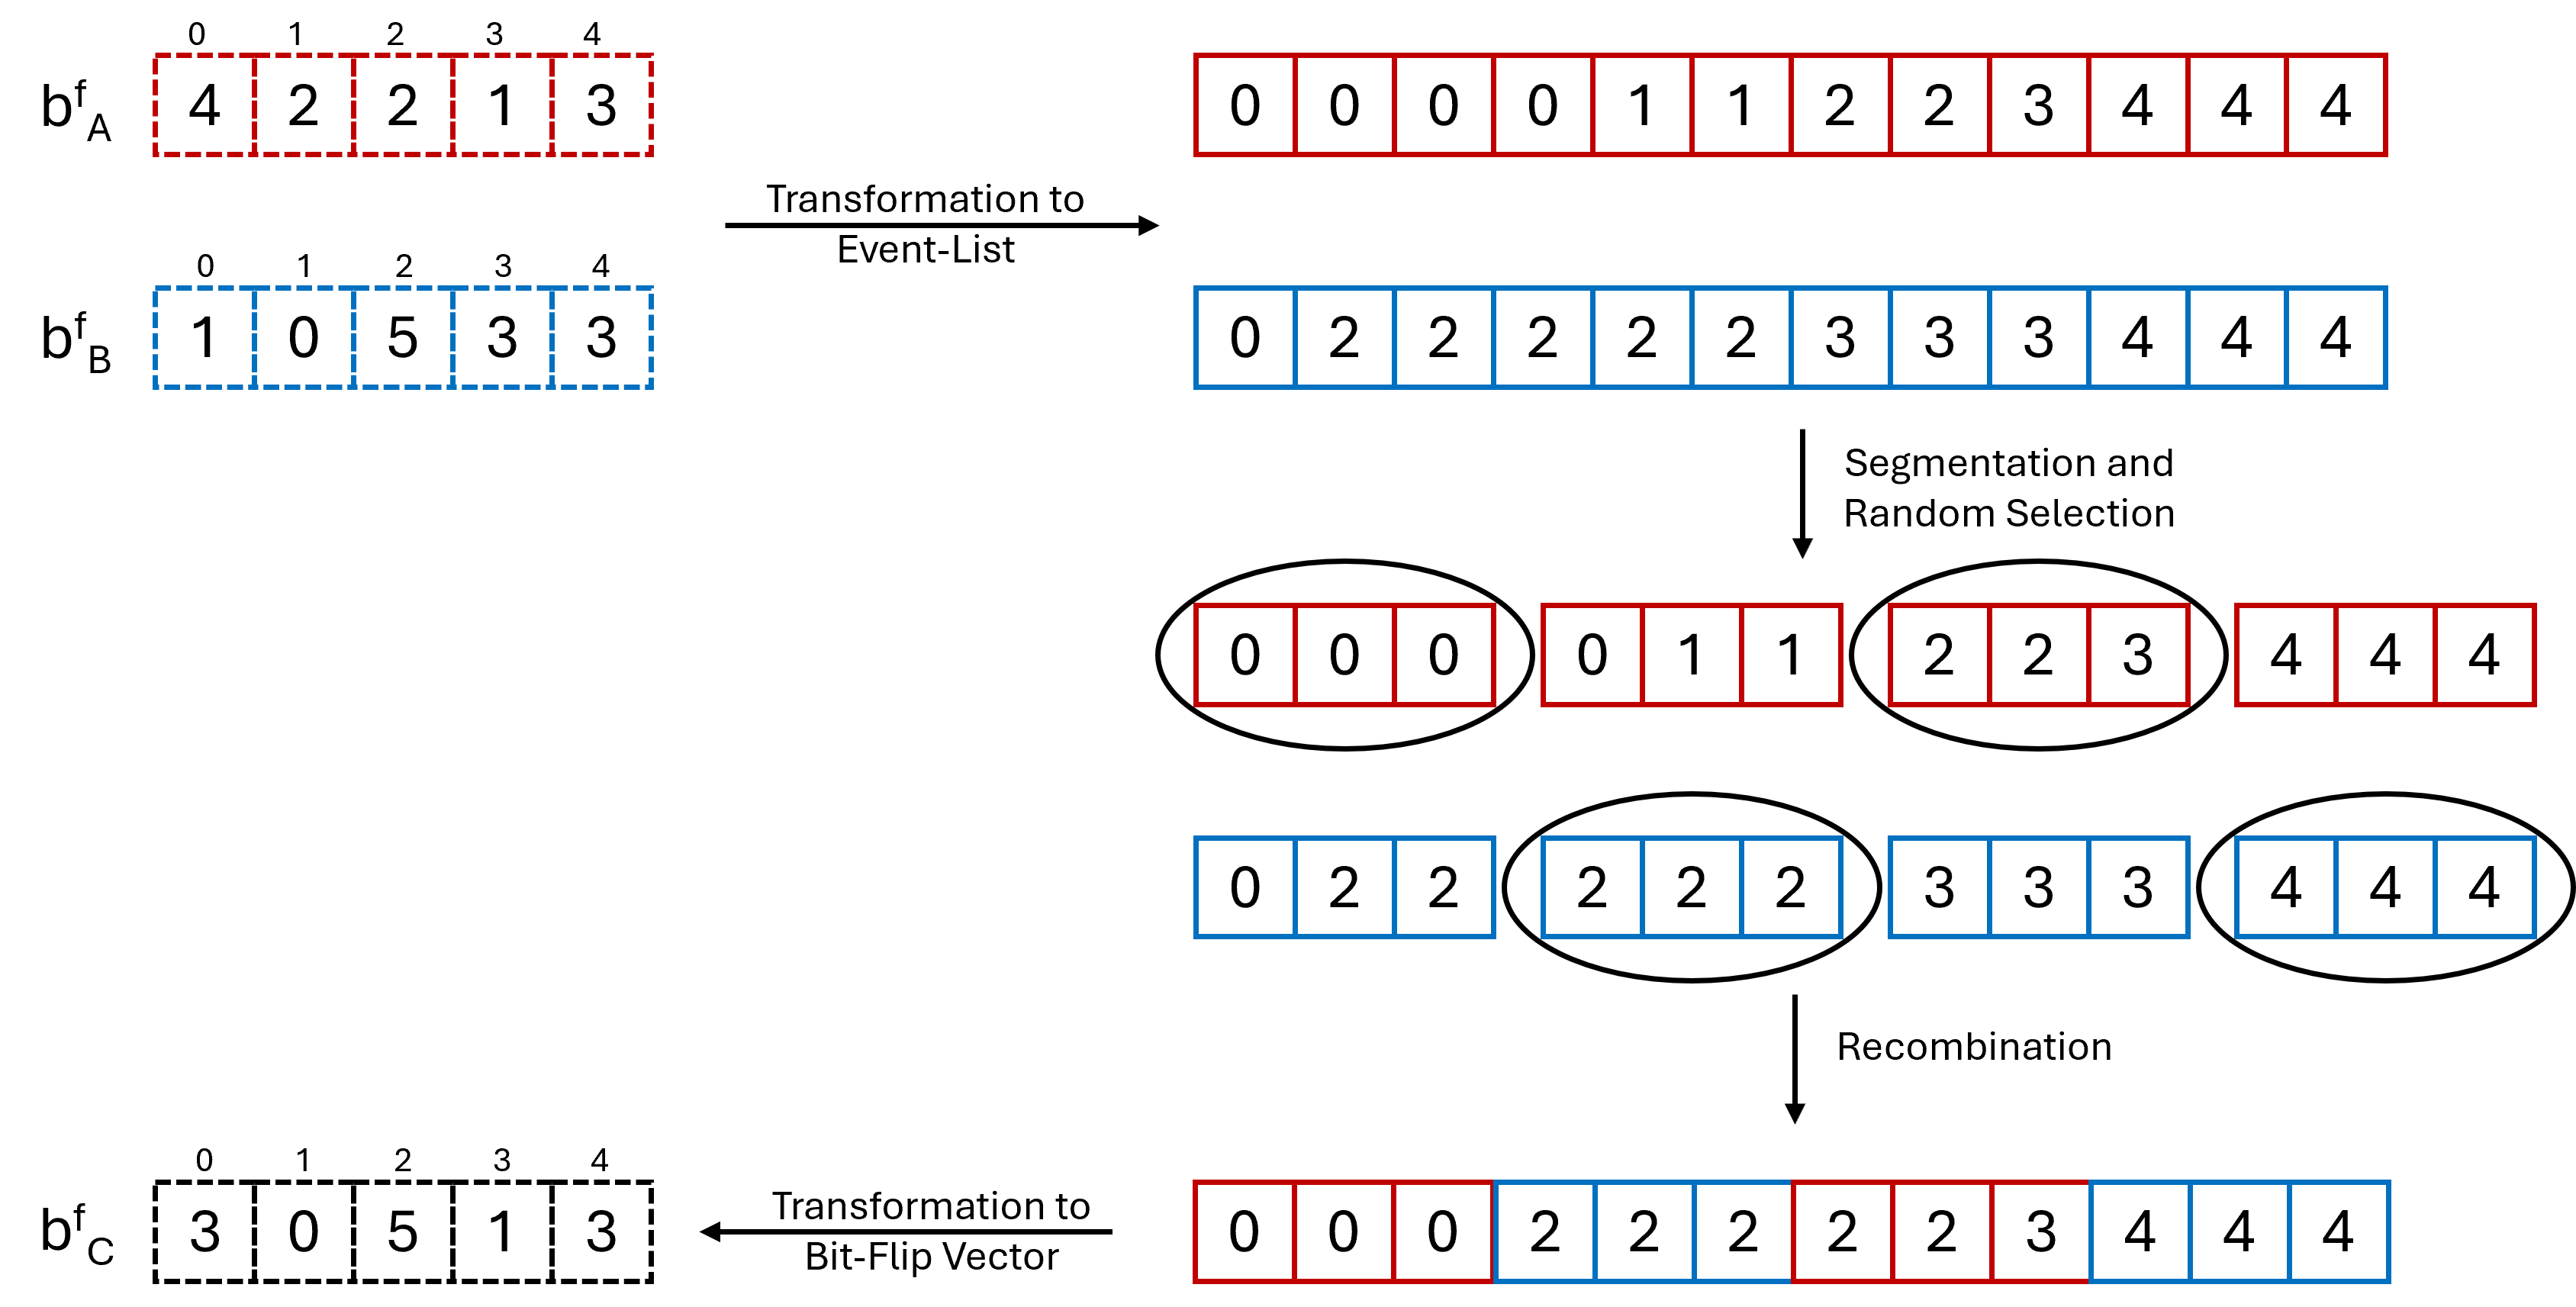
\includegraphics[width=\textwidth]{Images/ELC.png}
            \caption{Exemplary concept of the Event-List Crossover. The parent bit-flip vectors are first transformed into event lists. Crossover is then applied to segments of the event lists, and the resulting child event list is transformed back into a bit-flip vector.}
            \label{fig:event_list_crossover}
        \end{figure}
        
     A closer look at the example shows that parent $\mathbf{b}^f_A = [4, 2, 2, 1, 3]$ contains a peak of bit flips at index 0 and a minimum at index 3, while $\mathbf{b}^f_B = [1, 0, 5, 3, 3]$ has a peak at index 2 and a minimum at index 1. In the resulting child $\mathbf{b}^f_C = [3, 0, 5, 1, 3]$, the peak at index 2 inherited from $\mathbf{b}^f_B$, and the minima at indices 3 and 1 originating from $\mathbf{b}^f_A$ and $\mathbf{b}^f_B$, respectively, are preserved. Although the preservation of these structures during crossover is not guaranteed, it is more likely when complete segments rather than individual events are inherited. A peak in the bit-flip vector results in multiple consecutive occurrences of the same transition index in the event list. In this way, inheriting a segment that overlaps such a region can transfer several of these events together to the child.
     
    The degree to which characteristic extrema of both parents are preserved during crossover is therefore influenced by the segment size. Larger segments preserve longer parts of the parent event lists, while smaller segments allow more frequent switching between the two parents and therefore produce more new combinations. In GAs, this corresponds to the balance between exploration and exploitation. Early generations should provide sufficient exploration of different new candidate solutions, while later generations can increasingly exploit structures found in previous generations and refine them further. To realize this behavior in the ELC, the average segment size is adapted over the course of the optimization. The first generation uses an average segment size $\mu_{\min}$ of 0.5\% of $D$, while the final generation has an average segment size $\mu_{\max}$ of 15\% of $D$. For intermediate generations, the average segment size $\mu_g$ is interpolated geometrically as shown in Equation \ref{eq:chunk_size_mean}.
    
\begin{equation}
\mu_g =
\mu_{\min}
\left(
    \frac{\mu_{\max}}{\mu_{\min}}
\right)^{
    \frac{g-1}{G-1}
}.
\label{eq:chunk_size_mean}
\end{equation}

    Structures whose extent aligns well with a constant segment size could be more likely to be preserved than larger structures that are split across multiple segments, which may lead to segmentation artifacts. To reduce this effect, the specific size of every segment is sampled uniformly from an interval of $\pm20\%$ around the generation-dependent average segment size $\mu_g$, as shown in Equation \ref{eq:chunk_size_sampling_range}.
    
    \begin{equation}
        \mu \sim
        \mathcal{U}_{\mathbb{Z}}
        \left(
        \left\lfloor 0.8\mu_g \right\rfloor,
        \left\lfloor 1.2\mu_g \right\rfloor
        \right).
    \label{eq:chunk_size_sampling_range}
    \end{equation}
    
    Since both the segment sizes and consequently the segment boundaries in the event list are randomized, a remaining segmentation artifact could result from the first segment always starting at the first event of the list. To avoid this fixed alignment, a random offset is selected and the event list is cyclically shifted by this offset before crossover. Consequently, the segment boundaries are aligned with different positions of the event list for different crossover operations.
    
    The complete procedure is applied independently to every feature with a crossover rate of 70\%. This means that for 30\% of the features, the complete bit-flip vector $\mathbf{b}^f_A$ of parent A is copied to the child, while for the remaining 70\%, the \ac{ELC} is applied as described above.

    
    \subsection{Mutation}
    \label{sec:mutation}
    The mutation operator aims to introduce small perturbations into existing solutions to explore variations that cannot be generated by crossover alone. Without mutation, the GA could only recombine solutions already contained in the current population, but could not introduce new variations independently of the existing solutions. Mutation therefore contributes both to the local refinement of solutions and to maintaining diversity in order to reduce the risk of premature convergence \cite{hassanat_enhancing_2016}.
    
    Since directly adding or removing bit flips would violate the sum constraint, the event-list representation is also used for mutation. To preserve the total number of bit flips, a transport-based mutation is applied. Instead of adding or removing events, existing events are moved to neighboring level transitions. More specifically, mutating an event means changing its transition index in the event list by either $+1$ or $-1$. Since the number of events in the list remains unchanged, the total number of bit flips and therefore the sum constraint are preserved.

    Mutation is applied independently to every event of every feature with a probability of 20\%. If an event is selected for mutation, a direction is chosen randomly and its transition index is either increased or decreased by one. At the boundaries, cyclic wrapping is applied such that decrementing an event at the first transition maps it to the last transition and vice versa. This prevents the boundary transitions from having only one possible mutation direction, thereby reducing potential boundary artifacts.
    
    After mutation, the modified event list $\mathbf{e}^f$ is converted back into the corresponding bit-flip vector $\mathbf{b}^f$, and the resulting vectors of all features form the mutated matrix $\mathbf{B}$.



\section{Quantization}
\label{sec:quantization}
While the previous section described the optimization of where level hypervectors lie in hyperdimensional space $\mathcal{H}$ to improve class separability, the second major optimization in this work concerns how EMG values are mapped to these levels through quantization. As discussed in Section \ref{sec:optimizationOfHDCRelatedWork}, Ledwig \cite{ledwig_vdl-implementierung_2025} showed through the evaluation of different level counts that the positions of the level boundaries in the input space have a strong influence on the resulting representation and classification accuracy. 

The main goal of optimizing quantization is therefore to increase classification accuracy for a fixed number of levels or, if possible, reduce the number of levels while maintaining the accuracy of the baseline model. This directly reduces the memory required by the \ac{CCIM}, since it contains $F\times L$ hypervectors and its size therefore scales linearly with the number of levels $L$.
    \subsection{Methods}
    Quantization describes the process of mapping continuous EMG values from the input space to one of $L$ discrete levels indexed from $0$ to $L-1$. In the following, the partitioning of the input space into these discrete intervals is also referred to as binning. For every feature $f$, a set of $L-1$ thresholds $\boldsymbol{\tau}^f =[\tau^f_0,\tau^f_1,\ldots,\tau^f_{L-2}]$ is precomputed before HDC training. During encoding, the corresponding level can then be determined by comparing the feature value with the precomputed thresholds. If a value is exactly equal to a threshold, the lower adjacent level is selected. For the data-adaptive methods, the threshold vectors $\boldsymbol{\tau}^f$ are feature-specific, since the value distributions can differ between EMG electrodes and a suitable quantization for one feature is therefore not necessarily suitable for another. 

    The quantization methods evaluated in this work are grouped according to the information used to determine the thresholds. Apart from uniform binning, which is used by the baseline HDC model, two unsupervised methods, quantile binning and K-means binning, are implemented, as well as two supervised methods, decision-tree binning and ChiMerge binning.

    
        \subsubsection{Uniform Binning}
        \label{sec:UniformBinning}
        Uniform binning is the standard baseline and is used by the HDC model by default. It distributes the $L$ quantization levels uniformly over the value range, which is $[-1,1]$ for the EMG datasets used in this work, without considering the distribution of the data. The $L-1$ thresholds are placed between consecutive levels. In the implementation, Equation \ref{eq:uniform_binning_boundary} is used to precompute these thresholds with deterministic rounding and a resolution of $10^{-4}$, matching the quantization behavior of the original HDC model described in Section \ref{sec:background} and adopted from Ledwig's implementation \cite{ledwig_vdl-implementierung_2025}.

    The computation is performed using fixed-point integer arithmetic with a resolution of \(10^{-4}\). Thus, the real-valued range \([-1,1]\) is internally represented as the integer range \([-10000,10000]\). For threshold $i$, the term \(20000(i+1)-10000\), divided by $L-1$, determines the offset of the midpoint between the two corresponding uniformly spaced levels in the scaled representation. The ceiling operation followed by the subtraction of one implements the deterministic rounding behavior adopted from Ledwig’s quantization implementation \cite{ledwig_vdl-implementierung_2025}. Finally, subtracting \(10000\) shifts the result to the signed integer range corresponding to \([-1,1]\), and division by \(10000\) converts the scaled integer value back to a floating-point threshold.
    
        \begin{equation}
            \tau_i =
            \frac{
                \left\lceil
                    \frac{20000(i+1)-10000}{L-1}
                \right\rceil
                -1-10000
            }{10000},
            \qquad i=0,\ldots,L-2.
        \label{eq:uniform_binning_boundary}
        \end{equation}

        Uniform binning is the only evaluated method that is feature-independent, since its thresholds are determined only by the predefined value range and $L$, without using the training data. It therefore cannot adapt its boundaries to differences in the value distributions of individual features. It is also the most hardware-friendly of the evaluated methods, although this advantage is secondary in the proposed system because the thresholds are computed only once before training.

        
        \subsubsection{Quantile Binning}
        \label{sec:quantileBinning}

            Quantile binning is the first unsupervised method that uses the distribution of the training data and is therefore data-dependent. The main idea is to set thresholds such that the training samples are distributed approximately equally across the $L$ levels. While with uniform binning some levels may be rarely used or even unused because the corresponding value ranges contain few or no training samples, quantile binning aims to assign approximately the same number of EMG samples to every level. This results in a more balanced utilization of the available quantization levels and has the potential to improve the resulting HDC representation. Since the data distribution varies across features, separate thresholds are determined for each feature. 

            To compute the thresholds for one feature, all values of this feature in the training set are collected and sorted. The $L-1$ thresholds are then placed at the empirical quantiles according to Equation \ref{eq:quantile_binning_boundary}. $\mathbf{X}^f_{\mathrm{train}}=[x^f_0,x^f_1,\ldots,x^f_{n_{\mathrm{train}}-1}]$ denotes the sorted training values of feature $f$, with $n_{\mathrm{train}}$ as the number of training samples, and the function $\operatorname{interp}$ performs linear interpolation between neighboring sorted samples. If the quantile position lies exactly on a sample index, the corresponding sample value is used directly. Otherwise, the threshold is interpolated between the two adjacent samples.

                \begin{equation}
                \begin{aligned}
                \tau^f_{k-1}
                &=
                \operatorname{interp}
                \left(
                \mathbf{X}^f_{\mathrm{train}},
                \frac{k}{L}
                \right),
                \qquad
                k=1,\ldots,L-1,
                \\[0.5em]
                \operatorname{interp}
                \left(
                \mathbf{X}^f_{\mathrm{train}},
                q
                \right)
                &=
                (1-\alpha)x^f_{j_0} + \alpha x^f_{j_1},
                \\[0.5em]
                p
                &=
                q(n_{\mathrm{train}}-1),
                \qquad
                j_0=\lfloor p \rfloor,
                \qquad
                j_1=\lceil p \rceil,
                \\
                \alpha
                &=
                p-j_0.
                \end{aligned}
                \label{eq:quantile_binning_boundary}
                \end{equation}
           If repeated training values lead to two neighboring thresholds being equal or non-increasing, the later threshold is shifted to the next representable floating-point value. This preserves the required boundary order while changing the threshold only minimally. 
           
           Compared to uniform binning, quantile binning allocates more levels to dense regions of the feature distribution and fewer levels to sparse regions. 
           
        \subsubsection{K-Means Binning}
        \label{sec:K-meansBinning}

        K-means binning represents another data-dependent but unsupervised approach. While quantile binning distributes samples equally across bins, K-means binning instead uses the K-means clustering algorithm to search for representative centers of the EMG value distribution. The resulting thresholds are placed between neighboring cluster centers. 

        The clustering is performed separately for each feature and starts again by collecting and sorting all training values. Then $L$ cluster centers are initialized at interpolated quantile positions in the sorted training values. The algorithm repeatedly alternates between assigning each training value to its nearest center and updating each center to the mean of its assigned values. This is repeated until the center positions no longer change significantly or until the maximum number of iterations is reached. After convergence, the centers are sorted, and each threshold is computed as the midpoint between two neighboring centers. Since each value is assigned to its nearest center, these midpoints form the boundaries between neighboring clusters.

        K-means binning adapts the cluster centers to the shape of the feature distribution and can therefore represent regions with high concentrations of values more precisely. However, since the method does not use class labels, the resulting thresholds are still not necessarily aligned with class boundaries. This limitation is addressed by the following two supervised quantization methods.
        
        \subsubsection{Decision-Tree Binning}
        \label{sec:DecisiontreeBinning}
        
        Decision-tree binning is the first supervised quantization method evaluated in this work. In contrast to uniform, quantile, and K-means binning, it uses the class labels during the construction of the thresholds. The idea behind decision-tree binning is not to use the decision tree itself as a classifier, but to extract its split points as quantization boundaries. In this way, the resulting thresholds are chosen based on class separability rather than only on the distribution of feature values.

        The implementation fits one tree independently for every feature. First, all training samples are sorted by the value of the considered feature and treated as one interval. The goal is to repeatedly split the interval until $L$ subintervals are generated or no valid split remains. Therefore, the algorithm searches all currently existing intervals for the split that gives the largest reduction in sample-count-weighted Gini impurity. For each candidate split, the Gini impurities of the resulting intervals are weighted by their respective numbers of samples and compared with the weighted impurity of the interval being split.
        
        Gini impurity makes the method explicitly class-dependent. Its calculation is shown in Equation \ref{eq:gini_impurity}, where $n_c$ is the number of samples of class $c$ in an interval $S$, $|S|$ is the total number of samples in the interval, and $C$ is the number of classes.       
        A Gini impurity of 0 means that all samples in an interval belong to the same class, while increasingly mixed class distributions result in higher values of $\operatorname{Gini}(S)$. Therefore, a split is considered useful if it separates the samples into two intervals with more homogeneous class distributions. This means that the resulting thresholds are not necessarily placed in dense regions of the input distribution, but rather at positions that improve class separation. This is the main difference from quantile and K-means binning.
        
            \begin{equation}
                \operatorname{Gini}(S)
                =
                1 -
                \sum_{c=0}^{C-1}
                \left(
                    \frac{n_c}{|S|}
                \right)^2 .
            \label{eq:gini_impurity}
            \end{equation}
            
        The interval containing the best split is divided at the selected split position, and the corresponding threshold is placed halfway between the largest feature value of the left interval and the smallest feature value of the right interval. The procedure is repeated until either $L$ intervals are reached or no valid split remains. A split is only valid if both resulting intervals contain at least $\texttt{TREE\_1D\_MIN\_SAMPLES\_LEAF}=10$ samples. In addition, a candidate split is ignored if the two neighboring feature values differ by less than $\texttt{TREE\_1D\_THRESHOLD\_EPS}=10^{-12}$. This prevents thresholds from being placed between duplicate or numerically almost identical values. After tree construction, the resulting split thresholds are used directly for quantization.
        Since not every feature necessarily contains enough discriminative structure to produce \(L-1\) valid tree splits, the implementation includes a fallback mechanism. If fewer than $L-1$ thresholds are generated, the remaining thresholds are filled with quantile-based thresholds. Finally, duplicate or non-increasing thresholds are adjusted minimally to ensure strict ordering.

        Decision-tree binning therefore represents a supervised top-down approach, since it starts with one interval containing all training samples and creates finer intervals through splitting. To also evaluate the opposite family of supervised discretization methods, the next section introduces ChiMerge binning as a bottom-up approach.

        \subsubsection{ChiMerge Binning}
        \label{sec:ChiBinning}
            ChiMerge binning is the second supervised quantization method evaluated in this work. In contrast to decision-tree binning, ChiMerge follows a bottom-up approach, as it starts with a large number of small intervals and repeatedly merges neighboring intervals whose class distributions are most similar. 

            From the sorted values of each feature, the algorithm initially creates one interval for each distinct feature value. Each interval stores its value range, the number of contained samples, and a class histogram over the $C$ classes. The main idea is to repeatedly merge the two most similar adjacent intervals until only $L$ intervals remain. The similarity of two neighboring intervals is determined from their class histograms using the chi-square score.

            
            For two neighboring intervals $S_L$ and $S_R$, $n_{L,c}$ and $n_{R,c}$ denote the numbers of samples of class \(c\) in the left and right intervals, respectively. To determine whether the class distributions of the two intervals differ, these observed counts are compared with the counts that would be expected if both intervals followed the same combined class distribution. For class $c$, these expected counts are calculated as $E_{L,c}=|S_L|(n_{L,c}+n_{R,c})/(|S_L|+|S_R|)$ and $E_{R,c}=|S_R|(n_{L,c}+n_{R,c})/(|S_L|+|S_R|)$.
            The chi-square score then measures the deviation between the observed and expected counts, as shown in Equation~\ref{eq:chimerge_score}. Classes that do not occur in either interval are omitted from the calculation, since their expected counts are zero.
            
            A low chi-square score therefore indicates that the two intervals have similar class distributions and can be merged with comparatively little loss of class-separating information.
        

                \begin{equation}
                \chi^2(S_L,S_R)
                =
                \sum_{\substack{c=0\\n_{L,c}+n_{R,c}>0}}^{C-1}
                \left(
                \frac{(n_{L,c}-E_{L,c})^2}{E_{L,c}}
                +
                \frac{(n_{R,c}-E_{R,c})^2}{E_{R,c}}
                \right).
                \label{eq:chimerge_score}
                \end{equation}
            While the number of intervals is larger than $L$, the algorithm computes the chi-square score for every neighboring interval pair. The pair with the lowest chi-square score is merged, and the scores are recomputed for the updated set of intervals. After $L$ intervals are obtained, the $L-1$ thresholds are placed halfway between the intervals.
            
            Compared to decision-tree binning, ChiMerge does not search for the single best split in a larger interval. Instead, it preserves boundaries only where neighboring regions show different class distributions while removing boundaries between similar regions. This makes ChiMerge the bottom-up counterpart to the top-down decision-tree approach.\\
            
            All quantization methods produce the same output format, a threshold vector $\boldsymbol{\tau}^f$ of length $L-1$ for every feature. Therefore, the encoder and the following HDC pipeline remain unchanged, independently of the selected binning method. The quantization methods only differ in how the threshold positions are determined. Uniform binning is data-independent, quantile and K-means binning are unsupervised and use only the training values, while decision-tree and ChiMerge binning are supervised and additionally use the training labels. Their impact on HDC classification accuracy and the potential reduction of \ac{CCIM} memory through lower level counts is evaluated in Section \ref{sec:quantization_results}.\\
            

\section{FPGA Accelerator}
\label{sec:fpga_accelerator}
The previous sections described optimizations of the HDC model at the algorithmic level. 
First, redundant computations in the temporal encoding were reduced by reusing spatially encoded hypervectors. 
Then, the representation of the \ac{CCIM} was optimized with a \ac{GA}, and different quantization methods were introduced to improve the mapping from EMG feature values to discrete HDC levels. These methods improve the \ac{HDC} model itself, but they do not yet describe how the resulting pipeline can be executed efficiently on embedded hardware.

This chapter therefore describes the SystemC accelerator developed for FPGA execution of the optimized HDC pipeline. As discussed in Section \ref{sec:FPGA_background}, the binary vector operations used by HDC expose a high degree of parallelism and are well suited for FPGA implementation. The accelerator exploits this property through pipelining and different degrees of parallelism within the individual processing stages.

The accelerator does not implement the complete EMG processing workflow and is limited to the computational HDC datapath described in Section~\ref{sec:accelerator_pipeline}. Preprocessing, quantizer fitting, CCIM optimization, quantization, dataset handling, and experiment evaluation remain software tasks. 
The hardware accelerator receives already quantized EMG samples and implements spatial encoding, temporal N-gram construction, class-vector accumulation during training, and Hamming-distance computation during inference. The final class decision based on the computed distances is performed outside the accelerator.


\subsection{Hypervector Representation}
% 64-bit words
% VECTOR_WORDS = VECTOR_DIMENSION / WORD_BITS
% Why this matters for FPGA: bitwise operations over words.
In the algorithmic description, a hypervector is treated as a binary vector of dimension $D$. For the hardware implementation, the accelerator groups the vector dimensions into fixed-width words instead of representing them as individually addressed bits. Ledwig \cite{ledwig_vdl-implementierung_2025} uses a similar segmented representation in his VHDL implementation to reduce the hardware resource requirements. The word-based organization makes it possible to choose how many words are processed in parallel in each cycle. Processing more words per cycle reduces the required number of cycles, while processing fewer words allows the corresponding datapath to be reused across multiple cycles and therefore reduces hardware resource usage.


In the HDC accelerator the word width is fixed to $W = 64$ bits. The implementation requires the vector dimension $D$ to be divisible by $W$. Thus, one hypervector consists of $n_{\mathrm{words}} = \frac{D}{W}$ words and is represented as an array of $n_{\mathrm{words}}$ elements of 64 bits each. This representation is used for the CCIM, the associative memory, spatial encoding, training accumulation, and distance computation. The temporal encoding stage is an exception and internally uses a packed $D$-bit representation, since its permutation operation during N-gram construction can move bits across word boundaries. This is described in more detail in Section \ref{sec:accerator_ngram_stage}.

The word-based representation is well suited to the binary HDC operations. Binding can be performed as a bitwise XOR between corresponding words. During bundling, the bit positions within a word can be accumulated independently, while Hamming distance computation starts with a bitwise XOR followed by a population count for each word. The resulting partial Hamming distances are then added to obtain the Hamming distance over the complete hypervector.
Consequently, the representation does not change the HDC algorithm but provides a hardware-oriented organization that allows the degree of word-level parallelism to be adapted to the available hardware resources.

\subsection{Accelerator Pipeline}
\label{sec:accelerator_pipeline}

The accelerator implements the HDC processing chain as a sequence of pipeline stages. Each stage performs one part of the algorithmic pipeline and passes its result to the following stage. This separation has two main purposes. First, it allows different samples to be processed concurrently in different stages of the pipeline, thereby increasing throughput. Second, it makes the dataflow between the individual HDC operations explicit and allows the HLS tool to schedule and synthesize the operations of different stages independently.

The accelerator consists of four main processing stages for spatial encoding, temporal encoding, class-vector accumulation, and Hamming-distance computation, together with two additional stages for command handling and response generation. Each stage is implemented as a separate \texttt{SC\_CTHREAD} in SystemC. Incoming samples first pass through the command handling, spatial and temporal encoding stages. Afterwards, the temporal encoding stage routes the data according to the command type. During training, valid N-grams are forwarded to the training stage and accumulated into a class vector, while during inference, the N-grams are forwarded to the distance stage and compared with all stored class vectors. The computed distances are then passed to the response stage. The following sections describe the functional role and implementation of each stage.


Figure \ref{fig:accelerator_concept} illustrates the accelerator architecture and its main dataflow. The software controller is shown in orange, communicating with the accelerator through the AXI4-Stream wrapper in blue. The individual accelerator stages are shown in green, and the \ac{CCIM} and associative memory in purple. The arrows indicate the dataflow between the processing stages, while the separate memory-access paths show how the spatial encoder accesses the CCIM and how the associative memory is written during training and read during inference. The details of the communication interfaces, memory organization, and the individual stages are described in the following sections.



\begin{figure}[htbp]
    \centering
    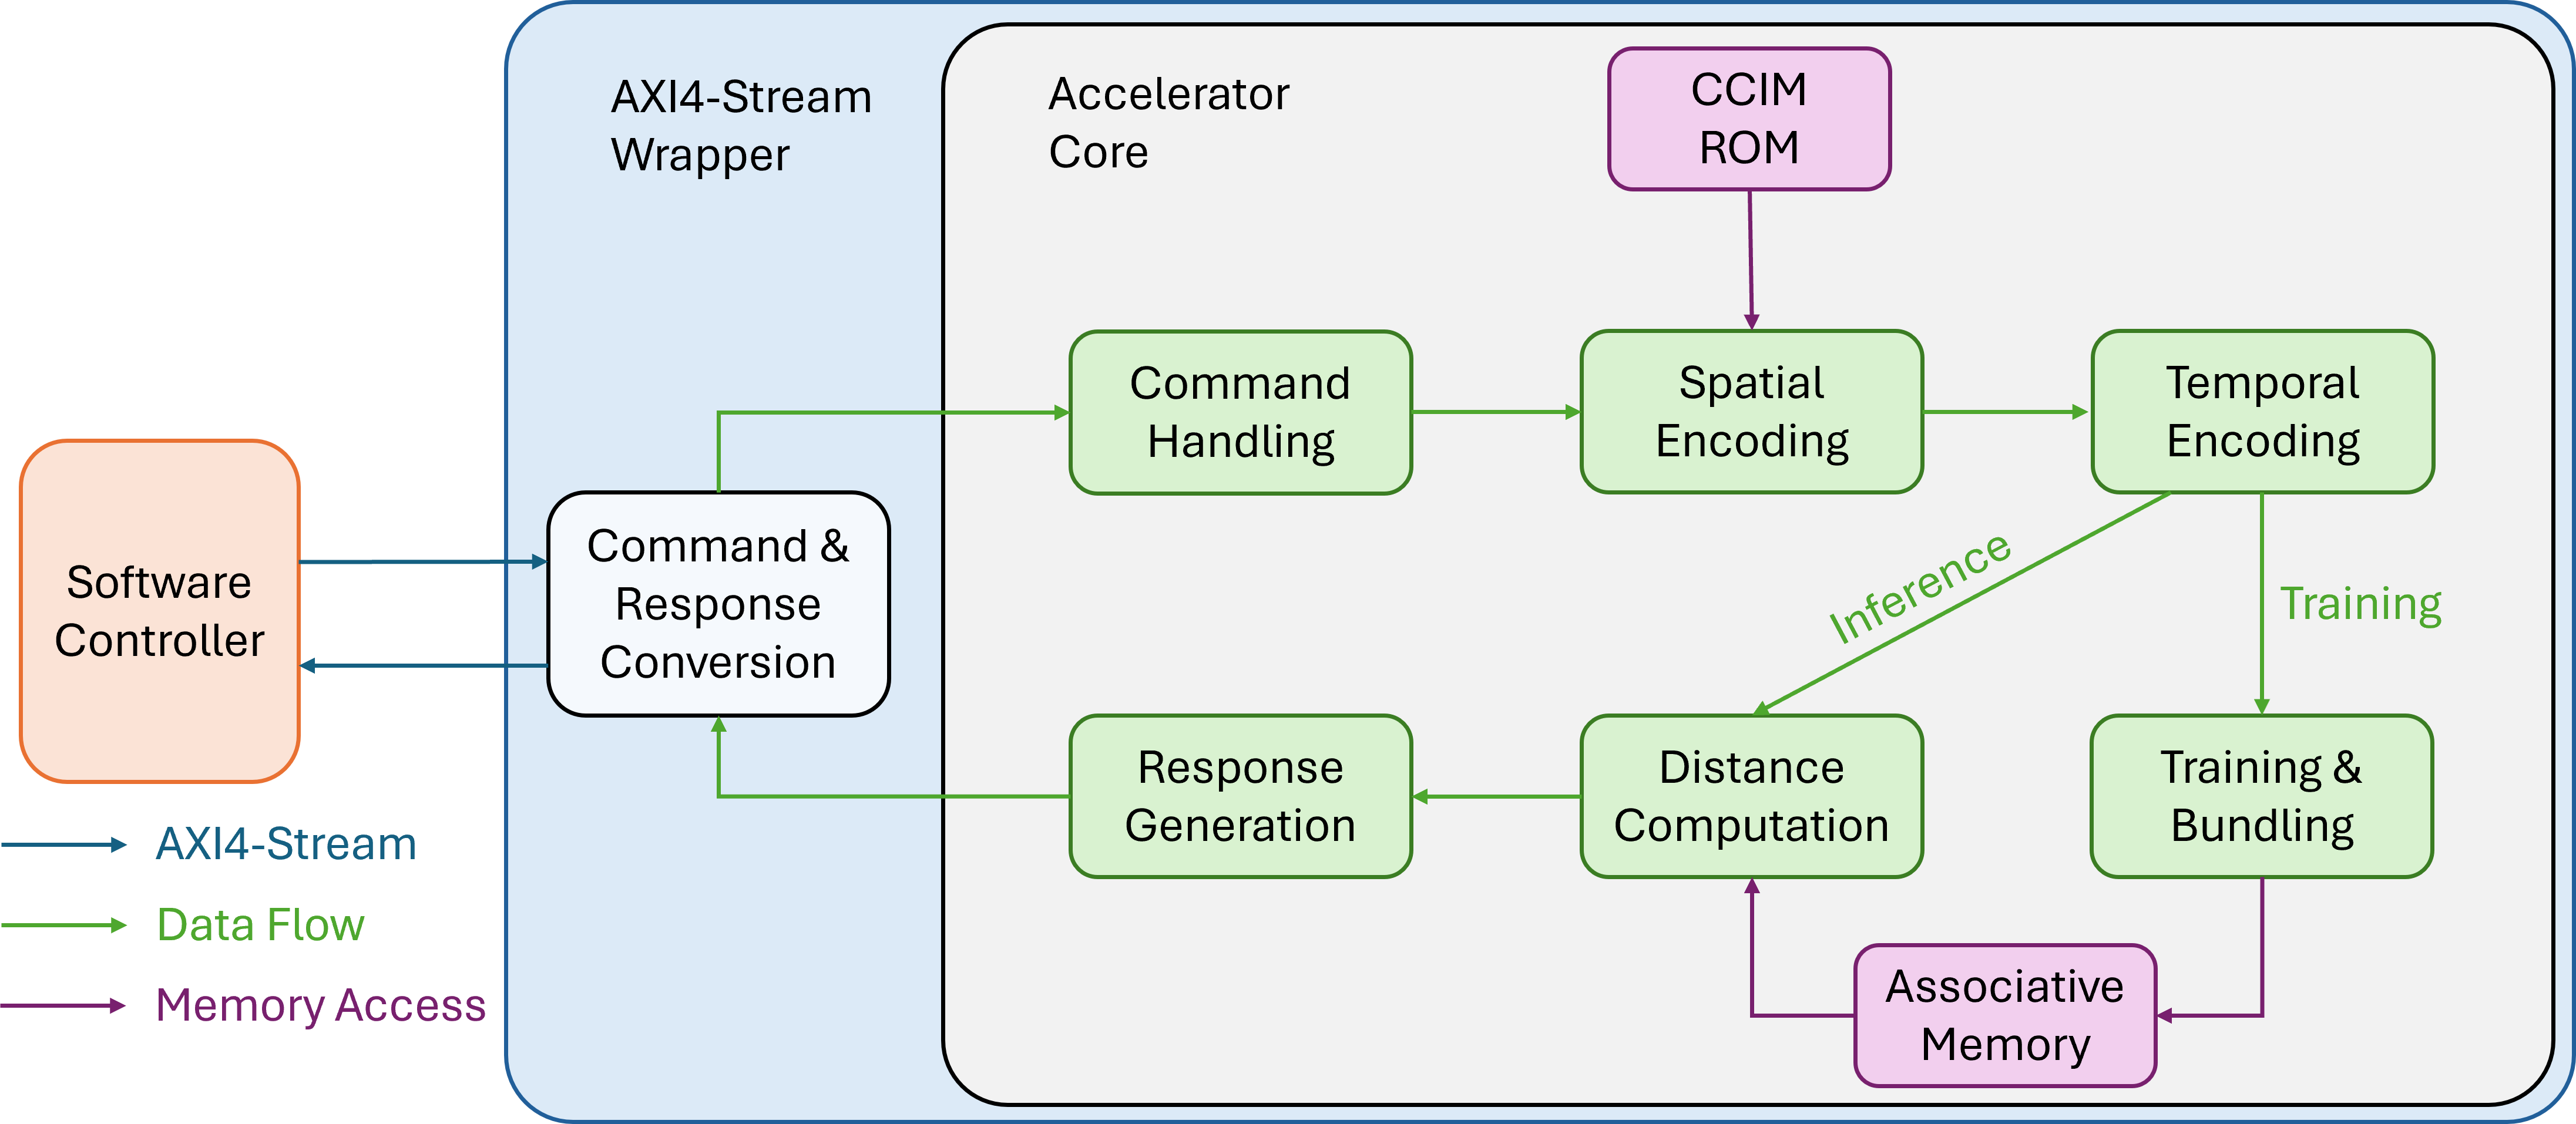
\includegraphics[width=\textwidth]
    {Images/accelerator.png}
    \caption{Overview of the HDC accelerator architecture and dataflow between the software controller in orange, AXI4-Stream wrapper in blue, accelerator pipeline in green, and internal model memories in purple.}
    \label{fig:accelerator_concept}
\end{figure}

    \subsubsection{Command Handling}
    %command stage
    The command stage forms the input stage of the accelerator core and receives commands from the software-side controller described in Section \ref{sec:controller}. It converts each command into an internal packet and forwards it to the spatial encoder. A command contains a command type, a sample consisting of 32 quantized EMG values, and, for training commands, the corresponding class ID. The command type determines how the packet is processed by the following pipeline stages. 
    
    The two types of data commands are \texttt{TrainSample} and \texttt{InferSample}. Both commands are forwarded directly into the pipeline, where the included sample is encoded. Training N-grams are then accumulated into a class vector, while inference samples are compared with the already trained \ac{AM}. The command stage does not wait for a data command to complete before accepting the next one, which allows consecutive samples to enter the accelerator while previous samples are still processed by later pipeline stages. 
    
    Control commands, in contrast, mark boundaries in the data stream and therefore require synchronization with the affected pipeline stages. They are propagated through the pipeline without encoding a sample, and the command stage waits for a completion signal before accepting further input. Three control commands are used. 

    \texttt{ResetTraining} clears both the temporal N-gram state and the current training accumulation state before a new training sequence. This prevents buffered hypervectors from the previous temporal context or unfinished bundling scores from influencing the next training sequence.

    \texttt{InvalidTrainingStep} marks a class boundary or the end of a training sequence. It clears the temporal context and, if valid N-grams have been accumulated, finalizes the current class vector by thresholding the bundling scores and writing the resulting hypervector to the associative memory.

    Finally, \texttt{ResetInference} clears only the temporal N-gram state before a new inference sequence. Since it does not modify the training state or associative memory, its completion only has to be confirmed by the temporal encoding stage.

    Through this distinction between non-blocking data commands and synchronized control commands, the command stage allows samples to flow continuously through the pipeline while ensuring that temporal and training state cannot propagate across sequence or class boundaries.
    
    \subsubsection{Spatial Encoding}
    
    The spatial encoding stage transforms one quantized EMG sample into one binary hypervector. For data commands, the incoming packet contains one quantized level index for each of the $F=32$ EMG features. These indices are used to retrieve the corresponding feature-specific level hypervectors from the \ac{CCIM}, which are then bundled into one spatial hypervector. Control commands do not contain samples to be encoded and are forwarded to the temporal encoding stage without further processing.

   The bundling operation is performed on the word-based representation described in the previous section. For each word position, the corresponding 64-bit word is retrieved from the selected CCIM hypervector of all 32 features. The implementation processes all features in parallel. For every bit position, a signed score is accumulated across the 32 feature hypervectors, with +1 for a one and -1 for a zero. The resulting output bit is set to one if the final score is greater than or equal to zero, implementing the majority operation described in Section \ref{sec:implementation_improvements}. All 64 bit positions within a word are processed in parallel.

    In addition to this feature- and bit-level parallelism, the number of hypervector words processed in one cycle can be varied. Processing more words in parallel reduces the number of cycles required for spatial encoding, but also requires additional CCIM read bandwidth and replicated bundling logic. Processing fewer words allows the same datapath to be reused over multiple cycles and reduces the corresponding hardware requirements. The memory organization that enables the required parallel CCIM accesses is described in Section~\ref{sec:accelerator_memory}.\\

    After all hypervector words have been processed, the resulting spatial hypervector is forwarded to the temporal encoding stage.
    
    \subsubsection{Temporal Encoding}
    \label{sec:accerator_ngram_stage}

    The temporal encoding stage receives the spatial hypervectors and combines consecutive samples into N-gram hypervectors. This corresponds to the temporal encoding described in Section \ref{sec:Encoding} and adds information about the recent sequence of EMG samples to the spatial representation.

    The stage stores the most recent spatial hypervectors in a ring buffer of size $N$. When a new data sample arrives, its encoded hypervector is written into the buffer and the write position is advanced. As long as fewer than $N$ valid spatial hypervectors are available, for example at the beginning of a sequence or after a control command that resets the temporal context, no valid N-gram can be generated. In this case, the stage forwards a packet with the validity flag set to false. 
    Once the buffer is filled, every newly arriving sample enables the generation of a new N-gram.

    In contrast to the word-based processing of the other stages, the temporal encoder internally represents each hypervector as one continuous $D$-bit value. This is particularly useful for permutation. While binding can be performed independently for every word, a one-bit cyclic permutation always moves bits across the boundaries between neighboring 64-bit words. A word-based implementation would therefore require explicit handling of these boundary bits for every permutation. With the continuous representation, the permutation can instead be applied directly to the complete hypervector by cyclically shifting all $D$ bits by one position. The subsequent binding operation is performed as a bitwise XOR over the complete $D$-bit vector.

    This implementation exploits full bit-level parallelism within each permutation and binding operation. Compared with processing the hypervector word by word, this avoids iterating over the $n_{\mathrm{words}}$ words for every permutation and binding operation and therefore reduces the number of cycles required for temporal encoding. The trade-off is a $D$-bit-wide permutation and XOR datapath, which requires more parallel logic and can increase routing complexity and timing pressure.\\

    Control commands reset the temporal context whenever samples from different sequences must not contribute to the same N-gram. At the beginning of inference, after a training reset, and at class transitions during training, the ring-buffer write position and the number of valid buffered hypervectors are reset. The previously stored spatial hypervectors are therefore no longer considered part of the current sequence. The following samples first refill the N-gram buffer and are forwarded as invalid N-grams until $N$ valid samples are available again.

    \subsubsection{Training and Bundling}

    The training stage receives the N-gram packets from the temporal encoding stage and constructs the class hypervectors during training. Only valid training N-grams are accumulated, while invalid N-grams are simply ignored.

    For every class, the training N-gram hypervectors are bundled by accumulating a signed score for each hypervector dimension. A bit value of one contributes +1 to the corresponding accumulator, while a zero contributes -1. Once all N-grams of a class have been processed, the accumulated scores are thresholded according to the bundling rule described in Section \ref{sec:implementation_improvements} to generate the final binary class vector, which is then stored in the \ac{AM}.

    The accumulation uses the previously described 64-bit word representation. Within each word, the 64 bit positions are updated independently and therefore in parallel.

    As in the encoder, the number of words processed in one cycle can be varied. Processing more words in parallel reduces the number of steps required to add an N-gram to the accumulator and to finalize a class vector, but requires more parallel logic and memory accesses. Processing fewer words reuses the same hardware across several word groups and consequently reduces the required resources.

    
    Class boundaries are indicated by the control commands described previously. When the current training sequence is finalized, the accumulated scores are converted into the corresponding class hypervector and written to the associative memory. The accumulation state is then cleared before samples of the next class are processed. This prevents training information from different classes from being combined.

    \subsubsection{Distance Computation}
    
    The distance computation stage is used during inference. It receives valid query hypervectors from the temporal encoding stage and compares them with the class vectors stored in the \ac{AM}. 
    For every valid inference N-gram, one Hamming distance is computed for each of the $C=5$ classes. Since these comparisons are independent, the five class distances are computed in parallel.

    For each class, the computation follows the word-based hypervector layout. The query-hypervector word and the corresponding word of the class vector stored in the \ac{AM} are XORed, producing a 64-bit difference word. The population count of this word is implemented using a fixed sequence of parallel reduction steps. Neighboring bits are first combined into partial counts, which are then successively reduced until the number of differing bits within the complete 64-bit word is obtained. Thus, the 64 individual bit differences are reduced to one partial Hamming distance for the word without checking the bits sequentially.
    
    The individual hypervector words can be compared independently, making the degree of word-level parallelism a hardware design parameter. With increasing word-level parallelism, several or all words can be compared in the same processing step. Their partial distances are then combined using a balanced reduction tree, which reduces the adder depth compared with a linear accumulation over all words. Increasing this parallelism reduces latency but also increases the amount of XOR and population-count logic, associative-memory read bandwidth, and reduction hardware.

    The distance stage does not select the final class itself. Instead, it computes the distances to all class vectors and forwards the resulting array of distances to the response stage. 
    
    \subsubsection{Response Generation}
        The response generation stage forms the output side of the accelerator pipeline. It receives the distance packet from the distance computation stage and converts it into the external response format. The response contains a validity flag and one Hamming distance value for each class. The validity flag indicates whether the corresponding inference sample produced a complete N-gram and therefore a valid set of class distances. 
        
        In the implementation, this information is packed into one response packet at the accelerator-core interface. The first bit stores the validity flag, followed by the distance values for all $C=5$ classes. This packed response is then written to the response channel. Its conversion to the AXI4-Stream interface is described separately in Section \ref{sec:Axi}.
        
        Thus, the accelerator exposes the complete distance information to the surrounding system instead of only returning a class index. 
        The final class decision is performed outside the accelerator by selecting the class with the minimum Hamming distance.

\subsection{Software Controller}
\label{sec:controller}

The accelerator does not run on its own, but is driven by a software controller. It is a software-side SystemC component and not part of the synthesized accelerator datapath. The controller defines how the accelerator is used during training and inference by generating the command stream sent to the accelerator and interpreting the returned responses. For an embedded implementation, the same control functionality can be executed on a small processor, such as a RISC-V core, connected to the accelerator through the AXI4-Stream interface described in Section \ref{sec:Axi}.

Before training, the controller sends a \texttt{ResetTraining} control command to initialize the accelerator state. It then quantizes the training samples and streams them to the accelerator using \texttt{TrainSample} commands. Whenever the class changes or the training sequence ends, the controller sends an \texttt{InvalidTrainingStep} command. This resets the temporal context and triggers the finalization and storage of the currently accumulated class vector.

During inference, the controller first sends a \texttt{ResetInference} command to reset the context of the temporal encoding stage. It then streams the quantized test samples using \texttt{InferSample} commands. For each inference sample, the accelerator returns a response containing one Hamming distance per class and a validity flag.
For valid responses, the controller selects the class with the smallest distance. In the evaluation environment, the resulting prediction is additionally compared with the reference label to determine the classification accuracy.\\

Thus, the controller performs command sequencing and coordinates training and inference, while the accelerator implements the computational HDC datapath. Dataset handling, quantization, \ac{CCIM} optimization, and experiment evaluation remain outside the synthesized hardware block, while spatial encoding, temporal encoding, training accumulation, and distance computation are performed by the accelerator.




\subsection{Inter-Stage Communication}

Inside the accelerator, the pipeline stages communicate through explicit point-to-point channels. The implementation uses \texttt{cynw\_p2p\_direct} channels between the individual \texttt{SC\_CTHREAD}s. Each channel connects one producer stage with one consumer stage and transports a fixed packet type. 
This creates a local dataflow between the processing stages without requiring central control of the internal transfers.

The command stage sends \texttt{EncoderChannelPacket}s to the spatial encoder through the channel \texttt{m\_encoder\_in}. These packets contain the command type, class identifier, quantized sample values, and a field for the encoded hypervector. For data commands, the spatial encoder fills this hypervector field with the encoded sample hypervector and forwards the packet to the temporal encoding stage through the channel \texttt{m\_encoder\_out}.

The temporal encoding stage then generates an \texttt{NGramChannelPacket}, containing the command type, class identifier, an N-gram hypervector, and a validity flag. Depending on the command type, this packet is forwarded either to the training stage through \texttt{m\_bundler\_in} or to the distance stage through \texttt{m\_distance\_in}. During inference, the resulting class distances are finally transferred to the response stage in a \texttt{DistanceChannelPacket} through \texttt{m\_distance\_done}.

The point-to-point channels also provide synchronization between the stages. A stage receives data using \texttt{get()} and forwards it using \texttt{put()}. Both operations are blocking, so a producer cannot overwrite data that has not yet been consumed and a consumer waits until new data is available. This naturally introduces backpressure into the pipeline. If a downstream stage cannot accept another packet, the preceding stages wait automatically until the dataflow can continue, without requiring additional central control logic.

Control commands require additional synchronization because they define stream boundaries. Therefore, the accelerator contains two separate completion channels. 
The channel \texttt{m\_ngram\_control\_done} is used for commands that only require completion of the temporal encoding stage, such as \texttt{ResetInference}. It connects the temporal encoding stage to the command stage and signals that the temporal context has been reset. The channel \texttt{m\_train\_control\_done} is used for the training-related control commands \texttt{ResetTraining} and \texttt{InvalidTrainingStep}. It signals that the required training-stage operation, such as resetting the accumulation state or finalizing the current class vector, has been completed. The command stage forwards the control command into the pipeline and then waits for the corresponding completion signal before accepting the next command, ensuring that no following sample crosses the respective stream boundary.

\subsection{AXI4-Stream Wrapper}
\label{sec:Axi}
The accelerator core exposes packed point-to-point channel interfaces for commands and responses. To connect these interfaces to a processor-based system, a 32-bit AXI4-Stream wrapper is added around the generated RTL. The wrapper therefore forms the external communication interface of the accelerator, while the internal command and response stages continue to use the packed Stratus point-to-point interfaces.

On the input side, the controller transmits a command as a sequence of 32-bit AXI beats. The wrapper collects these beats until the complete packed command is available and then forwards it to the command stage through the accelerator command interface. The fixed command width is determined by the widths of the command-type and class-identifier fields, the number of features, and the number of bits required to represent a quantization level. All command types use the same fixed-width format, even if parts of the payload are unused for control commands.

In the opposite direction, the response stage writes the packed response to the accelerator response interface. The wrapper divides this response into 32-bit AXI beats and transmits them to the controller. The response width depends on the number of classes and the number of bits required for each Hamming distance. Consequently, the number of required AXI beats in either direction is given by the corresponding packed interface width divided by the 32-bit AXI data width and rounded up to the next integer.

Data transfer follows the AXI4-Stream handshake using \texttt{TVALID} and \texttt{TREADY}, while \texttt{TLAST} marks the final beat of each command or response packet. The wrapper therefore bridges the processor-facing AXI4-Stream interface and the accelerator-specific packed command and response interfaces without modifying the internal HDC datapath.




\subsection{Memory Organization}
\label{sec:accelerator_memory}

The accelerator uses several internal storage structures corresponding to the HDC data structures. The main memories are the CCIM, the AM, the temporal N-gram buffer, and the bundling-score accumulator used during training. Especially for parallel processing, the memory organization must provide the required data without introducing a bottleneck that would limit the parallel datapath.\\

%CCIM
The largest model memory is the CCIM, which stores one binary level hypervector for every feature and quantization level. The CCIM is generated outside the accelerator before synthesis and not modified during training or inference. It is therefore implemented as read-only memory (ROM). To support feature-parallel spatial encoding, the CCIM is banked by feature, allowing the selected level hypervector of each of the 32 features to be accessed independently. The required additional organization depends on the degree of word-level parallelism. If several hypervector words are processed in parallel, the CCIM can additionally be banked by word to provide the required simultaneous reads. In the fully word-parallel case, each feature-word pair therefore forms an independent ROM bank containing the corresponding words of all quantization levels. This organization matches the parallelism of the spatial encoder without requiring all accesses to pass through one shared memory.

%AM
The AM stores the trained class hypervectors and is written during training and read during inference. It is organized by class and hypervector word according to the 64-bit representation. During inference, the class hypervectors are independent and their corresponding words can be accessed in parallel to support the class- and word-parallel distance computation.

%N-gram buffer
The temporal encoding stage contains a local N-gram buffer that stores the most recent spatial hypervectors. In contrast to the CCIM and AM, the buffered hypervectors are stored as continuous $D$-bit values rather than as arrays of 64-bit words. This corresponds to the packed representation used by the temporal encoder and allows permutation and binding to operate directly on the complete hypervector without explicit handling of word boundaries.
%Bundling-score accumulator
Lastly, the training stage owns an additional storage structure for class-vector accumulation. Since training first accumulates one signed score for every hypervector dimension before generating the final binary class vector, these scores must support independent updates of the individual bit positions. The bundling-score accumulator is therefore transposed by bit position. Instead of using a conventional \texttt{score[word][bit]} array, the implementation provides 64 separate bit-position banks, named \texttt{m\_bundling\_score\_0} through \texttt{m\_bundling\_score\_63}, each indexed by the hypervector word. This layout allows all 64 scores belonging to a word to be updated independently and in parallel.

\subsection{Synthesis}

The first synthesis step of the hardware implementation is the \ac{HLS} of the SystemC accelerator to an RTL description. Only the accelerator itself is part of the HLS boundary. The software controller including dataset handling, CCIM optimization, quantization, and evaluation logic is not synthesized. These components remain on the software side and are used to drive and verify the accelerator during simulation.

To make the accelerator suitable for HLS, all hardware structures have to use statically defined sizes. Array dimensions are derived from compile-time constants such as the vector dimension $D$, number of classes $C$, number of features $F$, number of quantization levels $L$, and N-gram size $N$. The external command and response interfaces are represented as packed fixed-width data types, so that only synthesizable hardware data structures cross the accelerator boundary.

The SystemC accelerator is synthesized using Cadence Stratus HLS 22.01.003. 
The HLS input consists of the six \texttt{SC\_CTHREAD}s described in the previous sections and their explicit point-to-point communication channels. Stratus schedules the operations of these processes and generates the corresponding Verilog RTL. The AXI4-Stream wrapper described in Section \ref{sec:Axi} is subsequently added around the generated accelerator core.

The resulting RTL design is verified using Vivado XSim. The RTL simulation applies the same command sequences as the SystemC simulation and compares the accelerator responses with the expected results of the reference model.
FPGA synthesis, placement, and routing are then performed using Vivado 2023.2. The FPGA targets and degrees of parallelism used for the evaluated accelerator variants are introduced together with their implementation results in Chapter~\ref{Analyse}.

The target clock period is set to 10 ns, corresponding to an accelerator clock frequency of 100 MHz, and is used as the timing constraint throughout the HLS and FPGA implementation flow. Successful implementation requires correct behavior in RTL simulation, timing closure on the target FPGA, and resource utilization within the available device capacity.\\

After optimizing the internal HDC representation and implementing the resulting model as an FPGA accelerator, the following chapter evaluates both the algorithmic optimizations and the resulting hardware implementations.

\chapter{Analysis}
\label{Analyse}

Since HDC includes randomness by design, the final classification results fluctuate slightly with the initial state of the \ac{RNG}, which is used to initialize the CCIM through random vectors and feature-specific random permutations. Therefore, all algorithmic accuracy experiments in Sections \ref{sec:results_baseline} to \ref{sec:combined_results} are conducted five times with the seeds 1, 2, 3, 4, and 5, and the reported accuracies are averaged over these five runs. Although a higher number of seeds would improve statistical robustness, five runs are used as a trade-off because of the long runtimes, especially for large vector dimensions and GA optimization, where thousands of HDC models have to be generated, trained, and evaluated per seed.

All experiments use the four datasets described in Section \ref{sec:emg-preprocessing}. The 870 test samples are kept fixed. From the remaining data, 30\% of the samples of each class are separated for validation, resulting in 3,040 training and 1,300 validation samples. The validation set is used only for GA optimization. However, the same train-validation split is also kept for experiments without GA to ensure that all experiments use the same amount of training data.

The accuracy is first determined separately for each of the four datasets. The dataset-average accuracy is then calculated as the arithmetic mean of the four individual dataset accuracies. Results for the individual datasets are additionally provided where relevant differences are observed. N-grams containing transitions between different movement classes are excluded from the primary accuracy results.


\section{Baseline HDC Model Results}
\label{sec:results_baseline}

This section evaluates the baseline HDC model to establish the reference configuration for the following optimization experiments.
But before that, the previously chosen size of N-grams $N$ needs to be justified. Figure~\ref{fig:ngram} shows the influence of the N-gram size on the baseline HDC model with $D=10,000$ and $L=40$. Compared to classification without temporal context at $N=1$, where only the current spatially encoded sample is used, the mean accuracy increases from $94.14\%$ to $94.78\%$ for $N=3$. For larger N-gram sizes, however, the accuracy does not increase substantially. The highest measured value is obtained for $N=9$ with $94.89\%$, which is only $0.1145$ percentage points above the result for $N=3$. Therefore, $N=3$ is selected as the baseline N-gram size. This choice does not maximize the measured accuracy over all tested values, but it provides almost the same classification performance while using a much shorter temporal context, and therefore a smaller N-gram buffer and less temporal encoding overhead. This trade-off is preferred over the marginal accuracy gain achieved with larger N-gram sizes, because the following experiments focus on reducing the computational cost of the HDC model.

\begin{figure}[htbp]
    \centering
    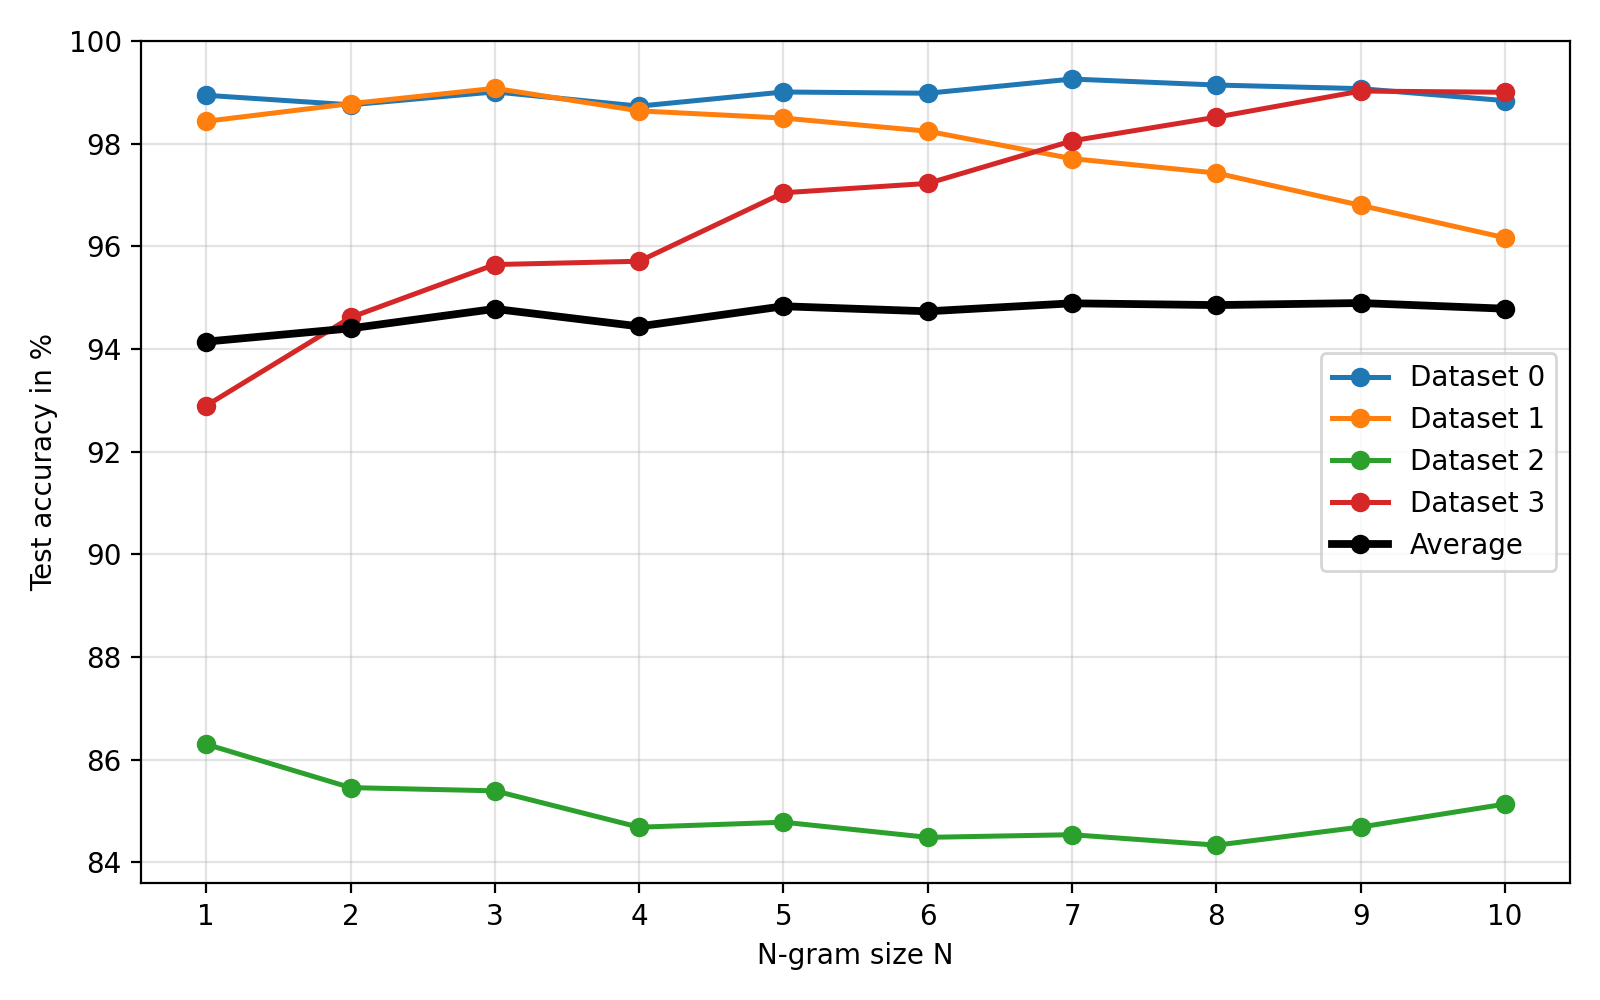
\includegraphics[width=\textwidth]
    {Images/ngram.png}
    \caption{Mean classification accuracy of the baseline HDC model for different N-gram sizes. The vector dimension is fixed to $D=10{,}000$, the number of CCIM levels to $L=40$, and uniform quantization is used. The reported accuracies are averaged over the four datasets and five seeds.}
    \label{fig:ngram}
\end{figure}
%python3 analysis/ngram_size_sweep/plot_ngram_accuracy.py --min-ngram 1 --max-ngram 10






 
Table~\ref{tab:baseline_accuracy} shows the accuracy of the baseline HDC model with $D=10{,}000$ and $L=40$. Between datasets, clear differences are apparent. Datasets~0 and~1 achieve the highest accuracies, depending on the seed, while Dataset~2 consistently performs worst. Ledwig \cite{ledwig_vdl-implementierung_2025} analyzed the datasets with PCA and concluded that these differences emerge from the data itself, because in Dataset 2, samples from different classes show a strong overlap and are thus not clearly distinguishable. 

Some variation is also visible across the different seeds. As described above, this results from the different \ac{RNG} initializations used to generate the \ac{CCIM}. The last column of Table \ref{tab:baseline_accuracy} shows the mean and standard deviation across all seeds. This mean across seeds is used in the following experiments as the main metric for the dataset. The maximum difference between seeds is below 1.1 percentage points for all datasets, and the standard deviation ranges from 0.22 to 0.43 percentage points. On average across all datasets, the model achieves 94.781\% accuracy with $L=40$ and $D=10{,}000$ dimensions, which will serve as a reference point for later evaluation.



\begin{table}[htbp]
    \centering
    \caption{Classification accuracy of the baseline HDC model for each dataset and seed. The final column reports the mean and sample standard deviation across the five runs.}
    \label{tab:baseline_accuracy}
    \begin{tabular}{c c c c c c c}
        \toprule
        \textbf{Dataset}
        & \textbf{Seed 1}
        & \textbf{Seed 2}
        & \textbf{Seed 3}
        & \textbf{Seed 4}
        & \textbf{Seed 5}
        & \textbf{Mean $\pm$ SD} \\
        \midrule
        0 & 98.96\% & 98.96\% & 99.19\% & 99.31\% & 98.62\% & 99.01\% $\pm$ 0.27\% \\
        1 & 99.08\% & 99.08\% & 99.42\% & 98.85\% & 98.96\% & 99.08\% $\pm$ 0.22\% \\
        2 & 85.37\% & 85.02\% & 85.83\% & 85.14\% & 85.60\% & 85.39\% $\pm$ 0.33\% \\
        3 & 95.51\% & 95.97\% & 95.16\% & 96.20\% & 95.39\% & 95.65\% $\pm$ 0.43\% \\
        \bottomrule
    \end{tabular}
\end{table}
Figure~\ref{fig:baseline_dimension_sweep} shows the classification accuracy of the baseline model for vector dimensions from $D=201$ to $D=20{,}000$ at a fixed number of $L=40$ \ac{CCIM} levels. Since no measured accuracy falls below $70\%$, the y-axis is limited to the range from $70\%$ to $100\%$. The vector dimension is evaluated in steps of 100 below $D=1{,}000$, 500 between $D=1{,}000$ and $D=10{,}000$, and 1,000 from $D=10{,}000$ to $D=20{,}000$.
\begin{figure}[htbp]
    \centering
    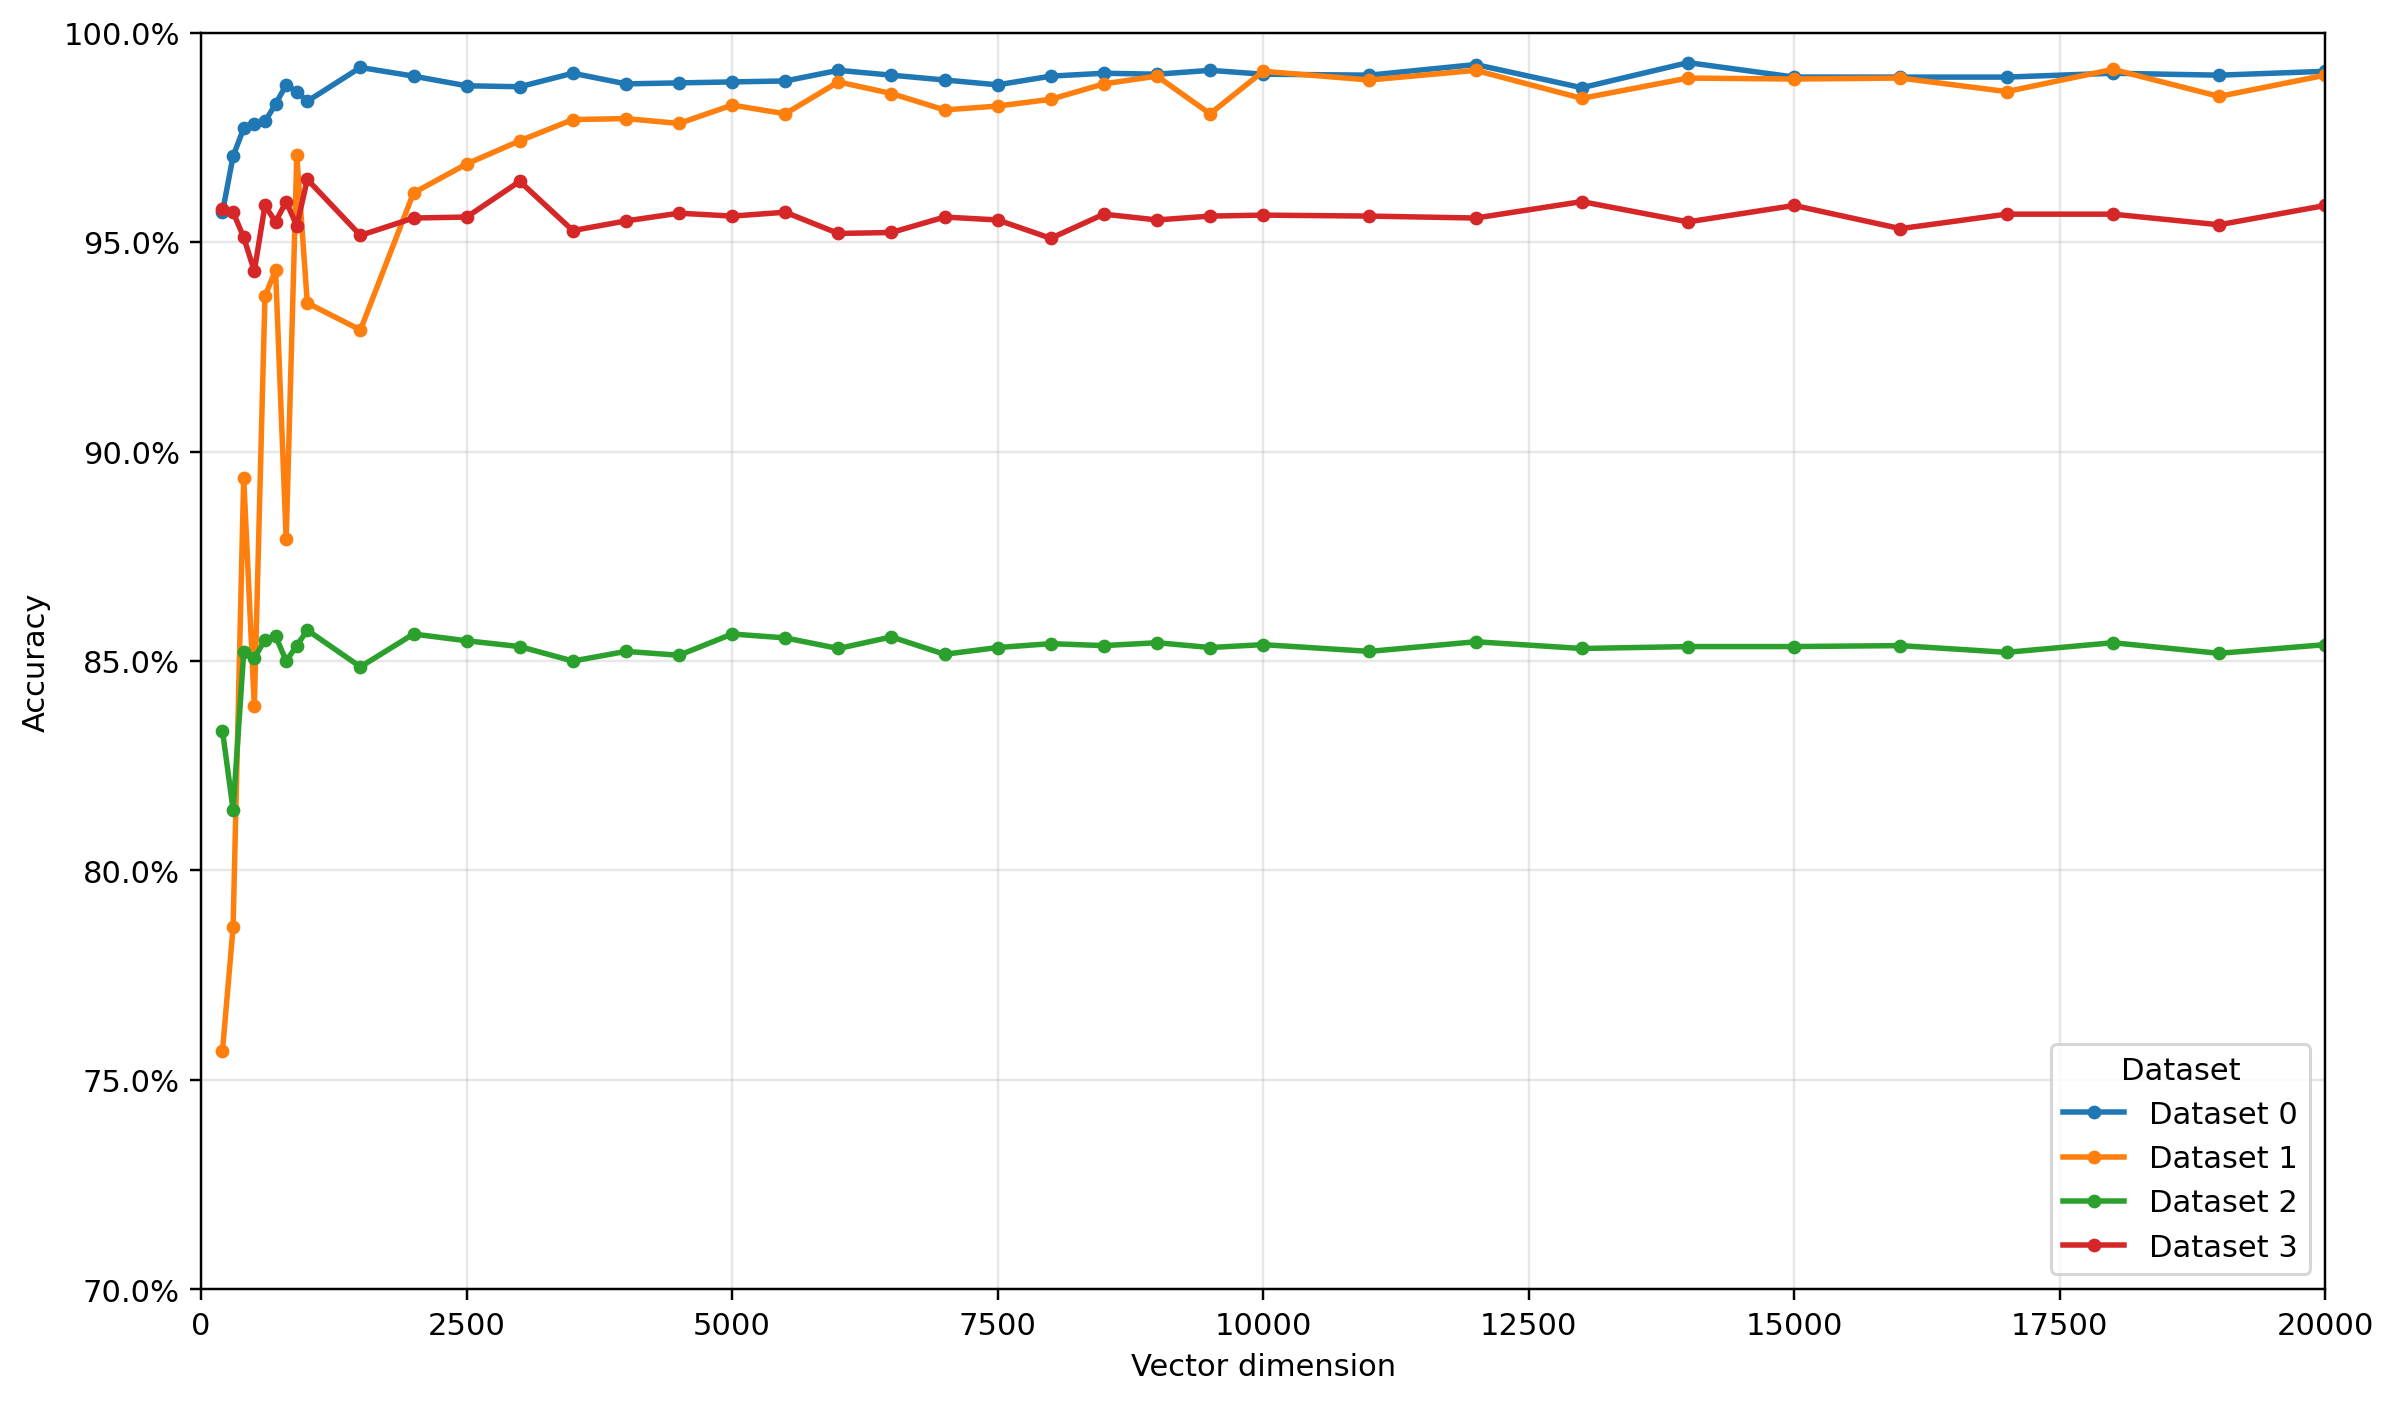
\includegraphics[width=\textwidth]
    {Images/baseline_lvl40_full.png}
    \caption{Classification accuracy of the baseline HDC model at vector dimensions from $D=201$ to $D=20{,}000$ with $L=40$ for each dataset.}
    \label{fig:baseline_dimension_sweep}
\end{figure}%python3 analysis/benchmarking/baseline/scripts/plot_accuracy_by_dimension.py --num-levels 40 --min-dimension 0 --max-dimension 20000 --output Images/baseline_lvl40_full.png
Despite the large differences in absolute accuracy across datasets, a clear trend is visible within each dataset. While low dimensions generally result in lower accuracy, the accuracy initially increases with $D$ and then saturates, such that further increases in the vector dimension provide little additional improvement. This saturation behavior also supports the choice of $D=10{,}000$ as the baseline vector dimension in this work. Comparing $D=10{,}000$ with $D=20{,}000$ shows an average accuracy increase of only 0.052 percentage points across all four datasets. The largest increase is observed for Dataset~0 with $+0.069$ percentage points, while Dataset~1 even shows a slight decrease of $0.092$ percentage points. Therefore, increasing the dimension beyond $D=10{,}000$ increases the dimension-dependent computational effort while providing only a negligible accuracy improvement on average.

On the other hand, halving the vector dimension to $D=5{,}000$ approximately halves the hypervector storage and the computational effort of operations that scale linearly with $D$. However, the average accuracy is only $0.19$ percentage points lower, with the largest decrease of $0.81$ percentage points for Dataset~1, while Dataset~2 even shows a slight increase of $0.25$ percentage points. This suggests that reducing the vector dimension by a factor of two can substantially reduce vector-dependent memory and computation while causing only a small loss in average classification accuracy. Whether \ac{CCIM} optimization and quantization can compensate for this accuracy loss at lower vector dimensions is investigated in Chapters~\ref{sec:GA_results} to~\ref{sec:combined_results}.

Figure~\ref{fig:baseline_dimension_low} shows the same experiment as Figure~\ref{fig:baseline_dimension_sweep}, but at a higher resolution of 20 dimensions and a focus on low vector dimensions from $D=201$ to $D=5{,}000$. At low vector dimensions, even small changes in $D$ can result in significant fluctuations in classification accuracy. As the vector dimension approaches $D=5{,}000$, these fluctuations become smaller. This behavior is consistent with the increased redundancy of higher-dimensional representations, in which individual dimensions have less influence on the overall representation.

The accuracy degradation at very low vector dimensions is again strongly dataset-dependent. As shown in Figure~\ref{fig:baseline_dimension_low}, the accuracies of Datasets~0, 2, and 3 at $D=1{,}000$ remain close to those at $D=5{,}000$. Datasets~2 and 3 even perform slightly better at $D=1{,}000$, while Dataset~0 performs slightly worse, but all three differences remain below one percentage point. Dataset~1, in contrast, shows a decrease of $4.72$ percentage points when reducing the vector dimension from $D=5{,}000$ to $D=1{,}000$. Below $D=1{,}000$, only Dataset~3 mostly preserves its accuracy, with a decrease of only $0.71$ percentage points at $D=201$. The other datasets show larger accuracy losses, with Dataset~1 being affected most strongly. Consequently, the dataset-average accuracies at $D=201$ and $D=1{,}000$ are $87.63\%$ and $93.54\%$, respectively, corresponding to decreases of $7.15$ and $1.24$ percentage points relative to the $D=10{,}000$ baseline.

\begin{figure}[htbp]
    \centering
    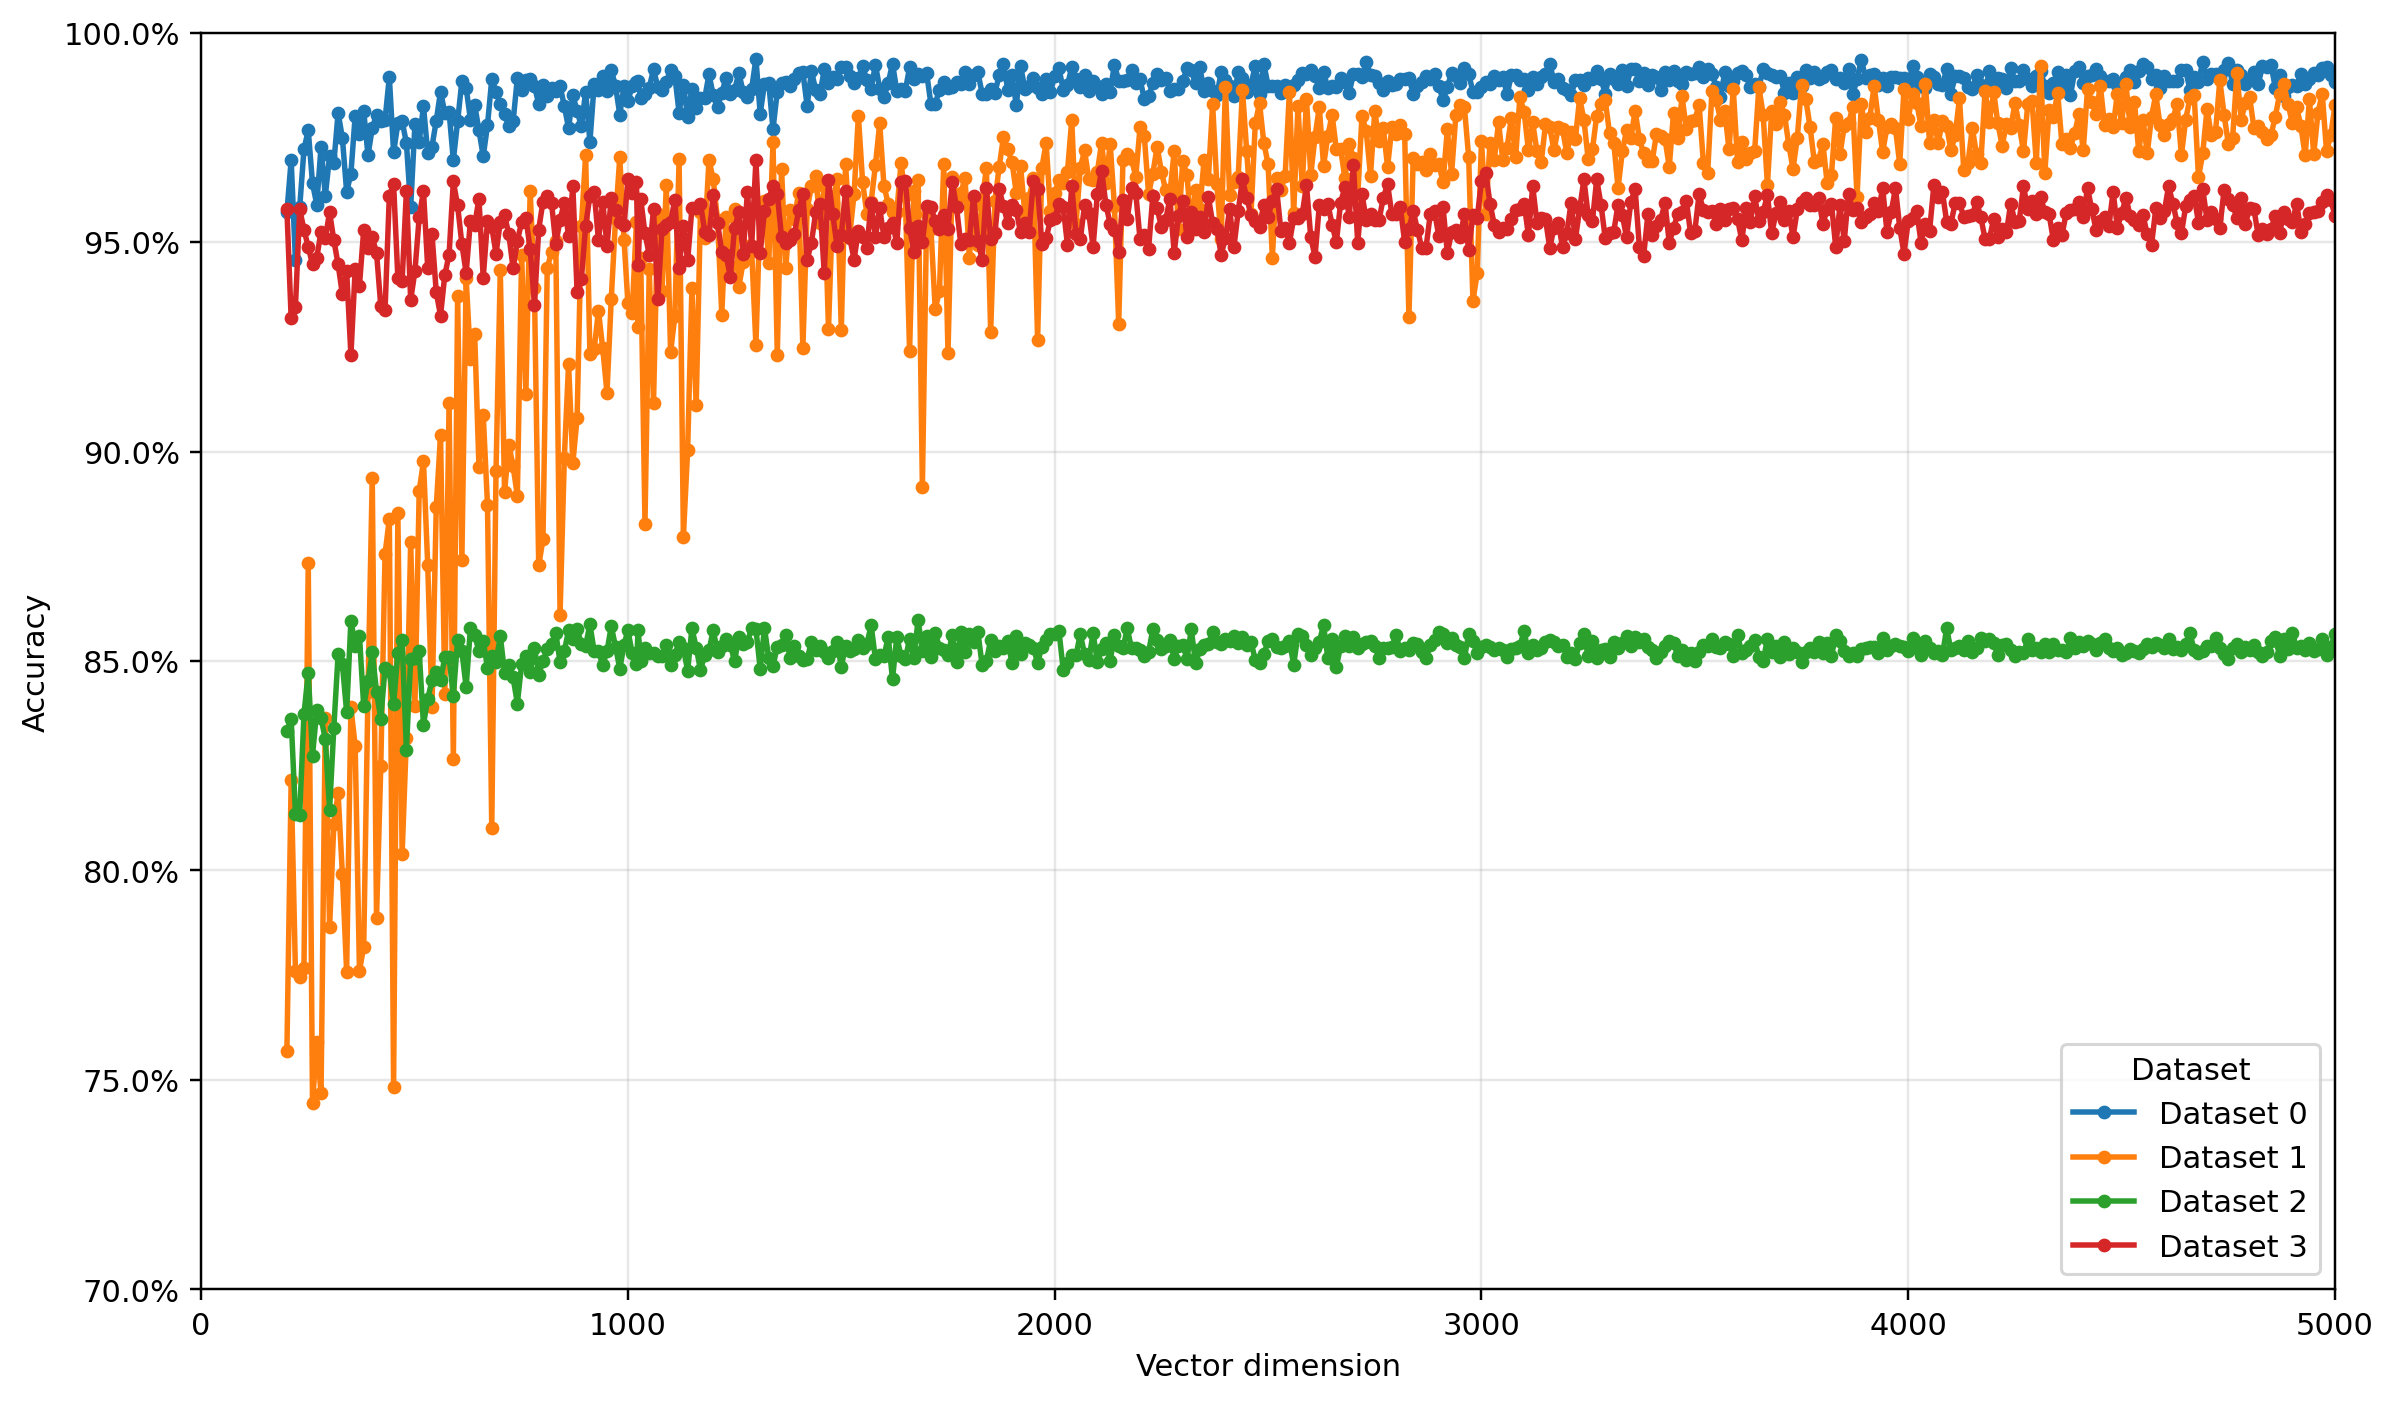
\includegraphics[width=\textwidth]
    {Images/baseline_lvl40_lowDims.png}
    \caption{Classification accuracy of the baseline HDC model at low vector dimensions with $L=40$ for each dataset.}
    \label{fig:baseline_dimension_low}
\end{figure}%python3 analysis/benchmarking/baseline/scripts/plot_accuracy_by_dimension.py --num-levels 40 --min-dimension 0 --max-dimension 5000 --dimension-grid all --output Images/baseline_lvl40_lowDims.png

%numlevels sweep
Figure~\ref{fig:baseline_levels} shows the classification accuracy as a function of the number of \ac{CCIM} levels from $L=5$ to $L=200$ at a fixed vector dimension of $D=10{,}000$. For small numbers of levels, the accuracy decreases for all datasets, as the coarse quantization provides insufficient resolution to represent relevant variations in the feature values. For Datasets~0 and 2, this degradation is mainly observed below approximately $L=13$ and $L=12$, respectively, while for Dataset~3 it extends to approximately $L=26$. For Datasets~0, 2, and 3, the accuracy eventually reaches a region in which further increases in $L$ provide little or no systematic improvement. The specific number of quantization levels $L$ of this point differs between datasets. For Datasets~0 and 2 it occurs at approximately $L=30$, while for Dataset~3 it occurs at approximately $L=64$. Between those regions, the accuracy varies nonlinearly with $L$. This suggests that the placement of the uniform quantization thresholds interacts with the feature distributions, such that some level counts may align better with discriminative regions of the data than others.
Dataset 1 is a strong outlier here. Its accuracy varies nonlinearly across the tested level counts, with local maxima around $L=40$, $L=100$, and $L=160$. This strong dependence on $L$ suggests that Dataset~1 is particularly sensitive to the alignment of the quantization thresholds and is therefore an important target for quantization optimization. In contrast to the other datasets, no comparable high-accuracy saturation region is observed. An extended experiment up to $L=500$ (not shown) further showed that the accuracy obtained at $L=40$ was not reached again at larger level counts.

\begin{figure}[htbp]
    \centering
    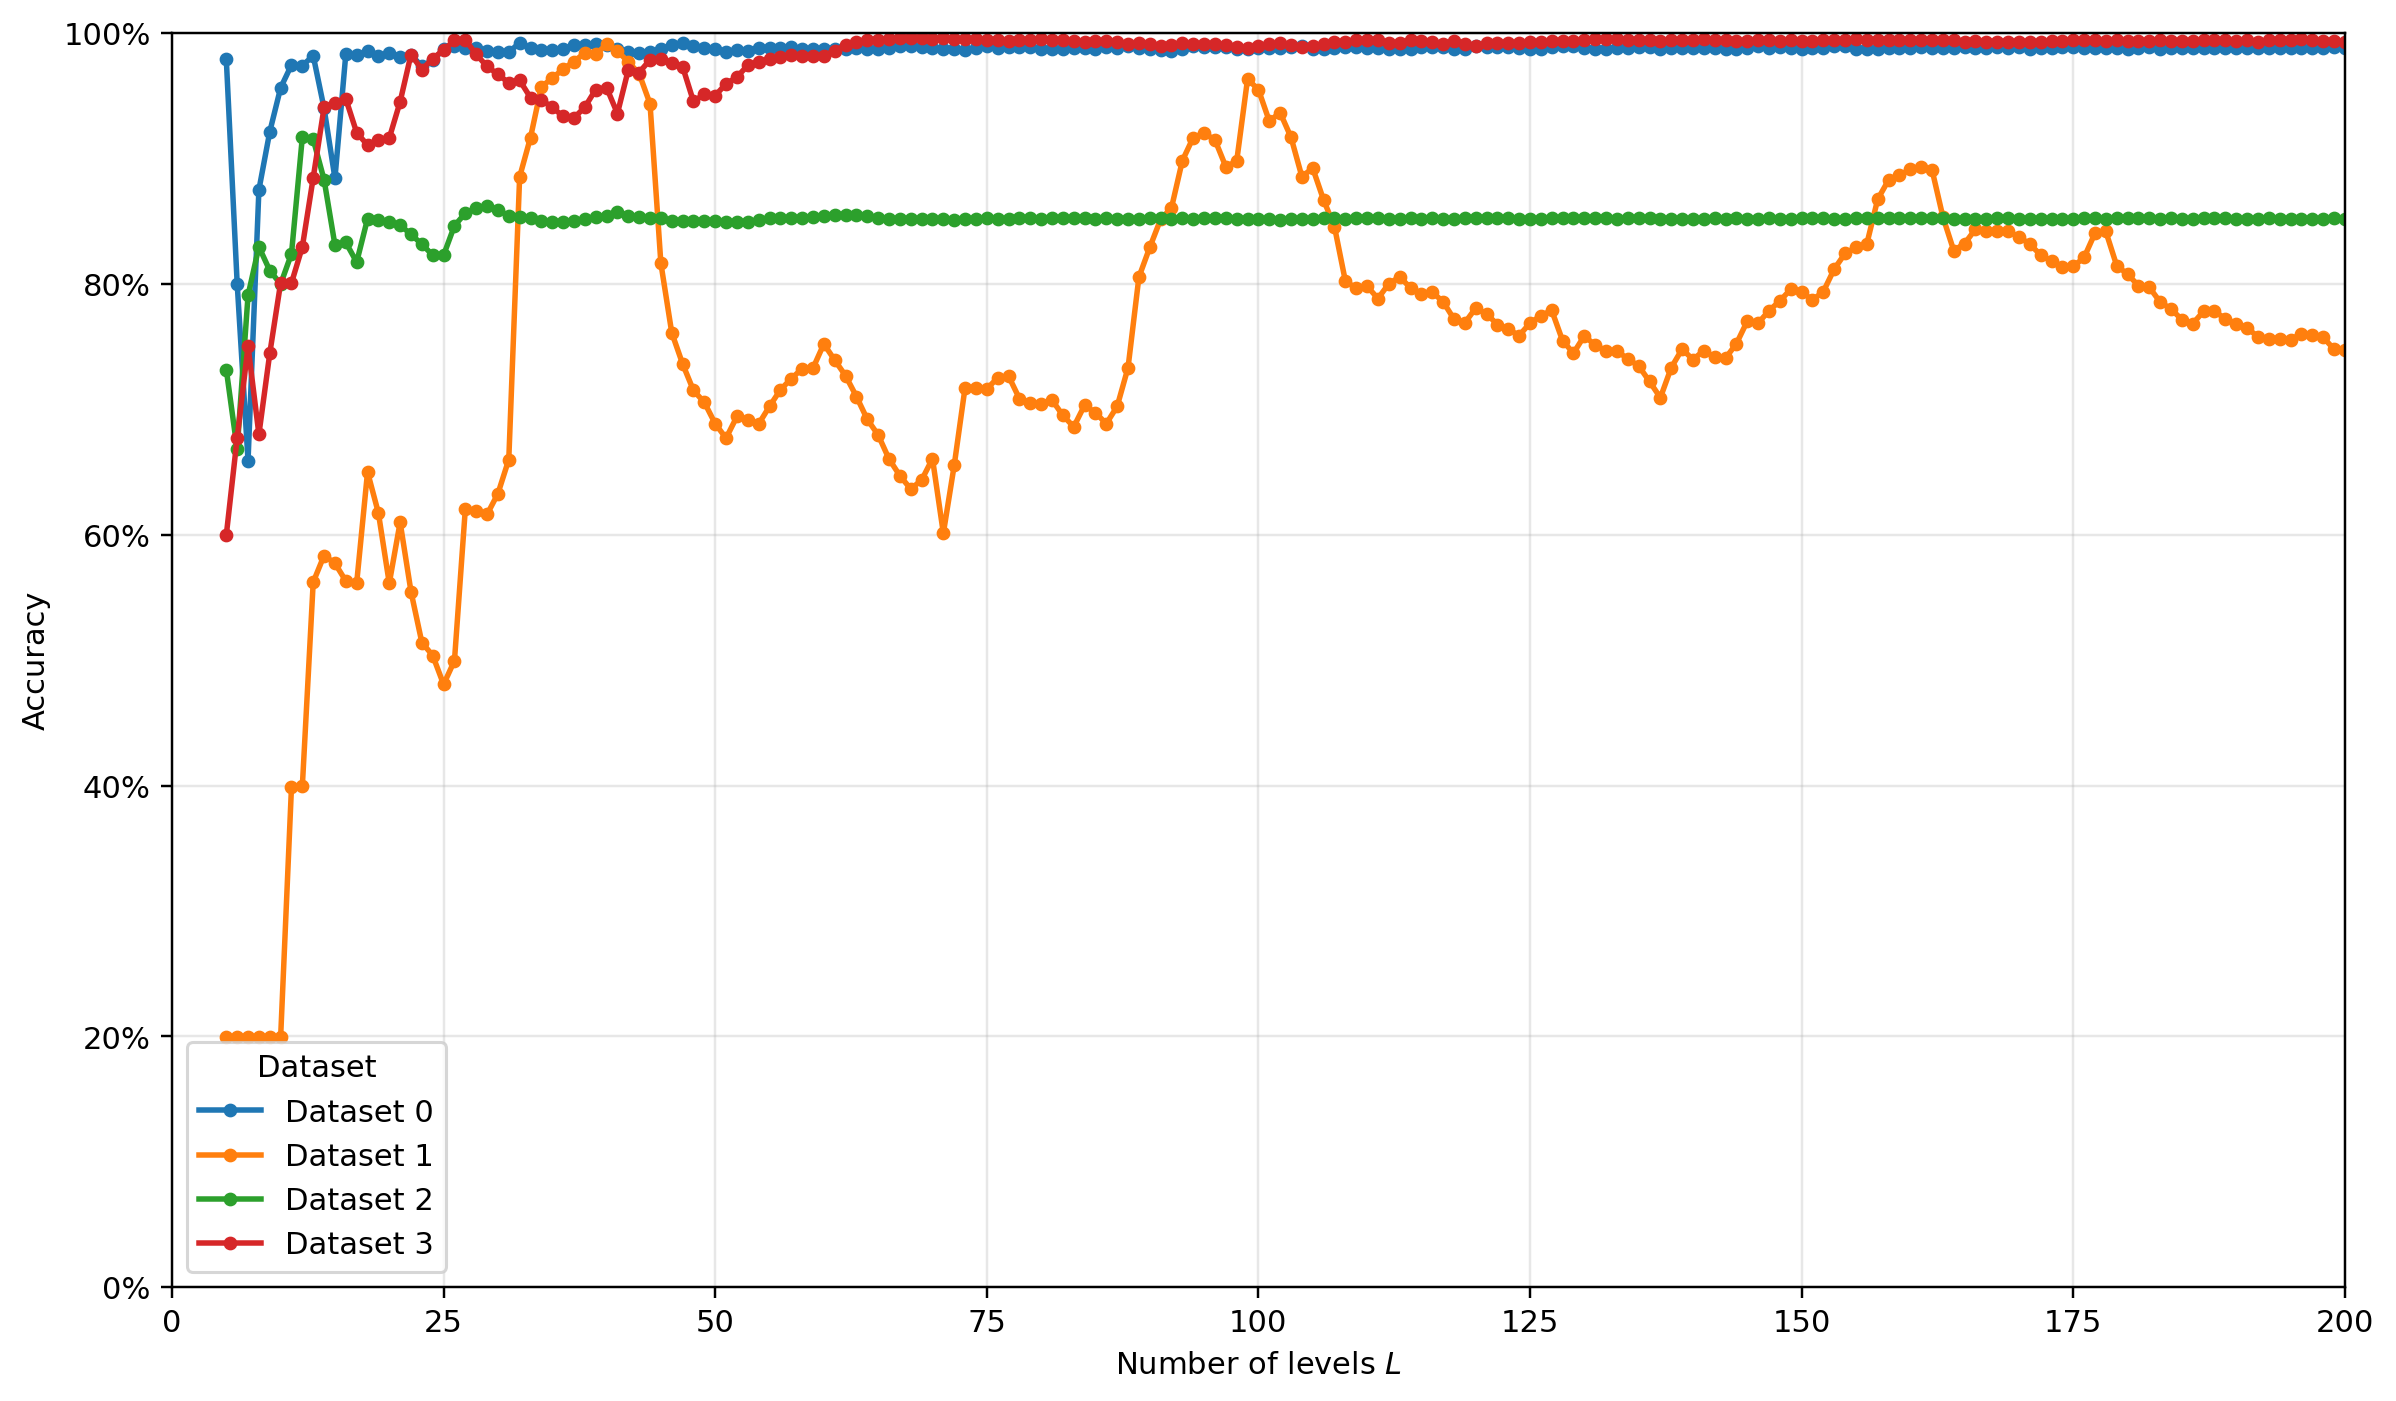
\includegraphics[width=\textwidth]
    {Images/baseline_dim10k_full.png}
    \caption{Classification accuracy of the baseline HDC model for different numbers of \ac{CCIM} levels at $D=10{,}000$.}
    \label{fig:baseline_levels}
\end{figure}

The results also show that the dependence of classification accuracy on both $D$ and $L$ is dataset-specific and nonlinear. Although increasing either parameter generally improves accuracy at low values, local maxima and saturation regions occur at different parameter values for the individual datasets. Consequently, no single tested value of $D$ or $L$ provides the best accuracy for all datasets.


\section{Results of Genetic Optimization}
\label{sec:GA_results}

The previous section showed that reducing the vector dimension can strongly reduce the model cost, but also that the baseline model loses accuracy at low dimensions. This section evaluates whether the GA-based CCIM optimization can compensate for this loss. The number of quantization levels is kept fixed at $L=40$, and uniform quantization is used, so that the distribution of the level hypervectors in the CCIM is the only changed property.

Before comparing the optimized model on the test set, the optimization process itself is analyzed. Figure~\ref{fig:ga_convergence} shows a representative convergence analysis on the example of Dataset~3 with $D=10{,}000$ averaged across five seeds. The upper plot shows the best and mean validation accuracy of the population per generation, while the lower plot shows how many newly generated individuals are selected into the next generation.

\begin{figure}[htbp]
    \centering
    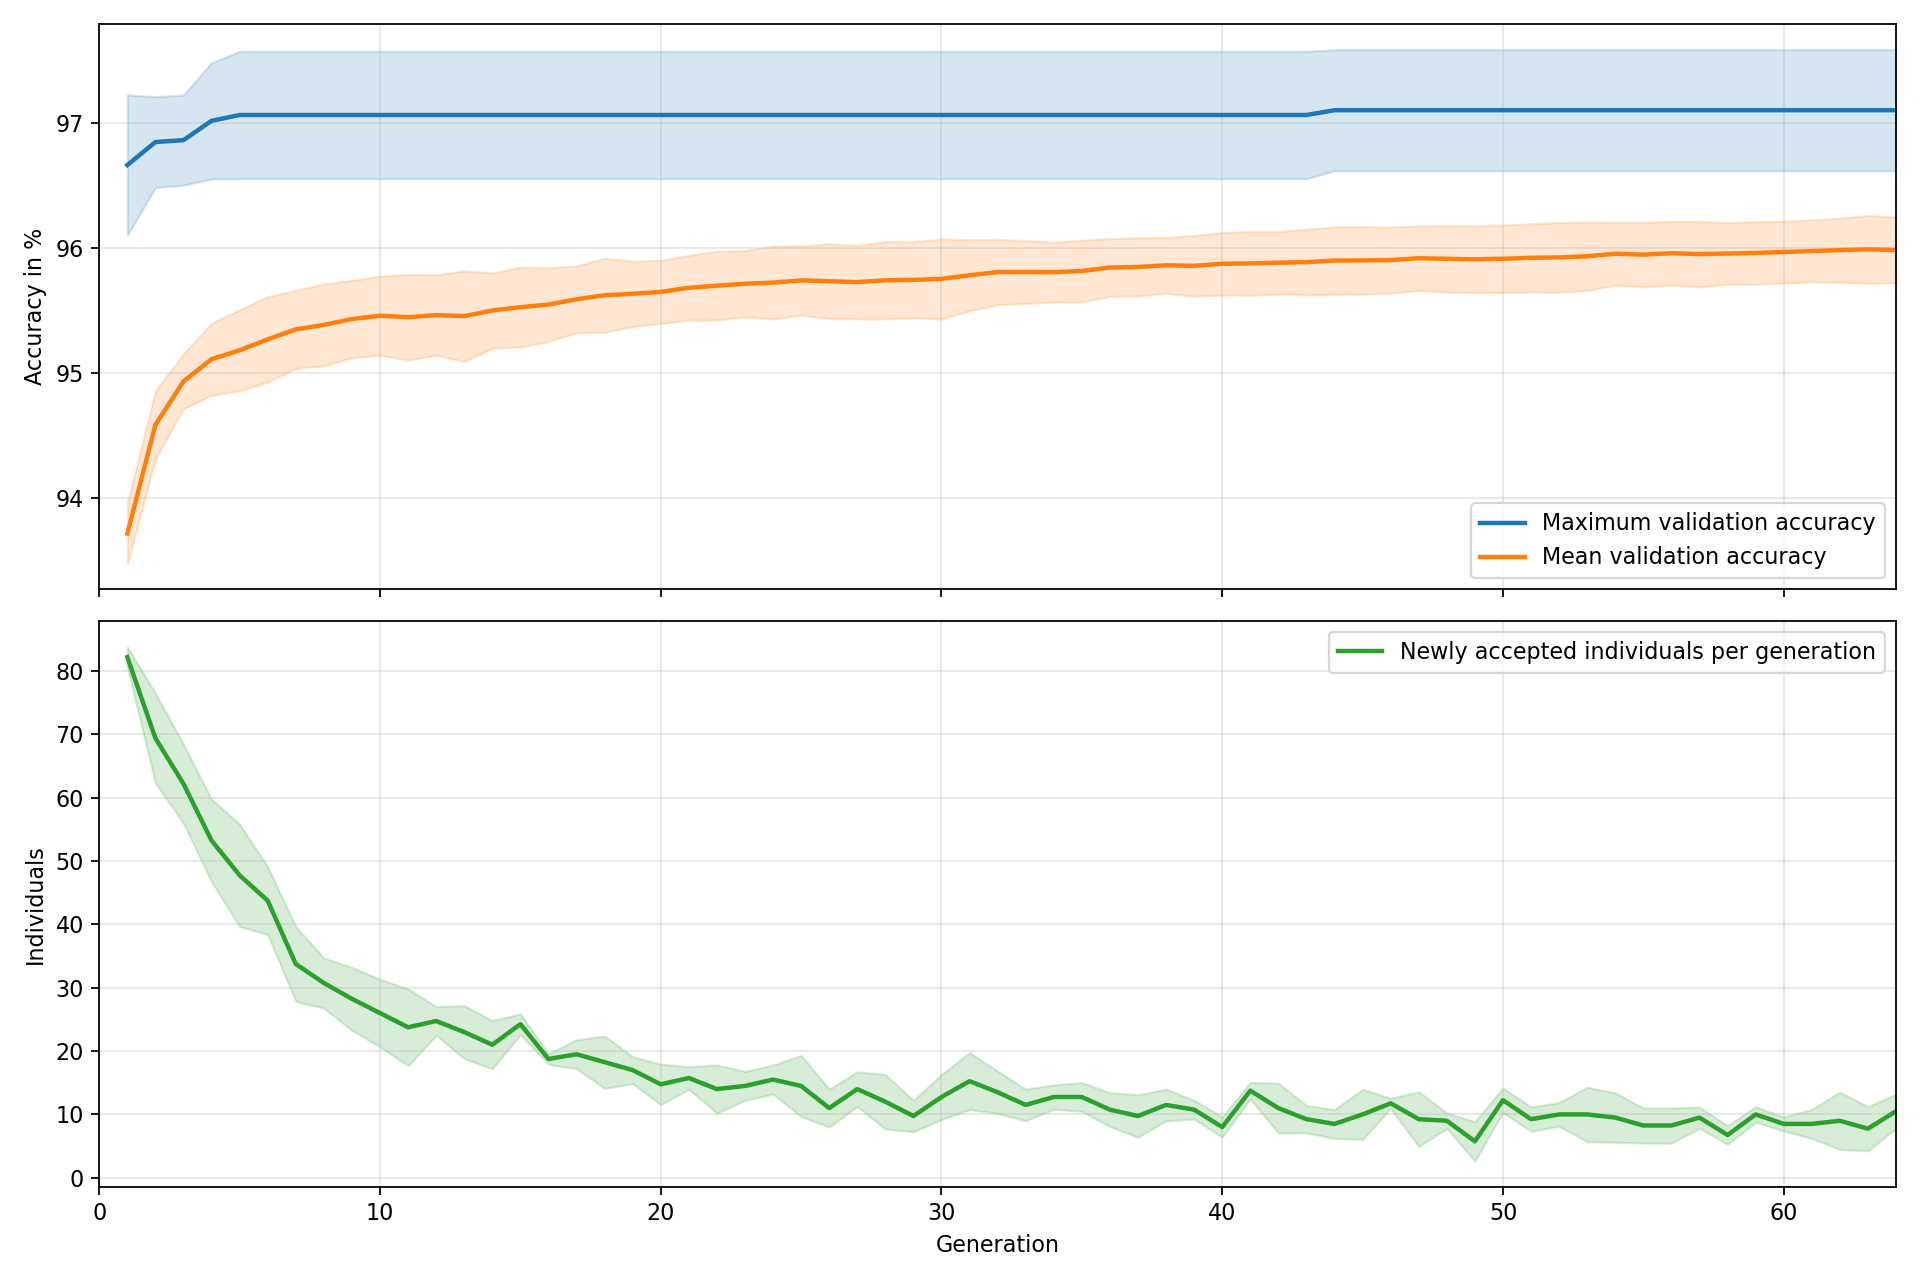
\includegraphics[width=\textwidth]
    {Images/ga_convergence.png}
    \caption{Convergence behavior of the GA-based CCIM optimization for Dataset~3 with $D=10{,}000$ and $L=40$. The upper plot shows the maximum and mean validation accuracy of the population, while the lower plot shows the number of newly accepted individuals per generation.}
    \label{fig:ga_convergence}
\end{figure}%python3 analysis/CiM_evaluation/plot_ga_run_convergence.py   --logs analysis/CiM_evaluation/dataset3_ga_cim_exports/output_dataset03_seed*_l40_d10000.txt   --show
%Dataset 3, 5 seeds, 64 gen 128 pop

The convergence behavior shows that the GA performs most of its exploration in the early generations. During this phase, many offspring are selected into the next generation, which indicates that the population still has significant room for improvement and that newly generated CCIM configurations frequently outperform existing ones. This is also reflected in the rapid increase of the best validation accuracy during the first generations.

In later generations, the optimization shifts from broad exploration to refinement. The best validation accuracy changes only minimally after the early improvement phase, while the mean population accuracy continues to increase. This indicates that the population becomes more concentrated around high-performing CCIM configurations. At the same time, the number of newly accepted individuals decreases strongly, showing that fewer offspring are selected into the next generation. Overall, the GA therefore shows as expected a clear convergence trend, while a small number of newly generated individuals is still selected in later generations.\\


To analyze how the GA actually changes the structure of the CCIM, an optimized bit-flip distribution is visualized in Figure~\ref{fig:CCIM_optimized}. It results from the final selected bit-flip matrix $\mathbf{B}^{\ast}$ for Dataset~3 and seed 1 included in the convergence analysis of Figure \ref{fig:ga_convergence}. For each transition $i$ between two neighboring level hypervectors, the plot reports how many bits are flipped. The blue lines show the feature-specific bit-flip counts, the red line shows the mean across all features, and the shaded region indicates the standard deviation across features. The dashed black line marks the equally spaced baseline.

\begin{figure}[htbp]
    \centering
    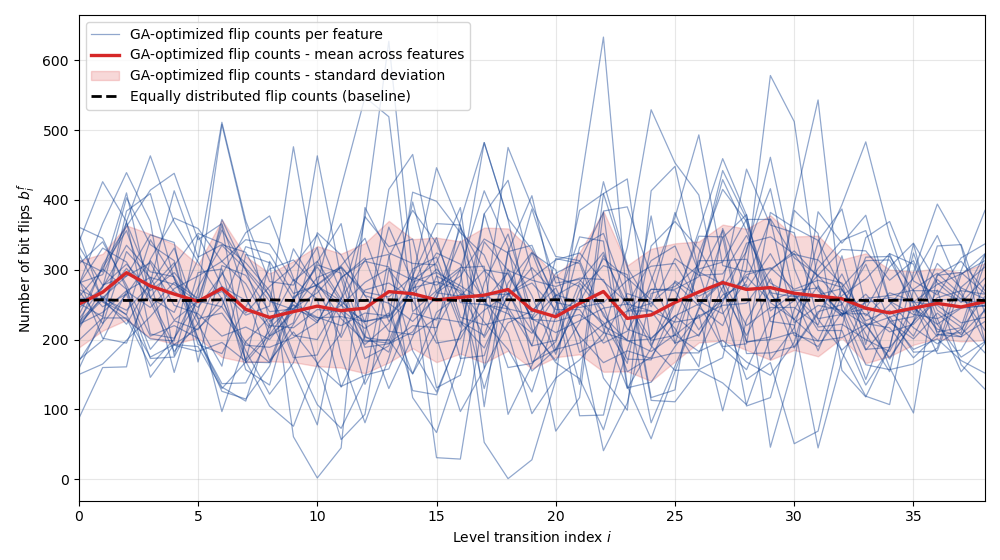
\includegraphics[width=\textwidth]
    {Images/CCIM_optimized.png}
    \caption{Optimized bit-flip distribution after GA optimization for Dataset~3. The blue lines show the feature-specific flip-count distributions, the red line shows the mean across features, and the shaded region shows the standard deviation across features. The dashed black line marks the equally spaced baseline.}
    \label{fig:CCIM_optimized}
\end{figure}
%RUN="$(basename "$(ls -td CiMs/ga_run_*dataset03_seed01_l40_d10000_pop128_gen64 | head -1)")"

%python3 analysis/CiM_evaluation/analyze_ga_cim.py \
%  --run "$RUN" \
%  --generation 64 \
%  --individual 85 \
%  --reference-cim CiMs/naive_l40_d10000_seed01/generation_0000/cim_0000.csv \
%  --show

The equally spaced baseline distributes the flip budget almost uniformly over the $L-1=39$ transitions. Since $D/(L-1)=10{,}000/39 \approx 256.41$, the baseline uses 256 or 257 bit flips per transition. The optimized CCIM preserves the same total flip budget for every feature by construction. Consequently, the mean number of bit flips across the $L-1=39$ transitions of each feature remains approximately $256.41$.

This redistribution is highly feature-specific. Across all feature-transition pairs, the optimized bit-flip counts range from 1 to 633, with a standard deviation of 79.70. In contrast, the transition-wise mean across features remains much closer to the baseline, ranging only from 230.34 to 295.78 bit flips. This indicates that the GA does not reveal a global shift that affects all features in the same way. Instead, high and low bit-flip counts occur at different transitions for different features, so no simple global pattern, such as consistently larger distances at early or late transitions, is visible.

The optimized CCIM is, in summary, structurally different from the equally spaced baseline. Some neighboring levels are compressed to almost identical hypervectors, while other neighboring levels are separated by more than twice the baseline distance. Whether this modified CCIM geometry improves the final model performance is evaluated in the following analysis.\\

%Robustness:
Since the \ac{GA} jointly optimizes validation accuracy and class-vector similarity, the final population contains multiple non-dominated solutions representing different trade-offs between the two objectives. To analyze whether the robustness objective is meaningful beyond the validation set, the individuals on the first Pareto front of the final generation are additionally evaluated on the test set.

Table~\ref{tab:ga_pareto_front} summarizes this analysis for Dataset~3, seed 1, with $D=10{,}000$ and $L=40$. The Pareto front is constructed by maximizing the validation class-average accuracy and minimizing the class-vector similarity. Lower similarity corresponds to larger separation between the learned class vectors and is therefore used as a robustness-oriented objective.

\begin{table}[htbp]
    \centering
    \small
    \setlength{\tabcolsep}{4pt}
    \caption{First Pareto front of the final GA generation for Dataset~3, seed 1, with $D=10{,}000$ and $L=40$. For each individual, the table reports the class-vector similarity, validation accuracy, test accuracy, and the difference between test and validation accuracy.}
    \label{tab:ga_pareto_front}
    \begin{tabular}{c c c c c}
        \toprule
        \textbf{Individual} 
        & \textbf{Similarity} 
        & \textbf{Validation acc.} 
        & \textbf{Test acc.} 
        & \textbf{Test $-$ Val.} \\
        \midrule
        119 & 0.313 & 95.21\% & 97.00\% & +1.78 pp \\
        82  & 0.318 & 95.44\% & 97.24\% & +1.78 pp \\
        98  & 0.319 & 95.68\% & 97.35\% & +1.66 pp \\
        71  & 0.319 & 95.99\% & 97.47\% & +1.47 pp \\
        92  & 0.321 & 96.06\% & 97.35\% & +1.28 pp \\
        73  & 0.322 & 96.22\% & 97.93\% & +1.70 pp \\
        70  & 0.325 & 96.60\% & 98.04\% & +1.43 pp \\
        69  & 0.329 & 96.60\% & 98.16\% & +1.55 pp \\
        108 & 0.331 & 96.99\% & 98.16\% & +1.16 pp \\
        85  & 0.337 & 97.22\% & 98.27\% & +1.05 pp \\
        \bottomrule
    \end{tabular}
\end{table}

Within this Pareto front, the two objectives reveal a clear trade-off. Candidates with lower class-vector similarity show a larger improvement from validation to test accuracy. The Pearson correlation between similarity and the test-validation difference is $-0.803$, with a Spearman correlation of $-0.806$. This indicates that, among Pareto-optimal individuals, stronger class-vector separation is associated with a larger gain on unseen test data.

But at the same time, lower similarity does not directly lead to the highest absolute test accuracy. The correlation between similarity and absolute test accuracy is positive, with a Pearson correlation of $0.911$. This is caused by the structure of the Pareto front. Individuals with higher validation accuracy also tend to have higher test accuracy, even if their class-vector similarity is larger. Candidate~119 represents the robustness-oriented end of the front, with the lowest similarity and one of the largest test-over-validation gains, while Candidate~85 represents the accuracy-oriented end, with the highest validation and test accuracy.

Therefore, class-vector similarity provides a useful criterion within this Pareto front, as it exposes solutions with different trade-offs between validation accuracy and class-vector separation. However, it should not replace validation accuracy as the primary objective but rather be interpreted as a secondary criterion that helps expose alternative robust solutions within the final Pareto front.

Since this analysis is performed on one representative final Pareto front, the observed correlations should be interpreted as evidence for the usefulness of the similarity objective in this experiment rather than as a general proof of robustness for all datasets and configurations.

After analyzing the optimization process and the resulting CCIM structure, the final effect of the GA optimization is evaluated on the test set. Figure~\ref{fig:ga_only_comparison} compares the classification accuracy of the HDC model with a GA-optimized CCIM against the unoptimized equally spaced CCIM for different vector dimensions at $L=40$. The red curves show the test accuracy after GA optimization, while the blue curves show the corresponding unoptimized baseline. The dotted horizontal line marks the reference accuracy of the unoptimized model with $D=10{,}000$ and $L=40$.

\begin{figure}[htbp]
    \centering
    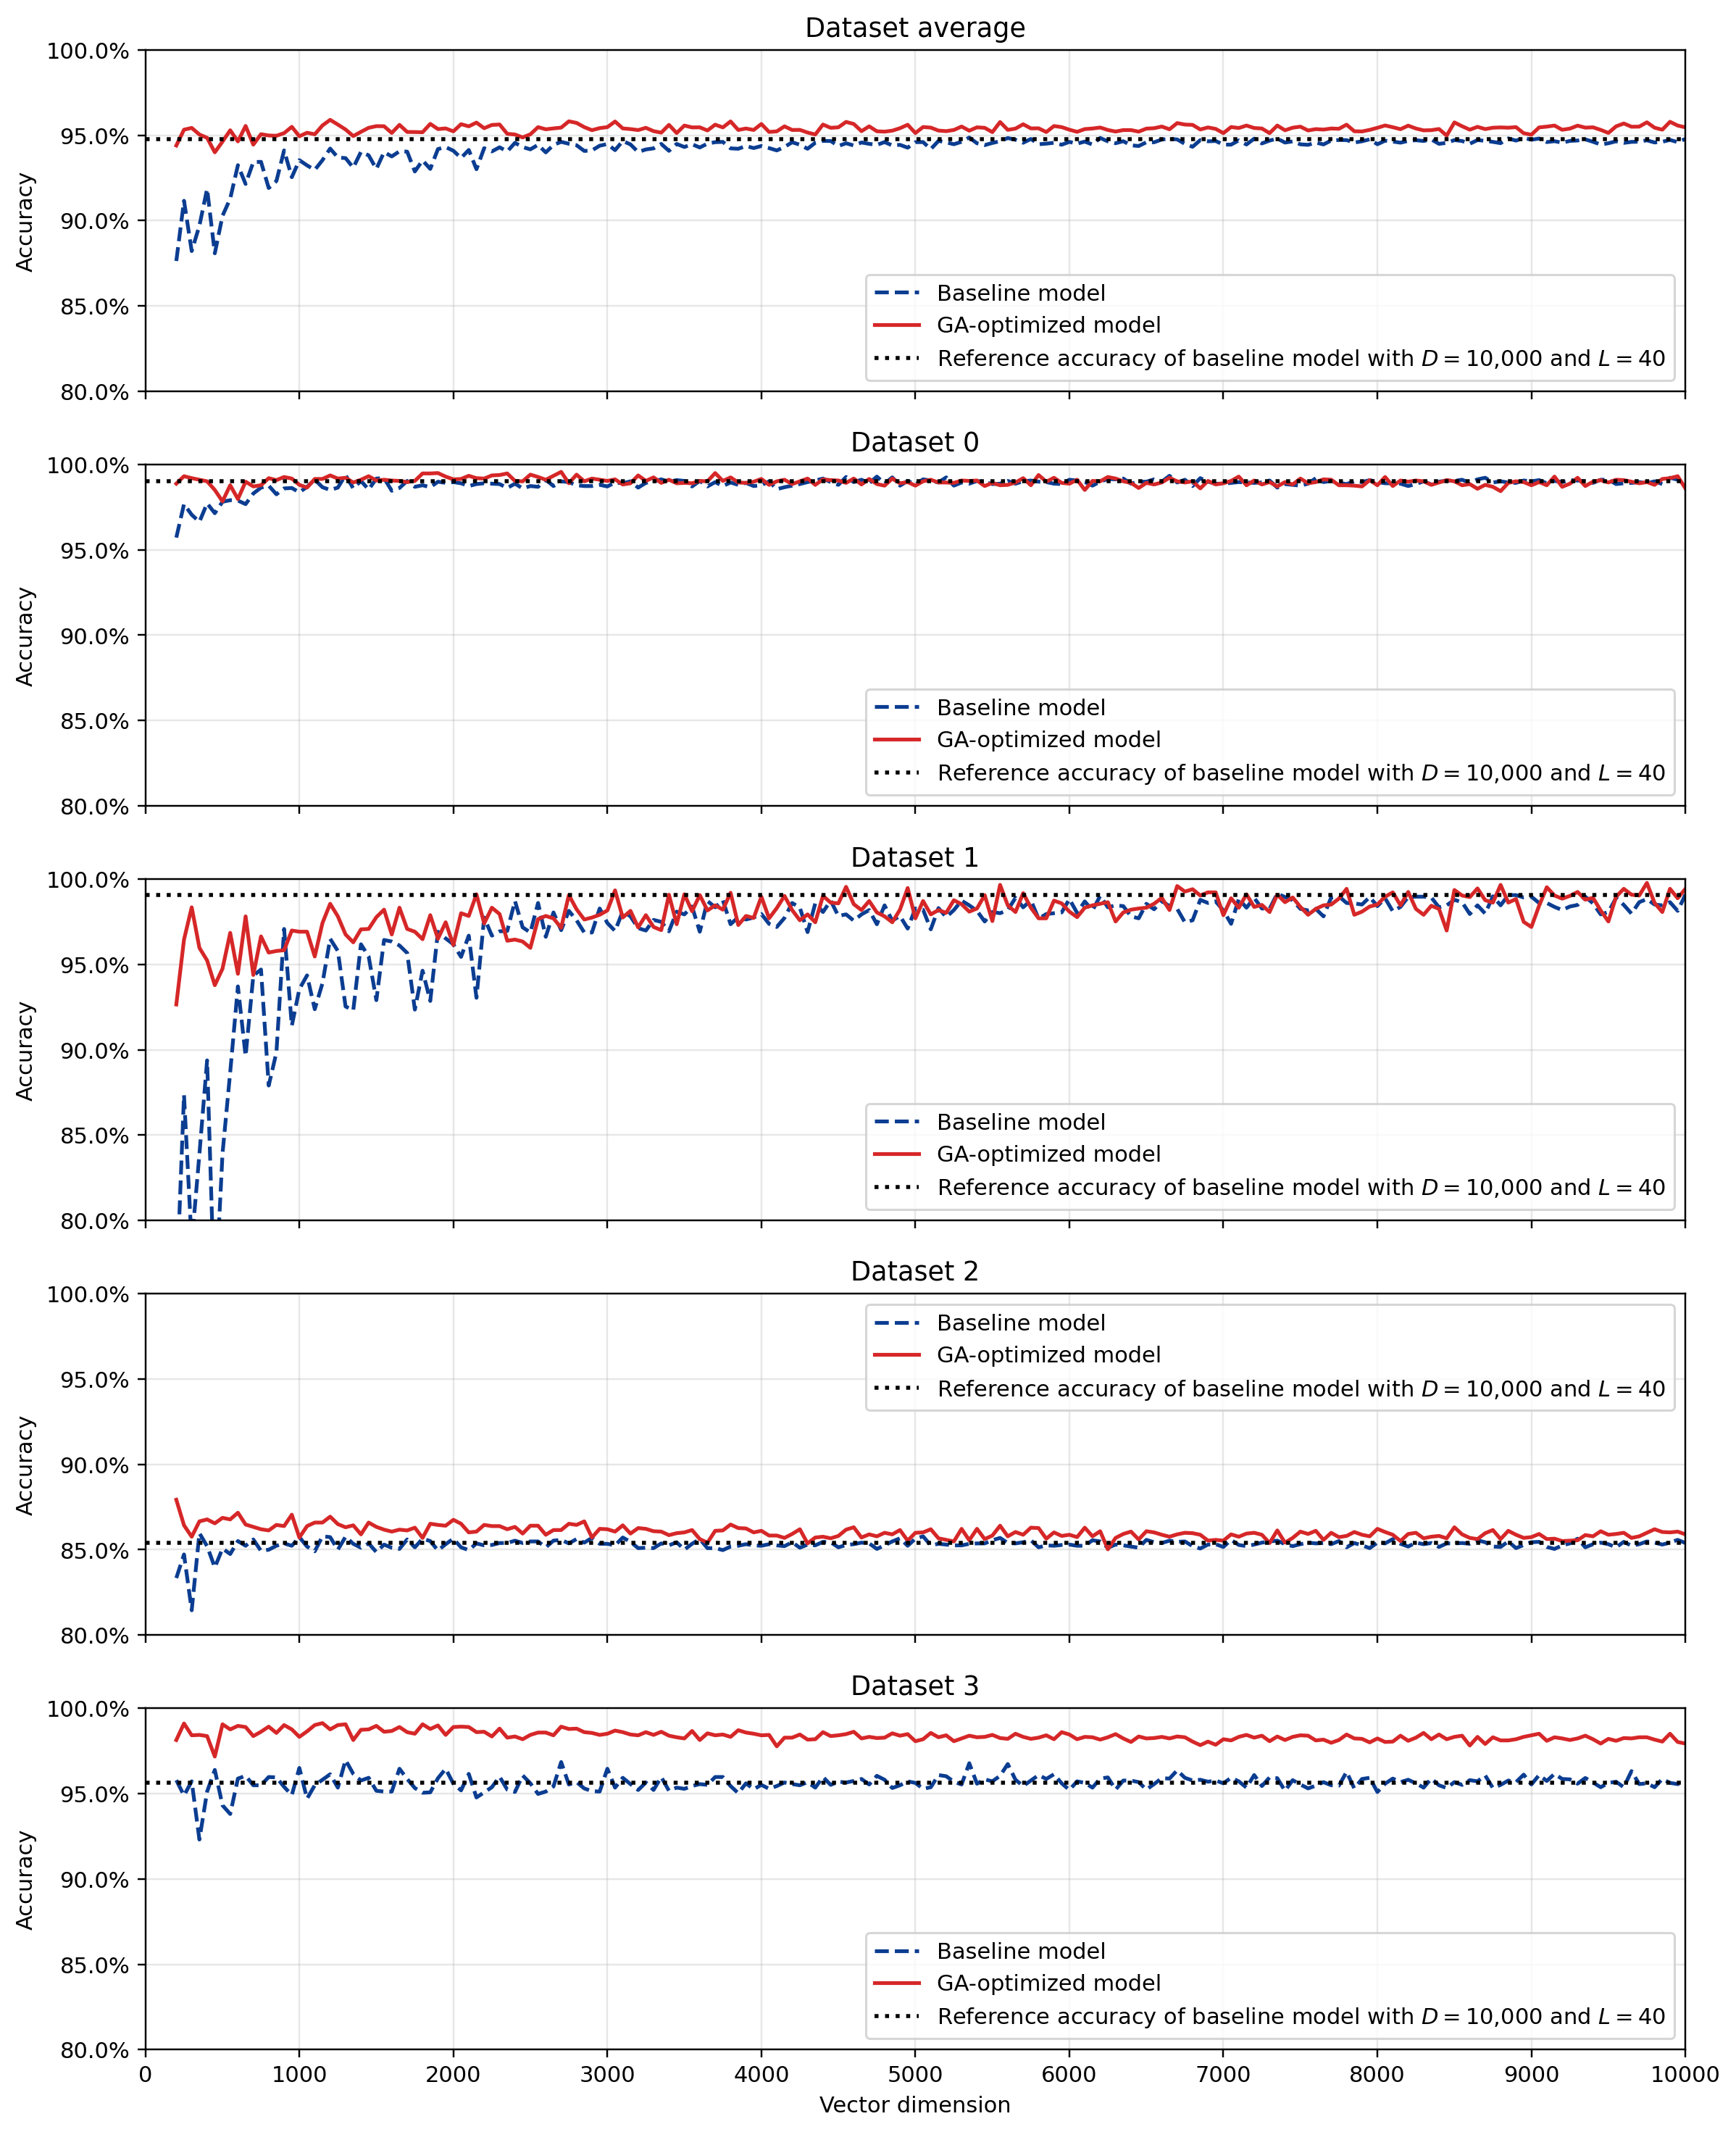
\includegraphics[width=\textwidth]
    {Images/ga_only_comparison.png}
    \caption{Test accuracy of the GA-optimized CCIM (red) compared with the unoptimized equally spaced CCIM (blue) for different vector dimensions at $L=40$. The dotted horizontal line marks the reference accuracy of the unoptimized model with $D=10{,}000$ and $L=40$.}
    \label{fig:ga_only_comparison}
\end{figure} %python3 analysis/benchmarking/GA_only/scripts/plot_pre_vs_post_by_dimension.py --num-levels 40 --min-dimension 0 --max-dimension 10000 --y-min 0.8 --y-max 1.0

\begin{table}[htbp]
    \centering
    \caption{Selected dataset-average test accuracies from the GA-only dimension sweep. The reference is the unoptimized model with $D=10{,}000$ and $L=40$, which achieves $94.78\%$.}
    \label{tab:ga_dimension_summary}
    \begin{tabular}{c c c c c}
        \toprule
        \textbf{$D$}
        & \textbf{Unoptimized}
        & \textbf{GA-optimized}
        & \textbf{Gain}
        & \textbf{GA vs. reference} \\
        \midrule
        201    & 87.63\% & 94.40\% & +6.76 pp & -0.39 pp \\
        251    & 91.16\% & 95.32\% & +4.16 pp & +0.54 pp \\
        501    & 90.28\% & 94.63\% & +4.35 pp & -0.16 pp \\
        701    & 93.43\% & 94.45\% & +1.02 pp & -0.33 pp \\
        751    & 93.44\% & 95.06\% & +1.62 pp & +0.28 pp \\
        1,000  & 93.54\% & 94.94\% & +1.40 pp & +0.16 pp \\
        1,024  & 93.00\% & 95.96\% & +2.96 pp & +1.18 pp \\
        1,050  & 93.23\% & 95.14\% & +1.91 pp & +0.36 pp \\
        10,000 & 94.78\% & 95.46\% & +0.68 pp & +0.68 pp \\
        \bottomrule
    \end{tabular}
\end{table}

The dataset-average result in the top plot of Figure~\ref{fig:ga_only_comparison} and in Table~\ref{tab:ga_dimension_summary} shows that the GA-optimized CCIM improves the test accuracy over the unoptimized CCIM across the evaluated dimension range. The improvement is largest at low dimensions, where the baseline model loses the most accuracy. At $D=201$, the GA increases the dataset-average test accuracy from $87.63\%$ to $94.40\%$, but this still remains slightly below the reference at 94.78\%. Therefore, $D=201$ is still too small if the original reference accuracy should be preserved.

The dataset-average curve exceeds the high-dimensional reference at some low dimensions, but these early crossings are not stable. For example, the optimized model is above the reference at $D=251$, but falls below it again at $D=501$ and $D=701$. Therefore, the first crossing is not used as the selection criterion. Instead, the relevant point is the first dimension after which all larger measured dimensions remain above the reference.
With this criterion, the empirical stability threshold is $D=751$. From this point onward, all larger evaluated dimensions remain above the reference. \\

The dataset-specific plots show that the dataset-average result is not achieved uniformly across all datasets. For Dataset~0, the baseline and reference are already close to saturation at about $99\%$. Consequently, the GA cannot substantially improve the result, but it keeps the reduced-dimensional model close to the reference.

For Dataset~1, the GA improves the low-dimensional configurations substantially, from $75.69\%$ to $92.65\%$ at $D=201$ and from $93.55\%$ to $96.91\%$ at $D=1{,}000$. However, the optimized result at $D=1{,}000$ remains below the Dataset~1 reference accuracy of $99.08\%$. Thus, for this dataset, the GA optimization improves the reduced-dimensional model, but does not fully compensate for the reduction in vector dimension at $L=40$.

Datasets~2 and~3 show a stronger benefit from the GA. For Dataset~2, the GA-optimized model reaches or exceeds its reference for nearly all evaluated dimensions. But the largest improvement relative to the reference is observed for Dataset~3. Already at $D=201$, the optimized model reaches $98.13\%$, compared with the reference of $95.65\%$. Thus, for these datasets, the optimized CCIM not only compensates for reduced vector dimensions, but also improves the accuracy compared with the reference.\\

Overall, the GA-only results show that the optimized CCIM preserves the dataset-average reference accuracy from the empirical stability threshold of $D=751$ onward for all evaluated dimensions. This result does not imply that every dataset individually reaches its own high-dimensional reference, but it shows that the average accuracy can be maintained with a substantially smaller representation. For the FPGA implementation, the reduced dimension is chosen as $D=1{,}024$. Although smaller 64-bit-aligned dimensions above the threshold would also be possible, $D=1{,}024$ is selected because it results in exactly 16 words of 64 bits and provides a convenient power-of-two configuration for the hardware implementation. Compared with the original $D=10{,}000$ configuration, this reduces the hypervector size by a factor of approximately $9.8$, while keeping a margin above the measured stability threshold. Since CCIM storage, associative-memory storage, memory traffic, and the number of vector elements processed by the HDC operations scale directly with $D$, this reduction is highly relevant for the FPGA implementation.




\section{Quantization Results}
\label{sec:quantization_results}

After improving the HDC model with GA optimization and showing that the vector dimension can be reduced while maintaining the dataset-average accuracy, the second optimization approach is evaluated in this section. Instead of optimizing the CCIM hypervectors themselves, this approach changes the quantization boundaries used to map continuous feature values to discrete CCIM levels, as described in Section \ref{sec:quantization}.

As a baseline, uniform binning is used, as in the baseline model and in the previous GA experiments. The method is described in Section~\ref{sec:UniformBinning}. For comparison, the four additional quantization methods described in Sections~\ref{sec:quantileBinning} to~\ref{sec:ChiBinning} are applied. The goal is to adapt the level boundaries so that the resulting levels represent the feature values more meaningfully. If this allows the same accuracy to be reached with fewer levels, the size of the CCIM can be reduced.\\

Before comparing the classification accuracy, the learned quantization boundaries are analyzed directly. Figure~\ref{fig:quantization_threshold_example} shows one example for Dataset~0, feature~15, seed~1, and $L=40$. The upper plot shows for each quantization method at which feature value the level transition boundaries are placed. The lower plot illustrates the value distribution of the feature on which the quantizers are fitted. The grey histogram shows all samples across $L=40$ uniformly spaced bins, while the black curve shows the corresponding \ac{CDF}. In addition, the samples and the \ac{CDF} are shown separately for each class, using one color per class and dashed lines for the class-wise \acp{CDF}.


\begin{figure}[htbp]
    \centering

    % Dataset 0
    \begin{minipage}[t]{0.99\textwidth}
        \centering
        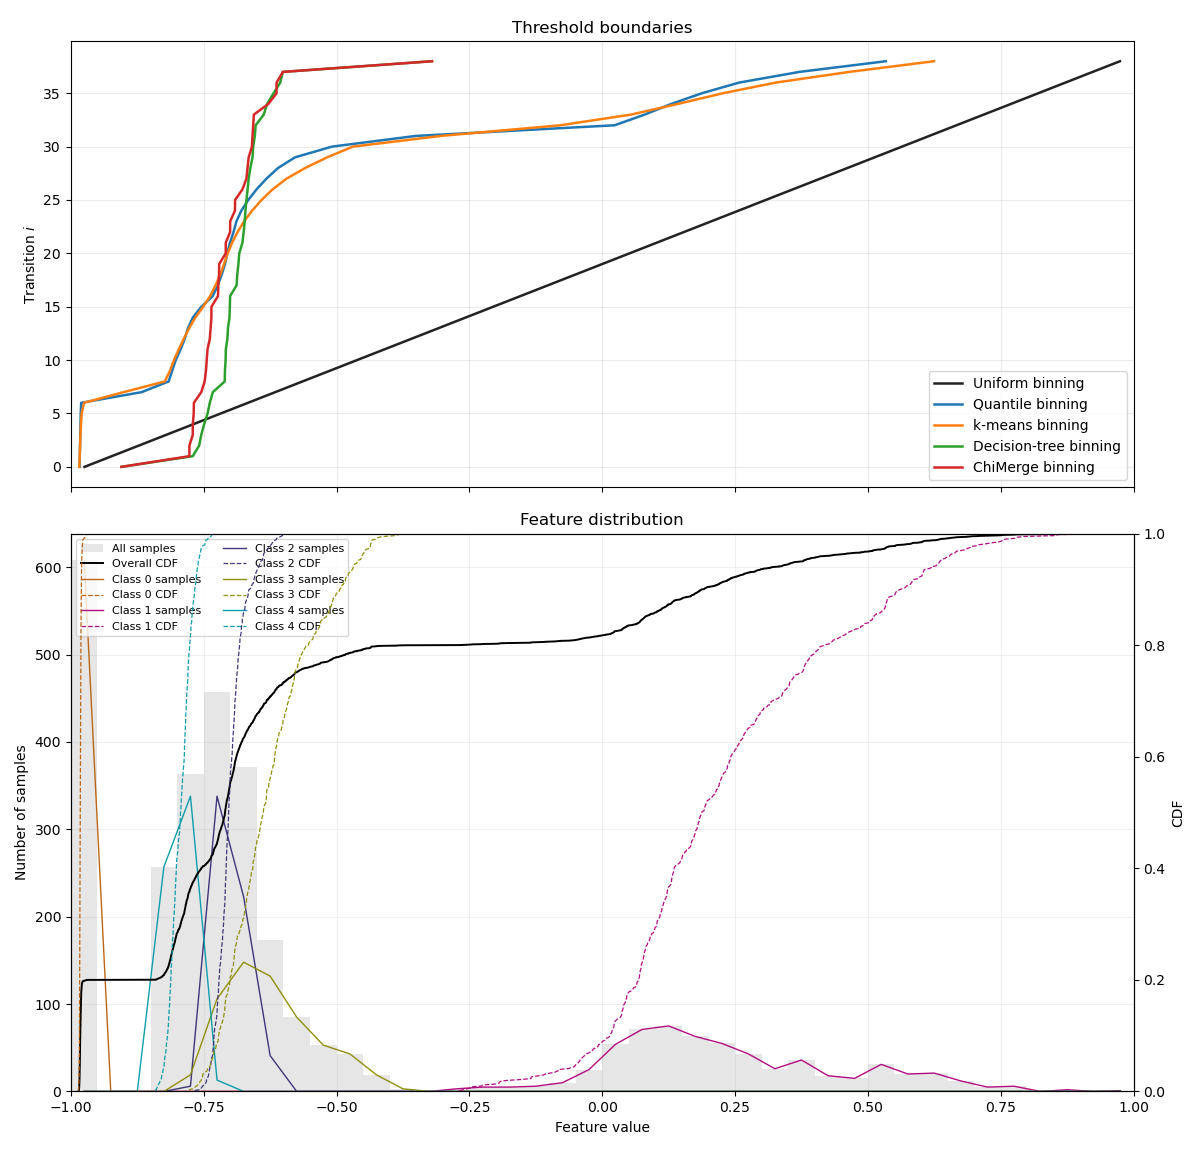
\includegraphics[width=\linewidth]
        {Images/quantizer_histogram.png}
        
    \end{minipage}
    

    \caption{Quantization thresholds and feature-value distribution for Dataset~0, feature~15, seed~1, and $L=40$. The upper plot shows the threshold positions of the different quantization methods. The lower plot shows the corresponding feature distribution, separated by class.}
    \label{fig:quantization_threshold_example}
\end{figure}
%python3 analysis/benchmarking/quantizer_only/threshold_analysis/scripts/plot_thresholds_with_histogram.py \
  %--dataset 0 \
  %--feature 15 \
  %--seed 1 \
  %--num-levels 40 \
  %--vector-dimension 10000 \
  %--methods all

  The feature distribution is strongly non-uniform. Although the histogram range is $[-1,1]$, most samples are concentrated in the negative part of the range. Class~0 forms a very narrow cluster close to $-0.98$, Classes~2, 3, and~4 overlap strongly in the range around $-0.8$ to $-0.6$, and Class~1 is separated from the other classes and extends mainly to values above -0.3 and into the positive range.

This structure explains the different threshold placements of the quantization methods.
Uniform binning distributes the boundaries evenly over the full input range, so the transition thresholds are linearly spaced with respect to the absolute feature value.
Quantile and k-means binning adapt to the sample distribution instead. Since both methods are unsupervised, their threshold distributions are very similar. Both methods concentrate more thresholds in regions with a high sample density, as expected from their dependence on the value distribution. As a result, their thresholds cover a smaller effective value range than uniform quantization. However, the unsupervised methods also assign a considerable part of their thresholds to values above -0.3, which corresponds to the distribution of the samples, but is not necessarily useful for separating the classes in this feature, since this region mainly contains Class~1.

Decision-tree binning and ChiMerge behave differently, because they use the class labels during threshold selection. Both methods place their thresholds only between approximately $-0.90$ and $-0.32$. This means that the class-pure outer regions are not subdivided further, because the samples of Class~0 are mapped below the first threshold, and the samples of Class~1 are mapped above the last threshold. Instead, the available thresholds are concentrated in the region where Classes~2, 3, and~4 overlap and are therefore harder to separate. Thus, the supervised quantizers do not primarily approximate the full feature distribution, but focus their boundaries on class-relevant intervals.

This example shows that adaptive quantization can strongly change the value representation before HDC encoding. However, a more data-adaptive or class-aware threshold distribution does not automatically imply better final accuracy. Therefore, the following experiments evaluate whether these modified boundaries improve the complete HDC classifier.


Figure~\ref{fig:quantizer_level40} compares the different quantization methods for a fixed number of levels $L=40$ and varying vector dimension. The blue dashed curve shows uniform binning as the baseline, while the red, orange, green, and purple curves show quantile binning, k-means binning, decision-tree binning, and ChiMerge binning, respectively. The black dotted line marks the reference accuracy of the uniform baseline model with $D=10{,}000$ and $L=40$. The experiments are evaluated on the test set and averaged over seeds 1 to 5. The plotted dimensions range from $D=201$ to $D=10{,}000$, with a finer spacing of 50 below $D=1{,}000$ and a spacing of 100 dimensions above $D=1{,}000$.


\begin{figure}[htbp]
    \centering
    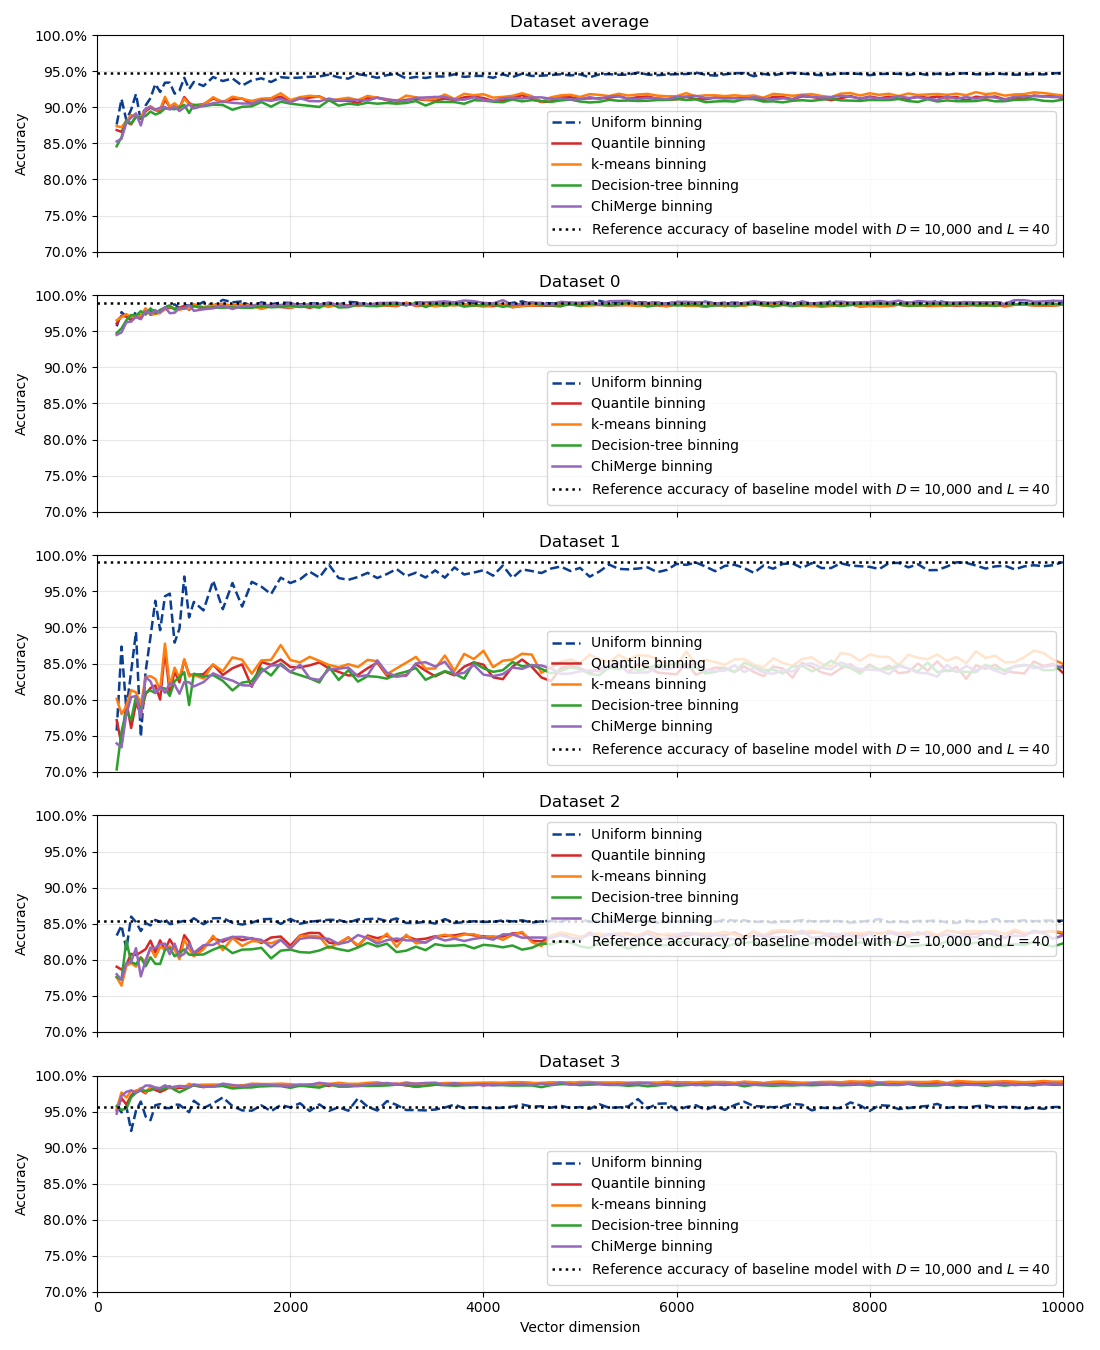
\includegraphics[width=\textwidth]
    {Images/quantizer_only_comparison40.png}
    \caption{Test accuracy of different quantization methods for $L=40$ and varying vector dimension. Uniform binning is shown as the blue dashed baseline. The black dotted line marks the reference accuracy of the uniform baseline model with $D=10{,}000$ and $L=40$.}
    \label{fig:quantizer_level40}
\end{figure}
%python3 analysis/benchmarking/quantizer_only/scripts/plot_pre_vs_baseline_by_dimension.py --num-levels 40 --min-dimension 0 --max-dimension 10000 --y-min 0.7 --y-max 1.0

The results show that the effect of adaptive quantization is highly dataset-dependent. 
For Dataset~0, all methods remain close to the uniform baseline, which indicates that the baseline quantization is already sufficient and leaves little room for improvement.
For Datasets~1 and~2, advanced quantization reduces the accuracy instead of improving it. This effect is strongest for Dataset~1, where even the best adaptive configuration remains far below the uniform reference. Dataset~2 shows a smaller but consistent decrease. Thus, for these datasets, changing the quantization boundaries alone does not produce a more useful HDC representation.
Dataset~3 shows the opposite behavior. Here, all advanced quantizers clearly outperform uniform binning, with k-means binning reaching $99.17\%$ at $D=10{,}000$ compared with the uniform reference of $95.65\%$. This shows that adaptive quantization can substantially improve the HDC classifier for datasets in which the learned boundaries provide a more suitable representation of the feature values.

However, this improvement is not strong enough to compensate for the losses on the other datasets. On the dataset average, all adaptive quantizers remain below the uniform baseline at $L=40$. In addition, none of the adaptive methods reaches the reference accuracy of \(94.78\%\). Therefore, adaptive quantization alone is not sufficient as a replacement for uniform binning.\\

While the previous comparison fixed the number of levels to $L=40$ and varied the vector dimension, Figure~\ref{fig:quantizer_10k} evaluates the opposite direction. Here, the vector dimension is fixed to $D=10{,}000$, while the number of levels is varied from $L=5$ to $L=100$. This experiment tests whether adaptive quantization can reduce the required number of CCIM levels.


\begin{figure}[htbp]
    \centering
    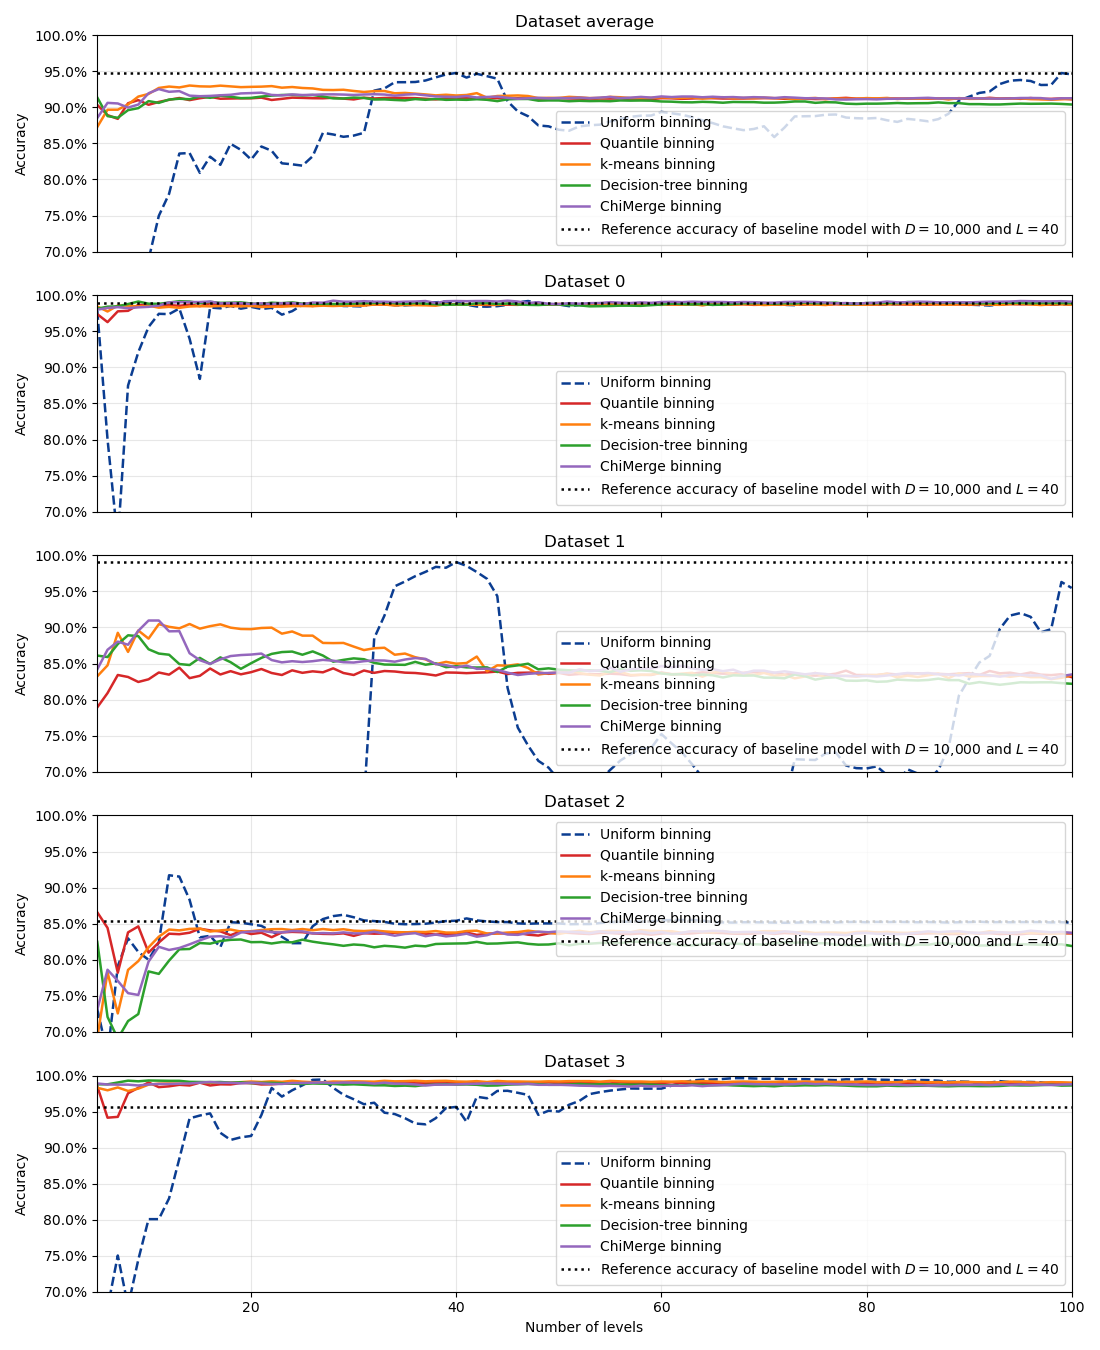
\includegraphics[width=\textwidth]
    {Images/quantizer_only_comparison10k.png}
    \caption{Test accuracy of different quantization methods for $D=10{,}000$ and varying number of levels. Uniform binning is shown as the blue dashed baseline. The black dotted line marks the reference accuracy of the uniform baseline model with $D=10{,}000$ and $L=40$.}
    \label{fig:quantizer_10k}
\end{figure}

The main difference between uniform and adaptive quantization is the dependence on the number of levels. Uniform binning varies strongly with $L$ and shows pronounced peaks and drops, especially for Datasets~1 and~3. In contrast, the adaptive quantizers are much more stable across the tested level range. This indicates that data-dependent thresholds reduce the sensitivity of the HDC model to the exact choice of $L$.

This behavior is especially useful at small numbers of levels. In the dataset average, the adaptive quantizers already reach a similar accuracy at low $L$ as they do at $L=40$, while uniform binning can be much weaker for unfavorable level counts. However, this stability is not sufficient to preserve the fixed reference accuracy. Even the best configuration on the dataset average, k-means binning with $93.04\%$ at $L=14$, remains below the uniform reference of $94.78\%$.

The dataset-specific results confirm the conclusion from the fixed-$L$ comparison in Figure \ref{fig:quantizer_level40}. Dataset~3 benefits clearly from adaptive quantization, and the adaptive methods remain above the reference over almost the entire level range. Dataset~0 is mostly insensitive to the quantization method, except very small level counts. For Datasets~1 and~2, however, adaptive quantization does not provide a reliable improvement over uniform binning. Therefore, the effect of adaptive quantization remains strongly dataset-dependent.

The comparison between the quantization methods shows that no single method is consistently superior. The differences between the methods are smaller than the differences between datasets and smaller than the gap between advanced and uniform quantization at the reference configuration. Averaged over all level counts from $L=5$ to $L=100$ at $D=10{,}000$ and over all datasets, k-means binning performs slightly best with $91.6\%$, while decision-tree binning is lowest with $90.9\%$. Quantile binning and ChiMerge lie between these values. This indicates that the main limitation is not the choice of a specific quantizer, but the fact that adaptive quantization itself is not consistently beneficial across datasets. There is also no clear advantage of supervised over unsupervised methods in this experiment.

Overall, quantization alone reduces the dependence on the exact number of levels, but it does not preserve the reference accuracy on the dataset average. Therefore, it is not sufficient as a standalone method for reducing the number of levels $L$. The result is still useful, because it shows that adaptive thresholds can stabilize configurations with small numbers of levels. The following section therefore evaluates whether this property becomes beneficial when adaptive quantization is combined with GA-based CCIM optimization.

\section{Combined Evaluation and Final Configuration}
\label{sec:combined_results}

The previous sections showed that GA optimization improves the CCIM representation, while adaptive quantization alone does not preserve the reference accuracy on the dataset average. Therefore, this section evaluates whether adaptive quantization becomes useful when combined with GA-based CCIM optimization.

Figure~\ref{fig:combined_comparison} compares the GA-optimized model with uniform binning to GA-optimized models using the four new quantization methods. The number of levels is fixed to $L=40$, while the vector dimension is varied. The dashed blue curve shows the GA-optimized model with uniform binning, the dashed grey curve shows the unoptimized uniform baseline, and the dotted black line marks the reference accuracy of the unoptimized model with $D=10{,}000$ and $L=40$.

\begin{figure}[htbp]
    \centering
    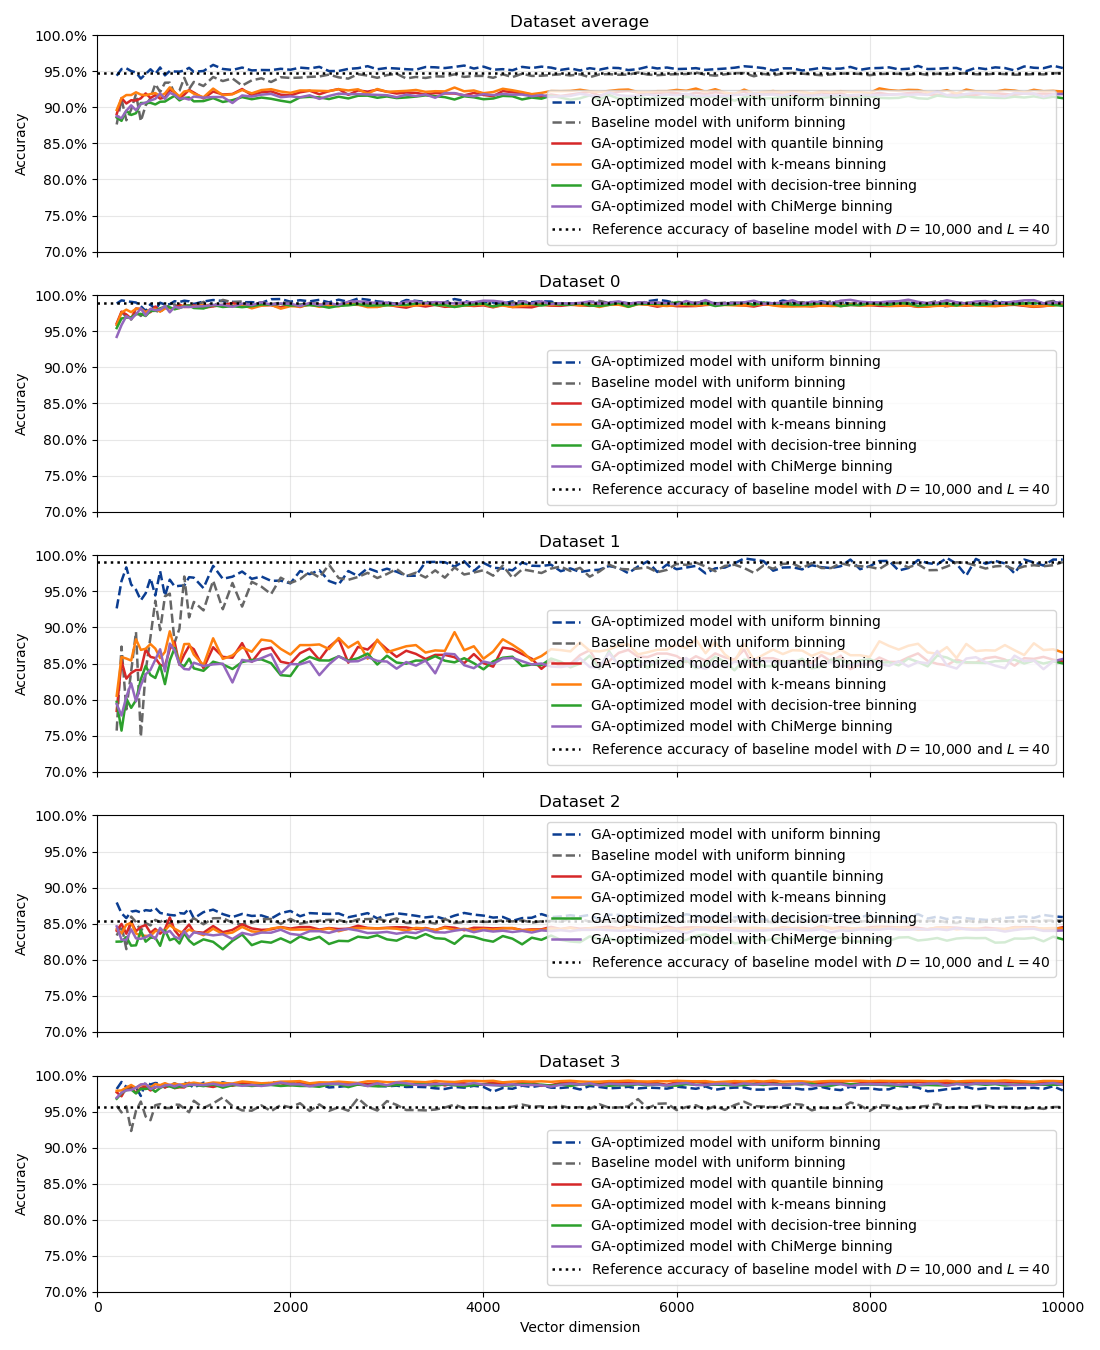
\includegraphics[width=\textwidth]
    {Images/combi_comparison.png}
    \caption{Test accuracy of GA-optimized models with uniform and adaptive quantization for $L=40$ and varying vector dimension. The dashed blue curve shows the GA-optimized model with uniform binning, the dashed grey curve the unoptimized uniform baseline, and the dotted black line the reference accuracy of the unoptimized uniform model with $D=10{,}000$ and $L=40$.}
    \label{fig:combined_comparison}
\end{figure}

The dataset-average result shows that adaptive quantization does not improve the GA-optimized model. The best-performing configuration remains GA optimization with uniform binning, reaching a best measured value of $95.90\%$ in this experiment. In contrast, all GA-optimized adaptive quantizers stay below the reference accuracy of $94.78\%$ on the dataset average. Even the best-performing adaptive combination, k-means binning with GA, reaches a maximum dataset-average accuracy of only $92.79\%$.

The dataset-specific behavior matches the quantization-only results. Dataset~3 benefits from adaptive quantization, but on average across datasets this gain is outweighed by the losses on Datasets~1 and~2. Dataset~0 shows only small differences between the methods. Thus, GA optimization does not remove the dataset dependence of adaptive quantization.

Therefore, adaptive quantization is not used for the final HDC configuration in the FPGA accelerator. Based on the dimension-reduction results in Section \ref{sec:GA_results} and the quantization analysis presented here, the configuration selected for the FPGA evaluation uses uniform binning with $L=40$, a GA-optimized CCIM, and the hardware-aligned vector dimension $D=1{,}024$.


\section{FPGA Accelerator Results}
\label{sec:FPGA_results}

After evaluating the algorithmic optimizations of the HDC model, this section evaluates the FPGA accelerator presented in Section \ref{sec:fpga_accelerator}. The goal is to determine how the optimized model maps to FPGA hardware and which trade-off between processing performance and resource usage results from different degrees of parallelism.

First, the hardware configuration is defined based on the results of the previous sections. Two accelerator variants with different degrees of word-level parallelism are then evaluated. The fully parallelized implementation represents the performance-oriented end of the design space, while the second implementation reduces word-level parallelism to decrease the hardware requirements. Both implementations use the same HDC model and accelerator pipeline, such that the influence of the hardware parallelization can be evaluated independently of the classification model. Finally, the resulting processing performance is compared with the timing requirements of the EMG application.

\subsection{Hardware Configuration}
\label{sec:hardware_config_FPGA}
%Include constants choiced based on previous results. 
% --> derive and describe bit sizes of accelerator data elements. 

The parameters used for the hardware configuration of the accelerator are derived from the results of the previous sections. The GA evaluation identified an empirical stability threshold of $D=751$, above which the dataset-average accuracy remains above the reference when using an optimized \ac{CCIM}. Since the accelerator uses words of width $W=64$ bits and requires the vector dimension to be divisible by the word width, $D=1{,}024$ is selected as a hardware-aligned dimension above the empirical stability threshold.
The number of quantization levels is kept at $L=40$. As shown in Section \ref{sec:quantization_results}, the investigated quantization methods did not preserve the reference accuracy consistently when reducing the number of levels. All other model parameters are kept from the previous sections.

This configuration also determines the widths of the accelerator data types. Representing one of $L=40$ quantization levels requires $w_{\mathrm{level}}=\left\lceil \log_2(40)\right\rceil=6$
bits, while the \(C=5\) classes require $w_{\mathrm{class}}=\left\lceil \log_2(5)\right\rceil=3$ bits. A Hamming distance for $D=1024$ can take values from 0 to 1024 and therefore requires $w_{\mathrm{distance}}=\left\lceil \log_2(D+1) \right\rceil=11$ bits.

Together with the 3-bit command type, the packed accelerator command has a width of
\[
    w_{\mathrm{cmd}}
    =
    3 + w_{\mathrm{class}} + F \cdot w_{\mathrm{level}}
    =
    3 + 3 + 32 \cdot 6
    =
    198~\mathrm{bits}.
\]
For the 32-bit AXI4-Stream interface described in Section~\ref{sec:Axi}, one command therefore requires $\left\lceil \frac{198}{32} \right\rceil=7$ AXI beats. The response consists of one validity bit and one Hamming distance for each class, resulting in

\[
    w_{\mathrm{rsp}}
    =
    1 + C \cdot w_{\mathrm{distance}}
    =
    1 + 5 \cdot 11
    =
    56~\mathrm{bits}.
\]
It is consequently transferred using $\left\lceil \frac{56}{32} \right\rceil=2$ AXI beats. 

The selected vector dimension also reduces the CCIM size compared with the original \(D=10{,}000\) configuration. The CCIM contains \(F \cdot L \cdot D\) bits and therefore requires $32 \cdot 40 \cdot 1024=1{,}310{,}720~\mathrm{bits}=163.84~\mathrm{kB}$, which is smaller by a factor of approximately $9.8$ than in the reference configuration.
The associative memory contains $C=5$ class vectors and therefore requires an additional $5 \cdot 1{,}024 = 5{,}120~\mathrm{bits} = 640~\mathrm{bytes}$.




\subsection{Fully Parallel Implementation}
\label{sec:FullyParallelResults}

To investigate the performance-oriented variant of the accelerator, the fully parallelized implementation is evaluated first.
As described in Section \ref{sec:fpga_accelerator}, the hypervectors are processed in words of 64 bits and the number of words processed in parallel determines the degree of word-level parallelism. In the fully parallelized version, all 16 words are processed in parallel during spatial encoding, class vector accumulation and Hamming distance computation. The target for HLS and FPGA implementation is the XCVU57P-FSVK2892-3-E FPGA with a target clock period of $10~\mathrm{ns}$, corresponding to a clock frequency of $100~\mathrm{MHz}$. The XCVU57P FPGA belongs to AMD's Virtex UltraScale+ HBM family and is designed for high-throughput, data-intensive applications. It provides a generous amount of hardware resources and is therefore well suited for first evaluating the maximum degree of parallelism of the accelerator without strongly restricting the architecture by device capacity \cite{amd_virtex_nodate}.

The generated RTL is verified using the complete sequence of training and inference commands. For all 870 inference samples, the responses, including the validity information and the Hamming distances for all five classes, match the expected outputs. 
The steady-state inference latency, measured from the first AXI command beat until the final AXI response beat, is $52$ clock cycles. At $100~\mathrm{MHz}$, this corresponds to a latency of $0.52~\mathrm{\mu s}$. Due to the pipelined accelerator structure, the processing of consecutive samples overlaps. After the pipeline is filled, inference results are produced at an interval of 12 clock cycles. The resulting steady-state throughput is therefore $\mathrm{TP}_{\mathrm{full}}=\frac{100~\mathrm{MHz}}{12}=8.33~\mathrm{MSamples/s}.$

Detailed stage measurements of the inference path show that the spatial encoding requires six cycles of computation. For valid N-grams, the temporal encoding requires ten cycles and the Hamming distance computation three cycles, while the response generation requires six cycles, followed by two cycles until the second AXI response beat is transferred. In steady-state operation, the spatial encoder can additionally wait up to four cycles for downstream acceptance, resulting in an observed input-to-output latency of up to ten cycles for the spatial encoding stage. Since the pipeline stages operate concurrently, these stage latencies do not add up to the processing interval. Instead, the fully parallelized accelerator produces one inference result every 12 clock cycles.

The implemented design uses $95{,}977$ \acp{LUT}, $48{,}844$ registers and 304 \ac{BRAM} tiles, while no DSP blocks are required. On the XCVU57P FPGA, this corresponds to $7.36~\%$ of the available \acp{LUT}, $1.87~\%$ of the registers and $15.08~\%$ of the \ac{BRAM} resources. The relatively large number of \ac{BRAM} tiles compared with the logical CCIM size is largely caused by the memory banking required for fully parallel access. The logical \ac{CCIM} size remains $163.84~\mathrm{kB}$ as derived in Section \ref{sec:hardware_config_FPGA}, but distributing it across independent memory banks increases the physical memory-resource utilization while enabling all 16 hypervector words to be accessed in parallel. The implementation meets the target clock period of $10~\mathrm{ns}$ with a worst negative slack (WNS) of $+0.803~\mathrm{ns}$ and therefore achieves timing closure at $100~\mathrm{MHz}$.

Although the fully parallelized implementation fits comfortably on the XCVU57P FPGA, this device provides considerably more resources than the smaller FPGA considered for the embedded implementation. Therefore, the accelerator is additionally targeted to the XCZU3EG-SBVA484-1-I FPGA, which belongs to the Zynq UltraScale+ MPSoC family and combines programmable logic with integrated Arm application and real-time processors. It provides $70{,}560$ \acp{LUT}, $141{,}120$ registers and 216 \ac{BRAM} tiles \cite{amd_zynq_2025}. Compared with these resources, the $95{,}977$ \acp{LUT} and 304 \ac{BRAM} tiles required by the fully parallelized implementation on the XCVU57P FPGA already exceed the available LUT and BRAM capacities. Since resource mapping can change when targeting a different FPGA, the design is subsequently synthesized directly for the XCZU3EG. With this target, Vivado reports 608 required RAMB18 primitives compared with 432 available and consequently attempts to map part of the memory to LUT-based storage. This reduces the BRAM requirement to the 216 available tiles, but increases the LUT requirement even further to $116{,}186$, corresponding to $164.66~\%$ of the available LUT capacity. The subsequent placement fails, because the resulting LUT utilization exceeds the device capacity. These results show that the high degree of parallelism imposes excessive requirements on both logic and memory resources for the smaller FPGA. The following implementation therefore reduces the word-level parallelism and adapts the memory banking to the lower number of simultaneously accessed hypervector words.


\subsection{Partially Parallel Implementation}
\label{sec:partParallelResults}

To reduce the resource requirements of the accelerator, the word-level parallelism is reduced in the spatial encoding and class vector accumulation stages. Instead of processing all 16 hypervector words simultaneously, the partially parallelized implementation processes four 64-bit words per cycle. The temporal encoding and Hamming distance computation remain unchanged. Correspondingly, the CCIM memory organization is adapted to the reduced number of simultaneously accessed words, requiring substantially fewer independent memory banks. The implementation is targeted to the XCZU3EG-SBVA484-1-I FPGA introduced in the previous section, while retaining the same target clock frequency of $100~\mathrm{MHz}$.

The generated RTL is again verified using the complete training and inference sequence, with all 870 inference responses matching the expected validity information and Hamming distances. Detailed stage measurements show that the spatial encoding now requires 30 cycles of computation. For valid N-grams, the temporal encoding still requires ten cycles and the Hamming distance computation three cycles, while response generation requires six cycles followed by two cycles for the AXI response transfer. In steady-state operation, one inference result is produced every 32 clock cycles, resulting in a throughput of $\mathrm{TP}_{\mathrm{partial}}=\frac{100~\mathrm{MHz}}{32}=3.125~\mathrm{MSamples/s}.$

For valid inference N-grams, the steady-state latency from the first AXI command beat to the final AXI response beat is 112 clock cycles, corresponding to $1.12~\mathrm{\mu s}$ at $100~\mathrm{MHz}$. The increased latency results primarily from the reduced word-level parallelism of the spatial encoding and the resulting upstream backpressure. As expected, the temporal encoding, distance computation and response generation latencies remain unchanged compared with the fully parallelized implementation.

The implemented design requires $53{,}633$ \acp{LUT}, $38{,}829$ registers and 64 \ac{BRAM} tiles, while again no DSP blocks are used. On the XCZU3EG FPGA, this corresponds to $76.01~\%$ of the available \acp{LUT}, $27.51~\%$ of the registers and $29.63~\%$ of the \ac{BRAM} resources. Despite the considerably smaller device, the implementation therefore fits within the available resources. The target clock period of $10~\mathrm{ns}$ is also met with a WNS of $+0.139~\mathrm{ns}$, confirming timing closure at $100~\mathrm{MHz}$. The reduced parallelism therefore enables implementation on the smaller FPGA, while the resulting resource-performance trade-off is evaluated in detail in the following section.


\subsection{Resource--Performance Trade-off}
\label{sec:FPGAResultsMetrics}

Table \ref{tab:fpga_comparison} summarizes the resource utilization and inference performance of the investigated accelerator implementations. The comparison of the fully and partially parallelized implementations on the XCVU57P FPGA isolates the effect of the reduced word-level parallelism independently of the FPGA model, while the implementation on the XCZU3EG shows the resulting resource usage on the smaller target device.

\begin{table}[ht]
    \centering
    \caption{Resource utilization and inference performance of the fully and partially parallelized accelerator implementations.}
    \label{tab:fpga_comparison}
    \begin{tabular}{lrrr}
        \hline
        Metric & Full, XCVU57P & Partial, XCVU57P & Partial, XCZU3EG \\
        \hline
        LUTs & 95,977 & 49,355 & 53,633 \\
        Registers & 48,844 & 37,685 & 38,829 \\
        BRAM tiles & 304 & 64 & 64 \\
        DSPs & 0 & 0 & 0 \\
        WNS [ns] & +0.803 & +0.667 & +0.139 \\
        Spatial encoding [cycles] & 6 & 30 & 30 \\
        Inference latency [cycles] & 52 & 112 & 112 \\
        Inference interval [cycles] & 12 & 32 & 32 \\
        Throughput [MSamples/s] & 8.33 & 3.125 & 3.125 \\
        \hline
    \end{tabular}
\end{table}

The direct comparison on the XCVU57P shows that reducing the word-level parallelism decreases the LUT requirement from $95{,}977$ to $49{,}355$, corresponding to a reduction of $48.6~\%$, while the number of registers decreases by $22.8~\%$. The strongest reduction is obtained for the memory resources, where the number of BRAM tiles decreases from 304 to 64, or by $78.9~\%$. This reduction results from adapting the CCIM banking to the four simultaneously processed words and is therefore achieved without reducing the logical CCIM size. When implemented on the smaller XCZU3EG, the partially parallelized accelerator requires slightly more LUTs than on the XCVU57P, but remains within the available logic and memory resources and achieves timing closure at $100~\mathrm{MHz}$.

The reduced resource requirements are obtained at the cost of lower inference performance. Processing four instead of 16 hypervector words in parallel increases the spatial encoding computation from 6 to 30 cycles, while the processing times of the other stages remain unchanged. Consequently, the steady-state inference interval increases from 12 to 32 cycles and the throughput decreases from $8.33$ to $3.125~\mathrm{MSamples/s}$. The fully parallelized implementation therefore achieves a $2.67\times$ higher inference throughput, whereas the partially parallelized implementation requires approximately half the LUTs and less than one quarter of the BRAM tiles. The reduced parallelism therefore provides the resource savings required for implementation on the XCZU3EG while retaining the same HDC model and accelerator functionality.


\subsection{Real-Time Suitability}
\label{sec:FPGA_conclusion}

The processing performance of both accelerator variants considerably exceeds the requirements of the EMG application. As described in Section \ref{sec:emg-preprocessing}, the EMG signals are sampled at $2000~\mathrm{Hz}$ and the RMS feature extraction uses a shift of 18 samples between consecutive windows. A new feature vector is therefore generated every $t_{\mathrm{EMG}}=\frac{18}{2000}=9~\mathrm{ms},$ corresponding to an input rate of approximately $111.1$ feature vectors per second. In comparison, the fully parallelized accelerator processes up to $8.33$ million samples per second, while the partially parallelized implementation still achieves $3.125$ million samples per second. The latter therefore provides a throughput margin of approximately $\frac{3.125 \cdot 10^6}{111.1}\approx28{,}125$ relative to the rate at which new feature vectors become available.

The inference latency is similarly small compared with the EMG update interval. At $100~\mathrm{MHz}$, the measured AXI-visible latency of 52 cycles for the fully parallelized implementation corresponds to $0.52~\mathrm{\mu s}$, while the 112 cycles of the partially parallelized implementation correspond to $1.12~\mathrm{\mu s}$. Even after reducing the parallelism sufficiently to fit the XCZU3EG, the accelerator therefore completes the inference of a feature vector several orders of magnitude faster than the $9~\mathrm{ms}$ interval between consecutive feature vectors. The reported values describe the HDC accelerator including its AXI4-Stream interface, but do not include EMG preprocessing, quantization, software control or actuator response. Consequently, the results show that the HDC accelerator itself can process each input within the $9~\mathrm{ms}$ sample interval, while the latency of the complete assistive system remains outside the scope of this evaluation.


\chapter{Conclusions}
\section{Summary}
\label{sec:conclusion_summary}

The goal of this thesis was to optimize an existing HDC model for EMG-based classification of foot movements with respect to both classification accuracy and hardware efficiency. The original model achieves high classification accuracy but relies on high-dimensional hypervectors and a comparatively large CCIM, resulting in considerable memory and computational requirements. Therefore, the influence of the main HDC parameters and the representation of continuous input values was investigated first. Based on these results, the optimized model was subsequently implemented as a pipelined SystemC accelerator and synthesized for FPGA hardware.

The analysis of the HDC representation showed that, although the influence of the vector dimension $D$ strongly depends on the individual dataset, $D$ can be reduced by a factor of approximately $9.8$. While reducing the vector dimension alone also decreases the classification accuracy, it was shown that optimizing the feature-specific CCIM representation with the genetic algorithm can compensate for this accuracy loss if $D$ is kept above an empirical stability threshold of $ D= 751$ for the dataset-average accuracy. At the hardware-aligned dimension \(D=1024\) above this threshold, the optimized model achieves a dataset-average accuracy of \(95.96\%\), compared with \(94.78\%\) for the original \(D=10{,}000\) reference configuration. In contrast, reducing the number of quantization levels while preserving the reference accuracy was not achieved with the investigated quantization methods. They reduce the sensitivity of classification accuracy to the number of levels $L$, particularly for configurations with a small number of levels, but do not provide a consistent advantage over the original uniform quantization at $L=40$. Consequently, the final hardware configuration retains $L=40$ and uniform quantization, while reducing the vector dimension to $D=1024$. This reduces not only the CCIM size from $1.6~\mathrm{MB}$ to $163.84~\mathrm{kB}$ by a factor of 9.8, but also the number of elements processed in dimension-wise vector operations by the same factor.

The resulting HDC model was implemented as a pipelined FPGA accelerator including spatial encoding, temporal N-gram encoding, class-vector accumulation during training, and Hamming distance computation during inference. Two implementations with different degrees of word-level parallelism were evaluated. The fully parallelized implementation processes all 16 hypervector words in parallel and reaches a steady-state inference throughput of $8.33~\mathrm{MSamples/s}$ at a frequency of $100~\mathrm{MHz}$. However, its resource requirements prevent implementation on the smaller XCZU3EG FPGA that is suitable for embedded deployment. Reducing the parallelism of spatial encoding and class-vector accumulation to four words at a time also allows the CCIM banking to be reduced substantially. On the same XCVU57P FPGA, this decreases the LUT requirement by $48.6~\%$ and the BRAM requirement by $78.9~\%$ compared to the fully parallel version. The resulting partially parallelized accelerator can be implemented successfully on the XCZU3EG while meeting the target clock frequency of $100~\mathrm{MHz}$ and maintaining a throughput of $3.125~\mathrm{MSamples/s}$. RTL simulation of both architectures confirms that the synthesized implementations reproduce the expected HDC results.

Even the lower throughput of the partially parallel accelerator remains far above the requirements of the EMG application. With samples arriving at an interval of $9~\mathrm{ms}$, only approximately $111.1$ new samples are generated per second, compared with the $3.125$ million samples per second supported by the final accelerator. The accelerator therefore provides a throughput margin of more than four orders of magnitude and operates far above the minimum performance required for real-time processing.

Overall, the results show that the hardware requirements of HDC can be lowered while maintaining the dataset-average classification accuracy of the reference configuration. In particular, the combination of an optimized CCIM representation with a reduced vector dimension provides a considerably more compact HDC model, while the subsequent adaptation of the word-level parallelism and memory banking enables its implementation on an FPGA for embedded use. At the same time, the remaining processing performance exceeds the required EMG input rate by several orders of magnitude. The results therefore show that optimization of the HDC representation and adaptation of the hardware architecture complement each other. Reducing the vector dimension decreases the amount of data that has to be stored and processed, while adapting the hardware parallelism allows the resulting accelerator to be matched to the available FPGA resources.



\section{Limitations and Future Work}
\label{sec:limitations}

The results of this work have to be considered within the scope of the available datasets. The classification experiments are based on four subject-specific EMG datasets. While these datasets allow the influence of the investigated HDC parameters to be evaluated, generalization to a larger population cannot be assured. In particular, the optimized CCIM representations are evaluated within the respective dataset, and the transferability of an optimized representation between different subjects is not investigated. Future work could therefore evaluate the optimized HDC representation on a larger number of subjects and investigate inter-subject generalization, in particular whether class-vector separability is a useful GA objective for improving transferability. A subject-independent or jointly optimized CCIM could reduce the need for individual optimization while providing a more general representation for EMG classification.

The FPGA evaluation is restricted to the final model configuration with $D=1024$, $L=40$, and $N=3$. While the algorithmic analysis covers a broader parameter space, the hardware results therefore do not show how different model configurations affect FPGA resource usage and performance. In addition, only two degrees of word-level parallelism are evaluated. These implementations demonstrate the resource-performance trade-off between a fully and a partially parallelized architecture, but do not provide a complete exploration of the possible hardware design space. Intermediate degrees of parallelism could therefore be investigated to determine the smallest degree of parallelism that still satisfies the application requirements while further reducing resource usage. The detailed stage measurements additionally show that spatial encoding determines the processing interval of the partially parallelized implementation, making this stage and its memory organization a relevant target for further hardware optimization.

Finally, the reported hardware performance describes the HDC accelerator and its AXI4-Stream interface, but not a complete embedded assistive system. EMG acquisition, RMS preprocessing, quantization, software control, and actuator response remain outside the evaluated hardware path. The results only show that the accelerator itself satisfies the real-time requirements, but do not provide an end-to-end latency evaluation of the complete system. Integrating the accelerator into a complete embedded system would allow this latency to be assessed under realistic operating conditions. In addition, the FPGA evaluation focuses on resource utilization and timing, while power consumption and energy per classification are not measured. These quantities should be included in future evaluations to assess the suitability of the accelerator for battery-powered wearable devices.






\cleardoublepage


%\printbibliography
\MakeBibliography[nosplit]



\end{document}
